\documentclass{article}%
\usepackage{Rd}
\usepackage{amssymb}
\usepackage{hyperref}
\usepackage{geometry}
\usepackage{caption}
\usepackage[debugshow,pdftex]{graphicx}%
\usepackage{amsmath}%
\setcounter{MaxMatrixCols}{30}%
\usepackage{amsfonts}
%TCIDATA{OutputFilter=latex2.dll}
%TCIDATA{Version=5.50.0.2953}
%TCIDATA{CSTFile=40 LaTeX article.cst}
%TCIDATA{Created=Wednesday, August 01, 2007 14:12:27}
%TCIDATA{LastRevised=Sunday, December 07, 2008 07:20:01}
%TCIDATA{<META NAME="GraphicsSave" CONTENT="32">}
%TCIDATA{<META NAME="SaveForMode" CONTENT="1">}
%TCIDATA{BibliographyScheme=BibTeX}
%TCIDATA{<META NAME="DocumentShell" CONTENT="Articles\SW\Standard LaTeX Article (hyperref)">}
%TCIDATA{Language=American English}
%BeginMSIPreambleData
\providecommand{\U}[1]{\protect\rule{.1in}{.1in}}
%EndMSIPreambleData
\newtheorem{theorem}{Theorem}
\newtheorem{acknowledgement}[theorem]{Acknowledgement}
\newtheorem{algorithm}[theorem]{Algorithm}
\newtheorem{axiom}[theorem]{Axiom}
\newtheorem{case}[theorem]{Case}
\newtheorem{claim}[theorem]{Claim}
\newtheorem{conclusion}[theorem]{Conclusion}
\newtheorem{condition}[theorem]{Condition}
\newtheorem{conjecture}[theorem]{Conjecture}
\newtheorem{corollary}[theorem]{Corollary}
\newtheorem{criterion}[theorem]{Criterion}
\newtheorem{definition}[theorem]{Definition}
\newtheorem{example}[theorem]{Example}
\newtheorem{exercise}[theorem]{Exercise}
\newtheorem{lemma}[theorem]{Lemma}
\newtheorem{notation}[theorem]{Notation}
\newtheorem{problem}[theorem]{Problem}
\newtheorem{proposition}[theorem]{Proposition}
\newtheorem{remark}[theorem]{Remark}
\newtheorem{solution}[theorem]{Solution}
\newtheorem{summary}[theorem]{Summary}
\newenvironment{proof}[1][Proof]{\noindent\textbf{#1.} }{\ \rule{0.5em}{0.5em}}
\geometry{left=108bp,right=72bp,top=90bp,bottom=90bp}
\begin{document}

\title{gsDesign: An R Package for Designing \\Group Sequential Clinical Trials\\Version 1.3 Manual}
\author{Keaven M. Anderson, Dan (Jennifer) Sun, Zhongxin (John) Zhang\\Merck Research Laboratories}
\maketitle

\begin{abstract}
The gsDesign package supports group sequential clinical trial design. While
there is a strong focus on designs using $\alpha-$ and $\beta-$spending
functions, Wang-Tsiatis designs, including O'Brien-Fleming and Pocock designs,
are also available. The ability to design with non-binding futility rules is
an important feature to control Type I error in a manner acceptable to
regulatory authorities when futility bounds are employed.

The routines are designed to provide simple access to commonly used designs
using default arguments. Standard, published spending functions are supported
as well as the ability to write custom spending functions. A \texttt{gsDesign}
class is defined and returned by the \texttt{gsDesign()} function. A plot
function for this class provides a wide variety of plots: boundaries, power,
estimated treatment effect at boundaries, conditional power at boundaries,
spending function plots, expected sample size plot, and B-values at
boundaries. Using function calls to access the package routines provides a
powerful capability to derive designs or output formatting that could not be
anticipated through a gui interface. This enables the user to easily create
designs with features they desire, such as designs with minimum expected
sample size.

Thus, the intent of the gsDesign package is to easily create, fully
characterize, and even optimize routine group sequential trial designs as well
as provide a tool to evaluate innovative designs.

\end{abstract}
\tableofcontents
\section{Overview}

Three R functions are supplied to provide basic computations related to
designing group sequential clinical trials:

\begin{enumerate}
\item The \texttt{gsDesign()} function provides sample size and
boundaries for a group sequential design based on treatment effect, spending
functions for boundary crossing probabilities, and relative timing of each
analysis. Standard and user-specified spending functions may be used. In
addition to spending function designs, the family of Wang-Tsiatis
designs---including O'Brien-Fleming and Pocock designs---are also available.

\item The \texttt{gsProbability()} function computes boundary crossing 
probabilities and expected sample size of a design for arbitrary 
user-specified treatment effects, bounds, and interim analysis sample sizes.

\item The \texttt{gsCP()} function computes the conditional probability of 
future boundary crossing given a result at an interim analysis. 
The \texttt{gsCP()} function returns a value of the same type as 
\texttt{gsProbability()}.
\end{enumerate}

The package design strategy should make these routines useful both as an
everyday tool for simple group sequential design as well as a research tool
for a wide variety of group sequential design problems. Both \texttt{print()}
and \texttt{plot()} functions are available for both \texttt{gsDesign()} and
\texttt{gsProbability()}. This should make it easy to incorporate design
specification and properties into documents, as required.

Functions are set up to be called directly from the R command line. Default
arguments and output for \texttt{gsDesign()} are included to make initial use
simple. Sufficient options are available, however, to make the routine very
flexible. 

To get started with \texttt{gsDesign}, read Section~\ref{sec:basicfeatures}, 
Basic Features,  and then proceed to Section~\ref{sec:detailedex}, Detailed 
Examples, to get a feel for how the routines work. To try the routines out, 
read Section~\ref{sec:install}, Installation and Online Help. These three
sections along with online help allow you to develop a design
quickly without reading the full specification given in succeeding sections.
For those interested in the theory behind this package, 
Section~\ref{sec:statmethods}, Statistical Methods, provides background.

Complete clean-up and review of the manual (e.g., adding the references) will
occur in version 1.20. Generally, the manual should be up-to-date with package revisions.


\section{Basic Features\label{sec:basicfeatures}}

There are several key design features common to \texttt{gsDesign()},
\texttt{gsProbability()}, and \texttt{gsCP()}:

\begin{enumerate}
\item Computations are based on asymptotic approximations as provided by
Jennison and Turnbull \cite{JTBook}.

\item Power plots and boundary plots are available, in addition to various
printing formats for summarization.
\end{enumerate}

In addition, the following apply to \texttt{gsDesign()}:

\begin{enumerate}
\item Rather than supporting a wide variety of endpoint or design types (e.g.,
normal, binomial, time to event), the \texttt{gsDesign()} routine allows input
of the sample size for a fixed design with no interim analysis and adjusts the
sample size appropriately for a group sequential design.

\item Two-sided symmetric and asymmetric designs are supported, as well as
one-sided designs.

\item The spending function approach to group sequential design first
published by Lan and DeMets \cite{LanDeMets} is implemented. Commonly used
spending functions published by Hwang, Shih, and DeCani \cite{HwangShihDeCani}
and by Kim and DeMets \cite{KimDeMets} are provided. Other built-in spending
functions are included. Two- and three-parameter spending functions are
particularly flexible. There is also point-wise specification of spending
available. Finally, specifications are given for users to write their own
spending functions.

\item As an alternative to the spending function approach, the Wang and
Tsiatis \cite{WangTsiatis} family of boundaries is also available for
symmetric or one-sided designs. This family includes O'Brien-Fleming and
Pocock boundaries as members.

\item For asymmetric designs, lower bound spending functions may be used to
specify lower boundary crossing probabilities under the alternative hypothesis
(beta spending) or null hypothesis (recommended when number of analyses is
large or when faster computing is required---e.g., for optimization).

\item Normally it is assumed that when a boundary is crossed at the time of an
analysis, the clinical trial must stop without a positive finding. In this
case, the boundary is referred to as binding. For asymmetric designs, a user
option is available to ignore lower bounds when computing Type I error. Under
this assumption the lower bound is referred to as non-binding. That is, the
trial may continue rather than absolutely requiring stopping when the lower
bound is crossed. This is a conservative design option sometimes requested by
regulators to preserve Type I error when they assume a sponsor may choose to
ignore an aggressive futility (lower) bound if it is crossed.
\end{enumerate}


\section{Installation and Online Help\label{sec:install}}

The package comes in a binary format for a Windows platform in the file
gsDesign-1.3.zip (may be updated to fix bugs in a file such as
gsDesign-1.3.01.zip). This file includes a copy of this manual in the file
gsDesignManual.pdf. The source, available for other platforms (but only tested
minimally!) is in the file gsDesign-1.3.tar.gz (may be updated to fix bugs in
a file such as gsDesign-1.3.01.tar.gz). Following are basic instructions for
installing the binary version on a Windows machine. It is assumed that a
`recent' version of R is installed. From the Windows interface of R, select
the Packages menu line and from this menu select Install packages from local
zip files\ldots. Browse to select gsDesign-1.3.zip. Once installed, you need
to load the package by selecting the Packages menu line, selecting Load
package\ldots\ from this menu, and then selecting gsDesign. You are now ready
to use the routines in the package. The most up-to-date version of this manual
and the code is also available at \texttt{http://r-forge.r-project.org}.

\bigskip

Online help can be obtained by entering the following on the command line:

\bigskip

\texttt{%
%TCIMACRO{\TEXTsymbol{>} }%
%BeginExpansion
$>$
%EndExpansion
help(gsDesign)}

\bigskip

There are many help topics covered there which should be sufficient
information to keep you from needing to use this document for day-to-day use.
In the Window version of R, this brings up a "Contents" window and a
documentation window. In the contents window, open the branch of documentation
headed by "Package gsDesign: Titles." The help files are organized
sequentially under this heading. 


\subsection{Detailed Examples\label{sec:detailedex}}

Below are six examples, each followed by output generated to demonstrate how
to use the functions in the package: 
\begin{itemize}
\item Example~1 shows the calculation of
information ratios and boundaries based on default values for
\texttt{gsDesign()}. This also demonstrates the difference in sample size when
assuming binding versus non-binding (the default) lower bounds. 
\item Example~2 demonstrates two-sided testing and user-specified spending; 
commands demonstrating O'Brien-Fleming, Pocock and Wang-Tsiatis bounds are also shown.
\item Example~3 demonstrates use of the logistic spending function. It also 
gives further comments on the other two-parameter spending functions as 
well as the three-parameter t-distribution spending function. 
\item Example~4 shows how to use \texttt{gsProbability()} to calculate 
boundary crossing probabilities. 
\item Example~5 demonstrates how to design a non-inferiority study. 
\item Example~6 demonstrates a non-inferiority study that also evaluates 
superiority.
\end{itemize}

\subsection*{Example 1: Default input and standard spending functions}

For this example, we begin by noting some defaults for \texttt{gsDesign()},
and continue with the default call and its associated standard print and plot
output. Next, we show the structure of information returned by
\texttt{gsDesign()}. Since the defaults provide sample size ratios for a group
sequential design compared to a design with no interim analysis, we
demonstrate how to generate sample sizes for a binomial trial with a binomial
endpoint. Finally, we demonstrate some standard spending functions and how to
set their corresponding parameters.

\bigskip

The main parameter defaults that you need to know about are as follows:

\begin{enumerate}
\item Overall Type I error $\alpha = 0.025$ (one-sided)

\item Overall Type II error $\beta = 0.1$ (Power = $90\%$)

\item Two interim analyses plus the final analysis (\texttt{k=3})

\item Asymmetric boundaries, which means we may stop the trial for futility or
superiority at an interim analysis.

\item $\beta$-spending is used to set the lower stopping
boundary. This means that the spending function controls the incremental
amount of Type II error at each analysis.

\item Non-binding lower bound. Lower bounds are sometimes considered as
guidelines, which may be ignored during the course of the trial. Since Type I
error is inflated if this is the case, regulators often demand that the lower
bounds be ignored when computing Type I error.

\item Hwang-Shih-DeCani spending functions with $\gamma = -4$ for the upper
bound and $\gamma = -2$ for the lower bound. This provides a conservative,
O'Brien-Fleming-like superiority bound and a less conservative lower bound.
\end{enumerate}

We begin with the call 
\verb!x <- gsDesign()!
to generate a design using all default arguments. The next line
prints a summary of \texttt{x}; this produces the same effect as
\texttt{print(x)} or \texttt{print.gsDesign(x)}. Note that while the total
Type I error is $0.025$, this assumes the lower bound is ignored if it is
crossed; looking lower in the output we see the total probability of crossing
the upper boundary at any analysis when the lower bound stops the trial is
$0.0233$. Had the option 
\verb!x <- gsDesign(test.type=3)!
been run, both of these numbers would assume the trial
stops if the lower bound stopped and thus would both be $0.025$. Next, a
boundary plot is generated using \texttt{plot(x)}. A power plot is generated
with the statement \texttt{plot(x, plottype = 2)}. The solid lines in this plot
are, in ascending order, the cumulative power of the design first and second
interims and final analysis, respectively, for different values of
$\theta/\delta$, where $\delta$ is the standardized treatment effect for which
the trial is powered and $\theta$ is the true/underlying standardized
treatment effect. The dashed lines, in descending order, are one minus the
probability of crossing the lower boundary for the first and second interims, respectively.

\bigskip

\begin{verbatim}
> x <- gsDesign()
> x
Asymmetric two-sided group sequential design with 90 % power and 2.5 % Type I Error.
Upper bound spending computations assume trial continues if lower bound is crossed.

           Sample
            Size    ----Lower bounds----  ----Upper bounds-----
  Analysis Ratio*   Z   Nominal p Spend+  Z   Nominal p Spend++
         1  0.357 -0.24    0.4057 0.0148 3.01    0.0013  0.0013
         2  0.713  0.94    0.8267 0.0289 2.55    0.0054  0.0049
         3  1.070  2.00    0.9772 0.0563 2.00    0.0228  0.0188
     Total                        0.1000                 0.0250 
+ lower bound beta spending (under H1): Hwang-Shih-DeCani spending function with gamma = -2
++ alpha spending: Hwang-Shih-DeCani spending function with gamma = -4
* Sample size ratio compared to fixed non-group sequential design

Boundary crossing probabilities and expected sample size assuming any cross stops the trial

Upper boundary (power or Type I Error)
          Analysis
   Theta      1      2      3  Total   E{N}
  0.0000 0.0013 0.0049 0.0171 0.0233 0.6249
  3.2415 0.1412 0.4403 0.3185 0.9000 0.7913

Lower boundary (futility or Type II Error)
          Analysis
   Theta      1      2      3  Total
  0.0000 0.4057 0.4290 0.1420 0.9767
  3.2415 0.0148 0.0289 0.0563 0.1000

> plot(x)
> plot(x, plottype=2)
\end{verbatim}
\begin{figure}
\begin{center}
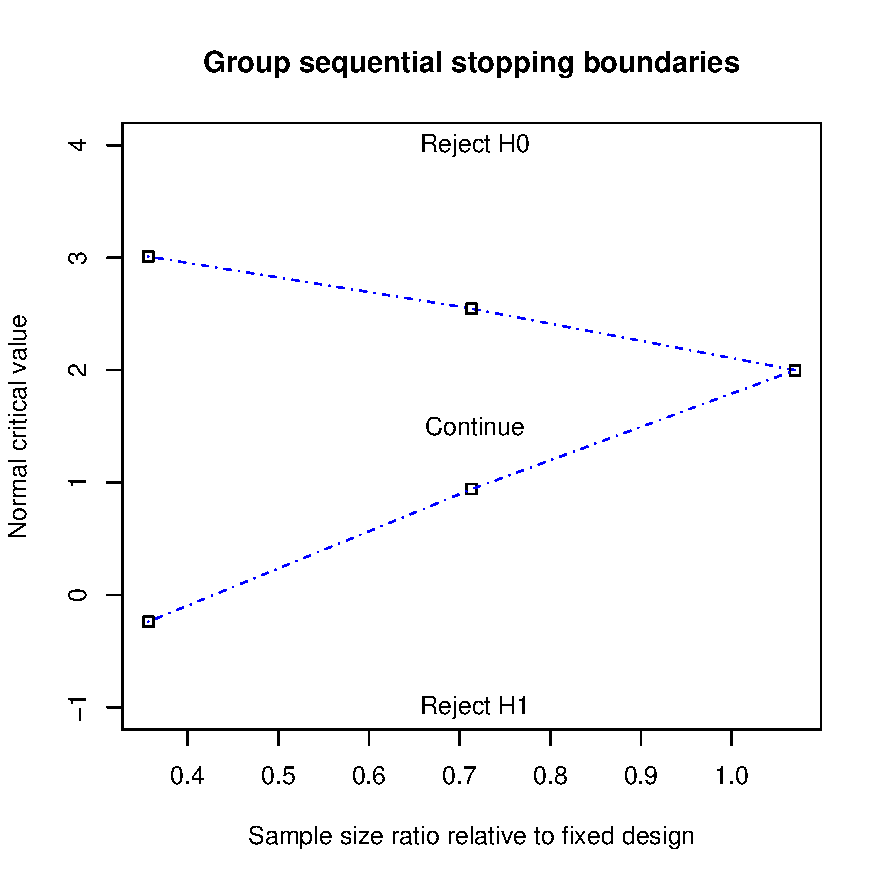
\includegraphics[width=.6\textwidth]{figs/boundplot.pdf}
\end{center}
\caption{Default plot for gsDesign object from example 1}
%RBC plot needs updating
\end{figure}%

\begin{figure}
\begin{center}
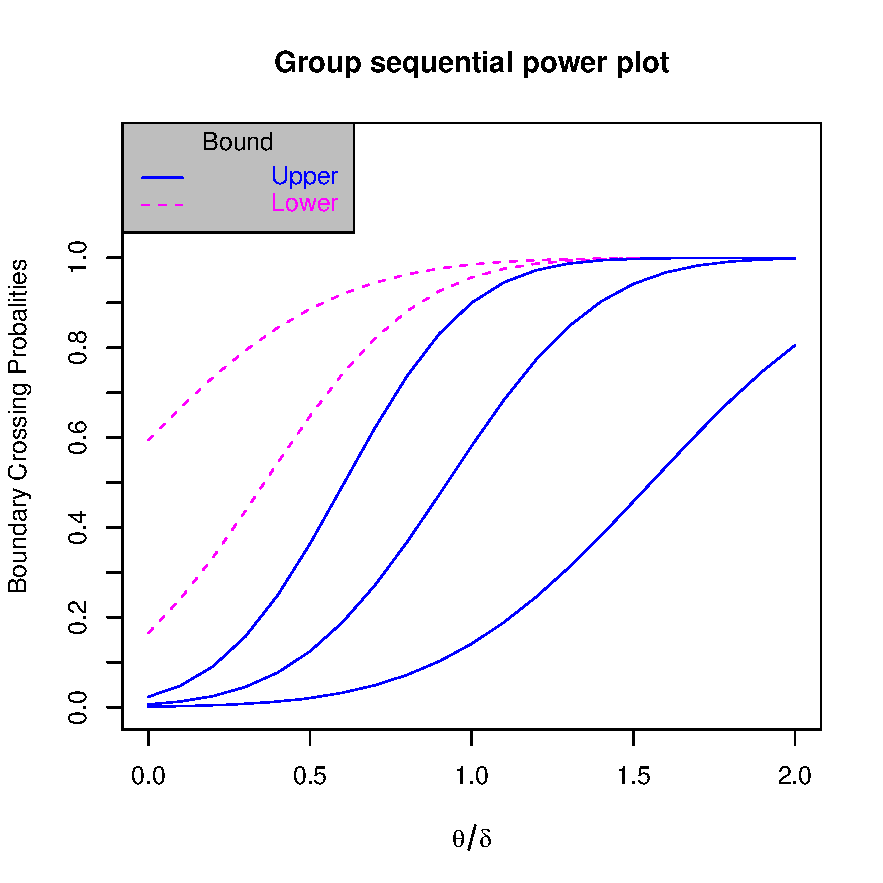
\includegraphics[width=.6\textwidth]{figs/powerplot.pdf}
\end{center}
\caption{Power plot (plottype=2) for gsDesign object from example 1}
\end{figure}%


\bigskip

Above we have seen standard output for \texttt{gsDesign()}. Now we look at how
to access individual items of information about what is returned from
\texttt{gsDesign()}. First, we use \texttt{summary(x)} to list the elements of
\texttt{x}. To view an individual element of \texttt{x}, we provide the
example \texttt{x\$delta}. See Section~\ref{sec:statmethods}, Statistical Methods, for an explanation of this value of \texttt{x\$delta}. Other elements of 
\texttt{x} can be accessed in the same way. Of particular interest are the 
elements \texttt{upper} and \texttt{lower}. These are both objects containing 
multiple variables concerning the upper and lower boundaries and boundary 
crossing probabilities.
The command summary \texttt{x\$upper} shows what these variables are. 
The upper boundary is shown with the command \texttt{x\$upper\$bound}.

\bigskip

\begin{verbatim}
> summary(x)
           Length Class   Mode     
k          1      -none-  numeric  
test.type  1      -none-  numeric  
alpha      1      -none-  numeric  
beta       1      -none-  numeric  
astar      1      -none-  numeric  
delta      1      -none-  numeric  
n.fix      1      -none-  numeric  
timing     3      -none-  numeric  
tol        1      -none-  numeric  
r          1      -none-  numeric  
n.I        3      -none-  numeric  
maxn.IPlan 1      -none-  numeric  
errcode    1      -none-  numeric  
errmsg     1      -none-  character
upper      9      spendfn list     
lower      9      spendfn list     
theta      2      -none-  numeric  
falseposnb 3      -none-  numeric  
en         2      -none-  numeric  
> x$delta
[1] 3.241516
> summary(x$upper)
        Length Class  Mode     
name    1      -none- character
param   1      -none- numeric  
parname 1      -none- character
sf      1      -none- function 
spend   3      -none- numeric  
bound   3      -none- numeric  
prob    6      -none- numeric  
errcode 1      -none- numeric  
errmsg  1      -none- character
> x$upper$bound
[1] 3.010739 2.546531 1.999226
\end{verbatim}

\bigskip
Now suppose you wish to design a trial for a binomial outcome to detect a
reduction in the primary endpoint from a 15\% event rate in the control group
to a 10\% rate in the experimental group. A trial with no interim analysis has
a sample size of 918 per arm or 1836 using \texttt{FarrMannSS()}. To get a
sample size for the above design, we compute interim and final sample sizes
(both arms combined) as follows:

\bigskip
\begin{verbatim}
> n.fix <- FarrMannSS(p1=.15, p2=.1, beta=.1, outtype=1)}
> n.fix
{[1] 1834.641
\end{verbatim}

\bigskip
%RBC--the following is a non-sequitur, based on the current text above. 
%RBC--originally, there was a call to ceiling(2*957*x$n.I), so one
%RBC--could see where the x$n.I reference came from. Now it just appears
%RBC--out of place. In particular, the value of 957 (which was attributed
%RBC--to nQuery) seems just wrong given the 918 above.
%RBC--see END NON-SEQUITUR comment below to see where things should be looked at
That is, we use \texttt{x\$n.I} to adjust a fixed sample size design and
obtain sample sizes for testing at the interim and final analyses. This method
of calculating \texttt{x\$n.I} is done automatically with the default input
value of \texttt{n.fix = 1}. The following gets this specific trial design with
the original call to \texttt{gsDesign()}, now with a calculated standardized
effect size of $\delta = 0.0741$:

\bigskip

\begin{verbatim}
> gsDesign(n.fix=2*957)
\end{verbatim}
\bigskip

If it were acceptable to use a logrank test for the above design with a fixed
follow-up period per patient, nQuery returns a sample size of 645 per arm for
a fixed design. In this case, the following sample sizes could be used at the
interim and final analyses (the ceiling function is used to round up):

\bigskip

\begin{verbatim}
> ceiling(gsDesign(n.fix=2*645)$n.I)
[1] 461 921 1381
\end{verbatim}
\bigskip

If, in addition, it were acceptable to assume the lower bound was binding, the
sample size would be:

\bigskip

\begin{verbatim}
> ceiling(gsDesign(n.fix=2*645,test.type=3)$n.I)
[1] 451 902 1353
\end{verbatim}
\bigskip
%RBC-- END NON SEQUITUR

Before we proceed to example 2, we consider some simple alternatives to the
standard spending function parameters. In the first code line following, we
replace lower and upper spending function parameters with $1$ and $-2$,
respectively; the default Hwang-Shih-DeCani spending function family is still
used. In the second line, we use a Kim-DeMets (power) spending function for
both lower and upper bounds with parameters $2$ and $3$, respectively. Then we
compare bounds with the above design.

\bigskip

\begin{verbatim}
> xHSDalt <- gsDesign(sflpar=1, sfupar=-2)
> xKD <- gsDesign(sfl=sfPower, sflpar=2, sfu=sfPower, sfupar=3)
> x$upper$bound
[1] 3.010739 2.546531 1.999226
> xHSDalt$upper$bound
[1] 2.677524 2.385418 2.063740
> xKD$upper$bound
[1] 3.113017 2.461933 2.008705
> x$lower$bound
[1] -0.2387240 0.9410673 1.9992264
> xHSDalt$lower$bound
[1] 0.3989132 1.3302944 2.0637399
> xKD$lower$bound
[1] -0.3497491 0.9822541 2.0087052
\end{verbatim}

\subsection*{Example 2: 2-sided testing, including pointwise spending,
O'Brien-Fleming, Pocock and Wang-Tsiatis designs}


For this example we consider a two-sided test with user-specified spending 
and five analyses with unequal spacing. We again assume the binomial example 
with fixed $n$ per arm of 957. Note the difference in labeling inside the 
plot due to the two-sided nature of testing. Note also that spending is 
printed as one-sided, and that only the upper spending function is needed/used. 
The cumulative spending at each analysis 
%RBC looks like something is missing here

\bigskip

\begin{verbatim}
> # Cumulative proportion of spending planned at each analysis
> p <- c(.05, .1, .15, .2, 1)
> # Cumulative spending intended at each analysis (for illustration)
> p * 0.025
[1] 0.00125 0.00250 0.00375 0.00500 0.02500
> # Incremental spending intended at each analysis
> # for comparison to spend column in output
> (p - c(0, p[0:4])) * 0.025
> x <- gsDesign(k=5, test.type=2, n.fix=1904, timing=c(.1,.25,.4,.6),
+ sfu=sfPoints,sfupar=p)
> x
Symmetric two-sided group sequential design with 90 % power and 2.5 % Type I Error.
Spending computations assume trial stops if a bound is crossed.

               
  Analysis   N   Z   Nominal p  Spend
         1  196 3.02    0.0013 0.0013
         2  488 2.99    0.0014 0.0013
         3  781 2.93    0.0017 0.0012
         4 1171 2.90    0.0019 0.0013
         5 1952 2.01    0.0222 0.0200
     Total                     0.0250 
++ alpha spending: User-specified spending function with Points = 0.05 0.1 0.15 0.2 1

Boundary crossing probabilities and expected sample size assuming any cross stops the trial

Upper boundary (power or Type I Error)
          Analysis
   Theta      1      2      3      4      5 Total   E{N}
  0.0000 0.0013 0.0013 0.0013 0.0013 0.0200 0.025 1938.4
  0.0743 0.0235 0.0758 0.1218 0.1760 0.5029 0.900 1519.1

Lower boundary (futility or Type II Error)
          Analysis
   Theta      1      2      3      4    5 Total
  0.0000 0.0013 0.0013 0.0013 0.0013 0.02 0.025
  0.0743 0.0000 0.0000 0.0000 0.0000 0.00 0.000
> plot(x)
\end{verbatim}

\begin{center}%
\begin{figure}
\begin{center}
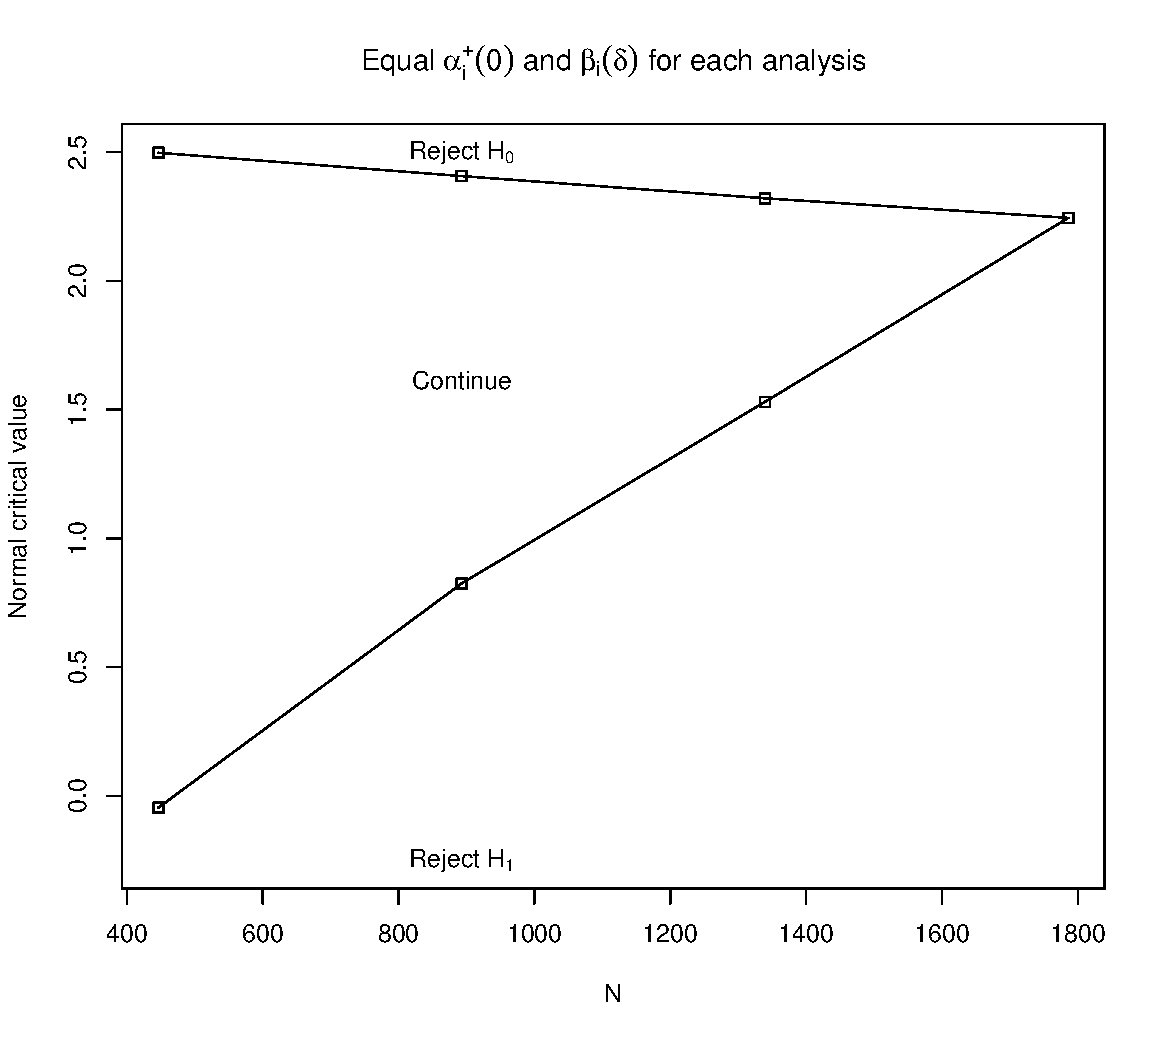
\includegraphics[width=.6\textwidth]{figs/boundplot2.pdf}
%RBC plot needs updating
\end{center}
\caption{Boundary plot for example 2}
\end{figure}%

\end{center}

O'Brien-Fleming, Pocock, or Wang-Tsiatis are normally used with equally-spaced
analyses. O'Brien-Fleming, Pocock, or Wang-Tsiatis (parameter of 0.4) bounds
for equally space analyses are generated as follows:

\bigskip

\begin{verbatim}
> xOF <- gsDesign(k=5, test.type=2, n.fix=1904, sfu="OF")
> xPk <- gsDesign(k=5, test.type=2, n.fix=1904, sfu="Pocock")
> xWT <- gsDesign(k=5, test.type=2, n.fix=1904, sfu="WT", sfupar=.4)
\end{verbatim}

\bigskip

Once you have generated these designs, examine the upper bounds as in 
Example~1.  Also, look at the spending by looking at, for example,
\texttt{xOF\$upper\$spend}.


\subsection*{Example 3: Logistic spending function}

Assume we would like the cumulative spending at 10\% of enrollment to be
$0.00125$ (5\% of total spending) and at 60\% of enrollment to be $0.005$ 
(20\% of total spending) so that $\alpha$-spending of $0.02$ is available for 
the final analysis; see \texttt{sfupar} in the following to find these 
numbers. This is the four-parameter specification of a logistic spending 
function (\texttt{sfLogistic()}, or the other two-parameter spending functions
\texttt{sfNormal()} and \texttt{sfCauchy()}). In each case, the four-parameter
specification is translated to the two essential parameters, but allows the
specification to be done simply.

\bigskip
\begin{verbatim}
> gsDesign(k=5, timing=c(.1, .25, .4, .6), test.type=2, n.fix=1904,
+ sfu=sfLogistic, sfupar=c(.1, .6, .05, .2))
Symmetric two-sided group sequential design with 90 % power and 2.5 % Type I Error.
Spending computations assume trial stops if a bound is crossed.

               
  Analysis   N   Z   Nominal p  Spend
         1  195 3.02    0.0013 0.0013
         2  488 3.04    0.0012 0.0011
         3  780 2.99    0.0014 0.0010
         4 1170 2.83    0.0023 0.0017
         5 1949 2.01    0.0223 0.0200
     Total                     0.0250 
++ alpha spending: Logistic spending function with a b = -1.629033 0.5986671

Boundary crossing probabilities and expected sample size assuming any cross stops the trial

Upper boundary (power or Type I Error)
          Analysis
   Theta      1      2      3      4     5 Total   E{N}
  0.0000 0.0013 0.0011 0.0010 0.0017 0.020 0.025 1936.1
  0.0743 0.0235 0.0686 0.1123 0.2077 0.488 0.900 1514.0

Lower boundary (futility or Type II Error)
          Analysis
   Theta      1      2     3      4    5 Total
  0.0000 0.0013 0.0011 0.001 0.0017 0.02 0.025
  0.0743 0.0000 0.0000 0.000 0.0000 0.00 0.000
\end{verbatim}
\bigskip

The same output can be obtained using the two-parameter specification of the
logistic spending function as follows (with values for \texttt{a} and 
\texttt{b} from above in \texttt{param}):

\bigskip

\begin{verbatim}
> y <- gsDesign(k=5, timing=c(.1, .25, .4, .6), test.type=2, n.fix=1904,
{+ sfu=sfogistic, sfupar=c(-1.629033, 0.5986671))
\end{verbatim}
\bigskip

To verify the initial spend is $0.00125$ (since it was rounded to 0.0013 above),
we examine the appropriate element of \texttt{y} just computed:

\bigskip

\begin{verbatim}
> y$upper$spend[1]
[1] 0.00125
\end{verbatim}


\subsection*{Example 4: gsProbability()}


We reconsider Example~1 and obtain the properties for the design for a larger
set of $\theta$ values than in the standard printout for \texttt{gsDesign()}.
The standard plot design for a \texttt{gsProbability} object is the power plot 
shown in Example~1. The boundary plot is obtainable below using the command
\texttt{plot(y, plottype=1)}.

\bigskip

\begin{verbatim}
> x <- gsDesign()
> y <- gsProbability(theta=x$delta*seq(0, 2, .25), d=x)
> y 
Asymmetric two-sided group sequential design with 90 % power and 2.5 % Type I Error.
Upper bound spending computations assume trial continues if lower bound is crossed.

           Sample
            Size    ----Lower bounds----  ----Upper bounds-----
  Analysis Ratio*   Z   Nominal p Spend+  Z   Nominal p Spend++
         1  0.357 -0.24    0.4057 0.0148 3.01    0.0013  0.0013
         2  0.713  0.94    0.8267 0.0289 2.55    0.0054  0.0049
         3  1.070  2.00    0.9772 0.0563 2.00    0.0228  0.0188
     Total                        0.1000                 0.0250 
+ lower bound beta spending (under H1): Hwang-Shih-DeCani spending function with gamma = -2
++ alpha spending: Hwang-Shih-DeCani spending function with gamma = -4
* Sample size ratio compared to fixed non-group sequential design

Boundary crossing probabilities and expected sample size assuming any cross stops the trial

Upper boundary (power or Type I Error)
          Analysis
   Theta      1      2      3  Total   E{N}
  0.0000 0.0013 0.0049 0.0171 0.0233 0.6249
  0.8104 0.0058 0.0279 0.0872 0.1209 0.7523
  1.6208 0.0205 0.1038 0.2393 0.3636 0.8520
  2.4311 0.0595 0.2579 0.3636 0.6810 0.8668
  3.2415 0.1412 0.4403 0.3185 0.9000 0.7913
  4.0519 0.2773 0.5353 0.1684 0.9810 0.6765
  4.8623 0.4574 0.4844 0.0559 0.9976 0.5701
  5.6727 0.6469 0.3410 0.0119 0.9998 0.4868
  6.4830 0.8053 0.1930 0.0016 1.0000 0.4266

Lower boundary (futility or Type II Error)
          Analysis
   Theta      1      2      3  Total
  0.0000 0.4057 0.4290 0.1420 0.9767
  0.8104 0.2349 0.3812 0.2630 0.8791
  1.6208 0.1138 0.2385 0.2841 0.6364
  2.4311 0.0455 0.1017 0.1718 0.3190
  3.2415 0.0148 0.0289 0.0563 0.1000
  4.0519 0.0039 0.0054 0.0097 0.0190
  4.8623 0.0008 0.0006 0.0009 0.0024
  5.6727 0.0001 0.0001 0.0000 0.0002
  6.4830 0.0000 0.0000 0.0000 0.0000
\end{verbatim}

\subsection*{Example 5: Non-inferiority testing }

We consider a trial examining a new drug that is more convenient to administer
than an approved control. There is no expectation of a substantially improved
response with the new drug. While the new drug may be a little better or
worse than control, there is some suggestion that the new drug may not be as
efficacious as control. Rather than powering the trial to show non-inferiority
when the new drug is slightly worse than control, the strategy is taken to
stop the trial early for futility if there is a `substantial' trend towards
the new drug being inferior. The control drug has provided a (binomial)
response rate of 67.7\% in a past trial and regulators have agreed with a
non-inferiority margin of 7\%. Let the underlying event rate in the control
and experimental groups be denoted by $p_{C}$ and $p_{E}$, respectively. Let
$\delta = 0.07$ represent the non-inferiority margin. There is no desire to stop
the trial early to establish non-inferiority. That is, this is a one-sided
testing problem for interim analyses. We let H$_{0}$: $p_{C}-p_{A}\leq0$ and
test against the alternative H$_{1}$: $p_{C}-p_{A}\geq\delta$., only stopping
early if H$_{0}$ can be rejected.\ We must have 97.5\% power to reject H$_{0}$
when H$_{1}$ is true ($\beta=0.025$) and can have a 10\% chance of rejecting
H$_{0}$ when H$_{0}$ is true ($\alpha=0.1$). In this case, an aggressive
stopping boundary is desirable to stop the trial 40\% of the way through
enrollment if the experimental drug is, in fact, not as efficacious as
control. The routine \texttt{FarrMannSS()} included with this package uses the
method of Farrington and Manning \cite{FarringtonManning}\ to compute the sample
size for a two-arm binomial trial for superiority or non-inferiority; see the
help file for documentation. As shown below, this requires 1966 patients for a
trial with no interim analysis; both nQuery and PASS2005 also yield this
result. Using this fixed sample size as input to \texttt{gsDesign()} yields a
sample size of 2332 for the trial compared to 2333 from EAST\ 5.2. This design
requires less than approximately a 4.5\% difference in event rates at the
interim analysis to continue and a final difference of no more than
approximately 3.3\% to achieve non-inferiority. These differences were
carefully evaluated in choosing the appropriate value of \texttt{gamma} for
the spending function.

\bigskip

\begin{verbatim}
> n.fix <- FarrMannSS(p1=.607, p2=.677, alpha=.1, beta=.025, sided=1, outtype=1)
> n.fix
[1] 1965.059
> gsDesign(k=2, alpha=.1, beta=.025, n.fix=n.fix, test.type=1, sfupar=3, timing=.4)
One-sided group sequential design with 97.5 % power and 10 % Type I Error.
               
  Analysis   N   Z   Nominal p  Spend
         1  933 1.45    0.0735 0.0735
         2 2332 1.68    0.0468 0.0265
     Total                     0.1000 
++ alpha spending: Hwang-Shih-DeCani spending function with gamma = 3

Boundary crossing probabilities and expected sample size assuming any cross stops the trial

Upper boundary (power or Type I Error)
          Analysis
   Theta      1      2 Total   E{N}
  0.0000 0.0735 0.0265 0.100 2228.7
  0.0731 0.7832 0.1918 0.975 1235.8
\end{verbatim}

\subsection*{Example 6: Non-inferiority and superiority testing in the same trial }


We consider a safety trial where a drug is given chronically to patients who
are expected to have a 3.5\% annual risk (exponential parameter $\lambda
_{0}=-\ln(1-0.035)=0.035627$) of developing cardiovascular disease (CVD) and
we wish to rule out an elevated risk that would be indicated by a hazard ratio
of 1.2 ($\lambda_{1}=1.2\lambda_{0}=0.042753)$. The desire is that if there is
a hazard ratio of 1.2 that there is at most a 2.5\% chance of demonstrating
non-inferiority. On the other hand, if the true hazard ratio is 1 (no excess
risk), we wish to have a 90\% probability of showing `no disadvantage'
(that is, we wish to rule out $\lambda_{1}\geq1.2\lambda_{0}$). In
hypothesis testing terms, the role of the null hypothesis (no difference) and
alternative hypothesis (20\% increased hazard ratio) have been reversed. We
label the hypotheses as before, but the error levels are reversed to
satisfy the above. We let the null hypothesis of no difference be denoted by
H$_{0}$: $\log(\lambda_{1}/\lambda_{0})=0$ and the alternate hypothesis is denoted by H$_{1}$: $\log(\lambda_{1}/\lambda_{0})=\log(1.2).$ To achieve
the desired performance, Type I error is set to 10\% and Type II error is set
to 2.5\%. Assume the trial is to be enrolled in a 2-year period and the
dropout rate is 15\% per year ($\lambda_{D}=-\ln(1-0.15)=0.162519$). As seen
below, fixed design with no interim analysis requires a sample size of 6,386
per treatment group to obtain 1,570 total events (under in 6 years H$_{1}$).
Note that under the null hypothesis, the overall event rate would be lower and
it would take longer to obtain the number of events required.

\bigskip
\begin{verbatim}
> # exponential control group failure rate of 3.5 percent per year
> lambda.0 <- -log(1-.035)
> # wish to rule out experimental group hazard ratio of 1.2 
> lambda.1 <- 1.2*lambda.0
> # dropout rate of 15 percent per year
> eta <-  -log(1-.15)
> # fixed design sample size
> # recruitment time Tr=2 years, total study time Ts=6 years
> SSFix <-nSurvival(lambda.0=lambda.0, lambda.1=lambda.1, eta=eta, alpha=.1, beta=.025,
+ type="rr", Ts=6, Tr=2)
> # show sample size per group and total number of events required for fixed design
> ceiling(SSFix$Sample.size/2)
[1] 6386
> ceiling(SSFix$Num.events)
[1] 1570
\end{verbatim}
\bigskip

We use the above sample size and number of events below to adjust this
fixed design to a group sequential design and obtain the number of events
required at each analysis. In addition, we consider the possibility that the
experimental drug may actually reduce cardiovascular risk. For a fixed design,
superiority testing may be performed following non-inferiority testing. For a
group sequential trial, the situation is slightly more complex; this is not a
scenario that can be dealt with in EAST 5.2. We take two approaches to this.
First, we consider non-inferiority of control to treatment to be of no
interest, which leads to an asymmetric design. Second, we consider the problem
to be symmetric: inference on one arm relative to the other uses identical
criteria; this will be deferred to example 7
%RBC: there is currently no example 7

Let H$_{0}$: $\theta = 0$ and H$_{1}$: $\theta\neq0$ where $\theta$ indicates
the underlying difference between two treatment groups. We wish to show that a
new treatment is non-inferior compared to control. That is, for some
$\delta > 0,$ under H$_{1A}$: $\theta = \delta$ we wish to have 97.5\% power to
reject H$_{0}$: $\theta = 0$ (i.e., \texttt{beta=0.025} to yield a 2.5\% chance
of accepting non-inferiority when in fact the underlying effect for the
experimental group is higher by $\delta$). On the other hand, under H$_{0}$:
$\theta=0$ we are willing to have a 10\% chance of rejecting H$_{0} $:
$\theta=0$ in favor of H$_{1A}$: $\theta=\delta$ (\texttt{alpha=0.10} to yield
90\% power to show non-inferiority). We have a slightly asymmetric test for
superiority in that we would like to reject H$_{0}$: $\theta$=0 in favor of
H$_{1B}$: $\theta=-\delta$ at the 2.5\% (one-sided) level 
(\texttt{astar=0.025}) to control Type I error in that direction. Thus, 
the trial could stop early if $\theta$ is substantially different from $0$ 
in either direction. A Hwang-Shih-DeCani spending function with 
\texttt{sfupar=sflpar=-4} is used for
each bound. The bounds are asymmetric due to the different levels of the test
in each direction. The appropriate confidence interval approach for this
design is probably a stage-wise ordering approach (see Jennison \& Turnbull
\cite{JTBook}, sections 8.4 and 8.5). This gives the tightest intervals at
the end of the trial and does not result in conflicts between the confidence
intervals and the testing approach just outlined.

See output below for a design with four equally spaced interims. With
\texttt{n.fix=1264} we find that $\delta=0.0818$. Interestingly, there is
90\% power to cross the lower bound under H$_{1B}$: $\theta = -\delta$, so the
trial is well-powered for superiority of the experimental treatment. The
design requires an increase from 1570 events to 1595 in order to maintain the
desired error rates with the given stopping rules. Note that
\texttt{test.type=5} indicates that all bounds are binding and both upper and
lower bound error spending is under the null hypothesis. The upper bound is a
futility bound for showing non-inferiority. If it is never crossed, the trial
establishes non-inferiority. The lower bound is the superiority bound.

\bigskip
\begin{verbatim}
> # show number of events required at interim and final analysis
> # of group sequential design
> x <- gsDesign(test.type=5, k=5, alpha=.1, beta=.025, astar=.025, sflpar=-4,
+               sfupar=-4, n.fix=SSFix$Num.events)
>
> # show sample size per group required using same inflation factor as
> # for number of events
> ceiling(x$n.I[5]/SSFix$Num.events*SSFix$Sample.size/2)}
[1] 6491
>
> # show power at + or - delta and 0
> y <- gsProbability(d=x, theta=c(-x$delta, 0, x$delta))
> y
Asymmetric two-sided group sequential design with 97.5 % power and 10 % Type I Error.
Spending computations assume trial stops if a bound is crossed.

                  ----Lower bounds----  ----Upper bounds-----
  Analysis   N    Z   Nominal p Spend+  Z   Nominal p Spend++
         1  319 -3.25    0.0006 0.0006 2.84    0.0023  0.0023
         2  638 -2.99    0.0014 0.0013 2.52    0.0059  0.0051
         3  957 -2.69    0.0036 0.0028 2.17    0.0150  0.0113
         4 1276 -2.37    0.0088 0.0063 1.78    0.0376  0.0252
         5 1595 -2.03    0.0214 0.0140 1.33    0.0916  0.0561
     Total                      0.0250                 0.1000 
+ lower bound spending (under H0): Hwang-Shih-DeCani spending function with gamma = -4
++ alpha spending: Hwang-Shih-DeCani spending function with gamma = -4

Boundary crossing probabilities and expected sample size assuming any cross stops the trial

Upper boundary (power or Type I Error)
          Analysis
    Theta      1      2      3      4      5 Total   E{N}
  -0.0818 0.0000 0.0000 0.0000 0.0000 0.0000 0.000 1150.8
   0.0000 0.0023 0.0051 0.0113 0.0252 0.0561 0.100 1566.1
   0.0818 0.0847 0.2516 0.3181 0.2255 0.0951 0.975  971.2

Lower boundary (futility or Type II Error)
          Analysis
    Theta      1      2      3      4      5 Total
  -0.0818 0.0366 0.1497 0.2632 0.2700 0.1785 0.898
   0.0000 0.0006 0.0013 0.0028 0.0063 0.0140 0.025
   0.0818 0.0000 0.0000 0.0000 0.0000 0.0000 0.000
> plot(y, plottype="xbar")
\end{verbatim}
\bigskip

The plot below shows the cumulative probabilities of stopping at each analysis
for different values of $\theta$. The solid lines go from the probability of
stopping at the first interim analysis to the highest line which shows the
probability of an inferiority finding at any analysis. The dashed lines
provide 1 minus the cumulative probability of stopping for superiority for
different values of $\theta$ for each analysis. Note that the expected sample
size required to come to a conclusion if the experimental regiment is truly
inferior to control (H$_{1A}$: $\theta = \delta$) is 653 events compared to 1264
for a fixed design. In addition, there is only a 6.8\% chance of continuing
the trial to the final analysis. This is comprised of a 2.5\% of continuing
the trial to the final analysis and falsely establishing non-inferiority plus a
4.27\% of continuing to the trial to the final analysis to establish
inferiority. If experimental therapy is truly superior, the expected number of
events required to demonstrate a difference is 950. If there is truly no
difference the trial usually goes to the end (about 91\% of the time; this is
seen by the last result below) and finds no difference (87.5\% of the time;
this is the sum of the Type I error in both directions).

Evaluation of the cutoffs has not been performed as in Example 5. This
exercise would be worthwhile to verify that the cutoffs of the design are appropriate.

\bigskip
\begin{verbatim}
> x <- gsDesign(test.type=5, k=5, alpha=.1, beta=.025, astar=.025, sflpar=-3,
+ sfupar=0, n.fix=1264)
> y <- gsProbability(d=x, theta=c(-x$delta, 0, x$delta))
> y
Asymmetric two-sided group sequential design with 97.5 % power and 10 % Type I Error.
Spending computations assume trial stops if a bound is crossed.

                  ----Lower bounds----  ----Upper bounds-----
  Analysis   N    Z   Nominal p Spend+  Z   Nominal p Spend++
         1  284 -3.07    0.0011 0.0011 2.05    0.0200    0.02
         2  567 -2.84    0.0022 0.0020 1.91    0.0278    0.02
         3  850 -2.60    0.0047 0.0036 1.79    0.0368    0.02
         4 1133 -2.34    0.0097 0.0065 1.68    0.0465    0.02
         5 1417 -2.06    0.0197 0.0119 1.58    0.0568    0.02
     Total                      0.0250                 0.1000 
+ lower bound spending (under H0): Hwang-Shih-DeCani spending function with gamma = -3
++ alpha spending: Hwang-Shih-DeCani spending function with gamma = 0

Boundary crossing probabilities and expected sample size assuming any cross stops the trial

Upper boundary (power or Type I Error)
          Analysis
    Theta      1     2      3      4      5  Total   E{N}
  -0.0912 0.0002 0.000 0.0000 0.0000 0.0000 0.0002  950.0
   0.0000 0.0200 0.020 0.0200 0.0200 0.0200 0.1000 1352.8
   0.0912 0.3018 0.325 0.2048 0.1007 0.0427 0.9750  653.6

Lower boundary (futility or Type II Error)
          Analysis
    Theta      1      2      3      4      5  Total
  -0.0912 0.0625 0.1988 0.2796 0.2396 0.1401 0.9207
   0.0000 0.0011 0.0020 0.0036 0.0065 0.0119 0.0250
   0.0912 0.0000 0.0000 0.0000 0.0000 0.0000 0.0000
> plot(gsProbability(k=5, n.I=x$n.I, a=x$lower$bound, b=x$upper$bound,
+ theta=x$delta*(-25:25)/25))
> # compute probability of continuing to the end of the trial under H0
> 1-sum(y$upper$prob[1:4, 2] + y$lower$prob[1:4, 2])
[1] 0.9068707
\end{verbatim}

\begin{center}%
\begin{figure}
\begin{center}
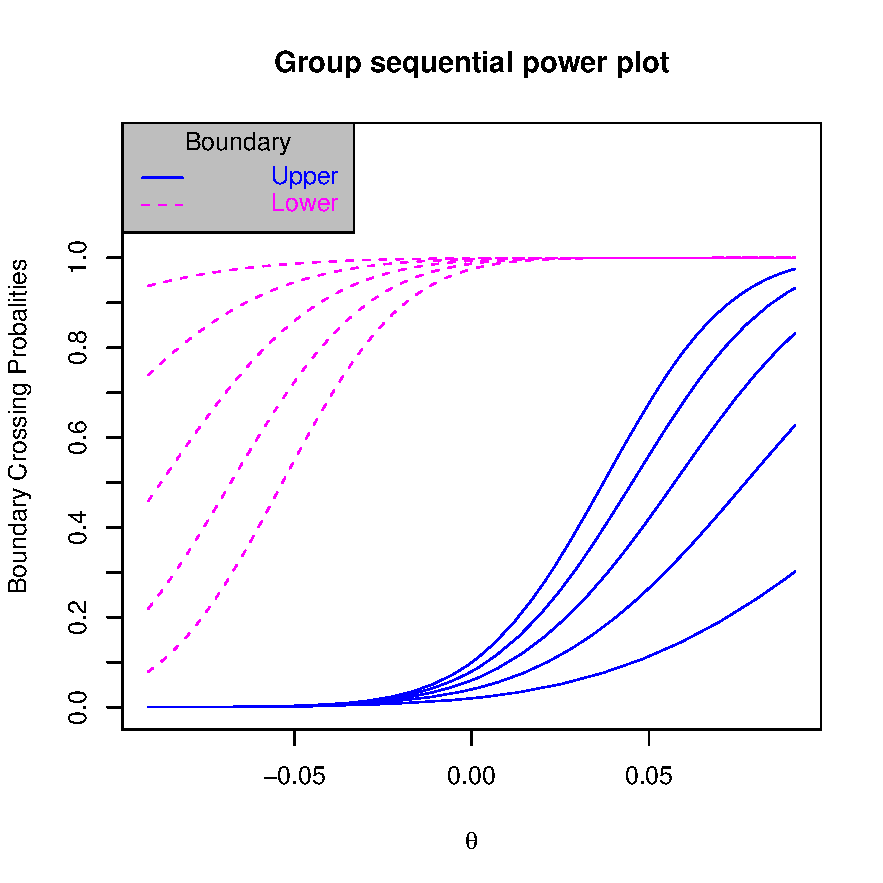
\includegraphics[width=.6\textwidth]{figs/noninferiority.pdf}
\end{center}
\caption{Power plot for non-inferiority design in example 6}
\end{figure}%

\end{center}


\section{Syntax}

The two primary functions available in this package are:

\begin{itemize}
\item \texttt{gsDesign(argument1 = value1, \ldots)}

\item \texttt{gsProbability(argument1 = value1, \ldots)}
\end{itemize}

All arguments are in lower case with the exception of \texttt{n.I} in
\texttt{gsProbability()}. Although there are many arguments available in
\texttt{gsDesign()}, many of these need not be specified as the defaults are adequate. Returned values from \texttt{gsDesign()} and
\texttt{gsProbability()} are objects from newly defined classes named 
\texttt{gsDesign} and \texttt{gsProbability}. The \texttt{gsDesign} class is 
an extension of (inherits the characteristics of) the \texttt{gsProbability} 
class. These classes are described in
Section~\ref{sec:objtypes}, The \texttt{gsDesign} and \texttt{gsProbability} 
Object Types. The output functions \texttt{print()}, and \texttt{plot()} 
for the \texttt{gsDesign} and \texttt{gsProbability} classes are described 
further in Section~\ref{sec:formatted}, Formatted Output.

In the following, there is a single parameter $\theta$ for which we generally
are trying to test a null hypothesis H$_{0}$: $\theta=0$ against some
alternative such as H1: $\theta$ $\neq0$. In general, the parameter $\theta$
is a standardized treatment difference and the statistic $Z_{n}$
for testing after $n$ observations have a distribution that is well
approximated by a normal distribution with mean $\sqrt{n}\theta$ and variance
1. See Jennison and Turnbull \cite{JTBook} for extensive discussions of
various types of endpoints for which the approximation is reasonable. For
example, normal, binomial and time-to-event endpoints may be considered.
Section~\ref{sec:statmethods}, Statistical Methods, provides more detail.

As a supplement to the primary functions \texttt{gsDesign()} and
\texttt{gsProbability()}, we also consider functions \texttt{gsCP()} and
\texttt{gsBoundCP()}\ which compute the conditional probabilities of boundary
crossing. Background for conditional power computations is also provided in 
Section~\ref{sec:statmethods}, Statistical Methods.

Finally, some utility functions for working with two-arm binomial or survival
trials are provided. For the binomial distribution there are functions for
fixed (non-group-sequential) designs that compute sample size, perform
statistical testing, and perform simulations. For survival, a sample size
function is provided.

\subsection{gsDesign() syntax}

As noted above, \texttt{gsDesign()} provides sample size and boundaries for a
group sequential design based on treatment effect, spending functions for
boundary crossing probabilities, and relative timing of each analysis. The
most general form of the call to \texttt{gsDesign()} with default arguments is:

\bigskip

\texttt{gsDesign(k=3, test.type=4, alpha=0.025, beta=0.1, astar=0, delta=0,
n.fix=1,}

\texttt{\ \ \ timing=1, sfu=sfHSD, sfupar= -4, sfl=sfHSD, sflpar= -2,
tol=0.000001, r=18}

\texttt{\ \ \ n.I=0,maxn.IPlan=0)}.

\bigskip

The arguments are as follows:

\begin{itemize}
\item \texttt{k} = integer (\texttt{k}%
%TCIMACRO{\TEXTsymbol{>}}%
%BeginExpansion
$>$%
%EndExpansion
1). Specifies the number of analyses, including interim and final. The default
value is 3. {\bf Note:} Use of very large \texttt{k} produces an error
message. How large varies with the value of \texttt{test.type} specified. For
example, with default arguments (\texttt{test.type=3}), specifying \texttt{k}
%TCIMACRO{\TEXTsymbol{>} }%
%BeginExpansion
$>$
%EndExpansion
23 produces the error message "False negative rates not achieved." For
other values of \texttt{test.type}, the upper limit is larger.

\item \texttt{test.type} = integer (1$\leq$ \texttt{test.type} $\leq$ 6). In
the following we denote by $\theta$ the parameter we are testing for. The
null hypothesis will always be H$_{0}$: $\theta=0$. The alternative hypothesis
of interest varies with the value of \texttt{test.type}.

\begin{description}
\item[=1:] One-sided testing. Tests the null hypothesis H$_{0}$: $\theta=0$
against the alternative hypothesis H$_{1}$: $\theta>0$. The user specifies only
upper boundary crossing probabilities under the null hypothesis. There is no
lower boundary.

\item[=2:] Symmetric, two-sided testing. Tests H$_{0}$: $\theta = 0$ against the
alternative hypothesis H1: $\theta \neq 0$. Boundary crossing probabilities
are specified under the null hypothesis. The user specifies only upper boundary
crossing probabilities

\item[=3:] Asymmetric two-sided testing with binding lower bound and beta
spending. Asymmetric two-sided testing is also often referred to as two
one-sided tests in that testing is done both for efficacy (attempts to reject
H$_{0}$: $\theta = 0$ in favor of H$_{1}$: $\theta > 0$) and futility 
(attempts to reject H$_{1}$: $\theta$ = \texttt{delta} in favor of H$_{0}$: $\theta$
%TCIMACRO{\TEXTsymbol{<} }%
%BeginExpansion
$<$
%EndExpansion
\texttt{delta}). Upper and lower boundary crossing probabilities are
asymmetric. Upper boundary crossing probabilities are specified under H$_{0}$:
$\theta=0$ ($\alpha-$spending). Lower boundary crossing probabilities are
specified under H$_{1}$: $\theta$ = \texttt{delta} ($\beta-$spending).
Computation of upper boundary crossing probabilities under the null hypothesis
(Type I error) assumes the lower boundary is binding; that is, the trial 
{\em must} stop if the lower boundary is crossed. See Section~\ref{sec:statmethods}, Statistical Methods, for details on
boundary crossing probabilities for options 3 through 6.

\item[=4:] Default. Asymmetric two-sided testing with non-binding lower bound
and beta spending. Same as \texttt{test.type=3}, except that Type I error
computation assumes lower boundary is non-binding; that is, the calculation
assumes that the trial stops only if the upper boundary is crossed---it will
continue if the lower boundary is crossed. Type II error computation assumes
the trial will stop when either boundary is crossed. The effect of this is to
raise the upper boundaries after the first interim analysis relative to
\texttt{test.type=3}. See Section~\ref{sec:statmethods}, Statistical Methods, for details.

\item[=5:] Asymmetric two-sided testing with binding lower bound and lower bound
spending specified under the null hypothesis. Same as \texttt{test.type=3},
except that lower boundary crossing probabilities are specified under H$_{0}$:
$\theta=0$. See Section~\ref{sec:statmethods}, Statistical Methods, for details.

\item[=6:] Asymmetric two-sided testing with non-binding lower bound and lower
bound spending specified under the null hypothesis. Same as 
\texttt{test.type=4}, except that lower boundary crossing probabilities are 
specified under H$_{0}$: $\theta=0$. See Section~\ref{sec:statmethods}, 
Statistical Methods, for details.
\end{description}

\item \texttt{alpha} = probability value (real; 0
%TCIMACRO{\TEXTsymbol{<} }%
%BeginExpansion
$<$
%EndExpansion
\texttt{alpha}
%TCIMACRO{\TEXTsymbol{<} }%
%BeginExpansion
$<$
%EndExpansion
1; for \texttt{test.type=2}, must have \texttt{alpha}
%TCIMACRO{\TEXTsymbol{<} }%
%BeginExpansion
$<$
%EndExpansion
0.5). Specifies the total Type I error summed across all analyses. For all
design types (including symmetric, two-sided) this is the probability of
crossing the upper boundary under the null hypothesis. The default value is
$0.025$. For symmetric, two-sided testing (\texttt{test.type=2}), this 
translates into 0.05 for the combined total probability of crossing a 
lower or upper bound at any analysis. See 
Section~\ref{sec:statmethods}, Statistical Methods, for details.

\item \texttt{beta} = probability value (real; 0
%TCIMACRO{\TEXTsymbol{<} }%
%BeginExpansion
$<$
%EndExpansion
\texttt{beta}
%TCIMACRO{\TEXTsymbol{<} }%
%BeginExpansion
$<$
%EndExpansion
1 - \texttt{alpha}). Specifies the total Type II error summed across all
analyses. The default value is $0.1$, which corresponds to 90\% power.

\item \texttt{astar} = probability value (real; 0 $\leq$ \texttt{astar} 
$\leq 1 -$ \texttt{alpha}). Normally not specified. If \texttt{test.type=5} or 
\texttt{test.type=6},
\texttt{astar} specifies the probability of crossing a lower bound at all
analyses combined. This is changed to $1 - $\texttt{alpha} when the default 
value of 0 is used. Since this is the expected usage, \texttt{astar} is 
not normally specified by the user.

\item \texttt{delta} = real value ($\delta > 0$). This is the standardized
effect size used for alternative hypothesis for which the design is powered.
If \texttt{delta}
%TCIMACRO{\TEXTsymbol{>} }%
%BeginExpansion
$>$
%EndExpansion
0, sample size is determined using this effect size (see 
Section~\ref{sec:statmethods}, Statistical Methods, for details); If the 
default \texttt{delta = 0} is given, sample size is
determined by \texttt{n.fix} as noted below. Only one of \texttt{delta} and
\texttt{n.fix} need be specified by the user.

\item \texttt{n.fix} = real value (\texttt{n.fix}
%TCIMACRO{\TEXTsymbol{>} }%
%BeginExpansion
$>$
%EndExpansion
0). If \texttt{delta}%
%TCIMACRO{\TEXTsymbol{>}}%
%BeginExpansion
$>$%
%EndExpansion
0 then \texttt{n.fix} is ignored. For the default values (\texttt{delta = 0} and
\texttt{n.fix = 1}) the returned values (R$_{1}$, \ldots, R$_{K}$) for sample
sizes are actually sample size ratios compared to a fixed design with no
interim analysis, where the denominator for all of these ratios is the sample
size for a fixed design with no interim analysis based on input values of
\texttt{alpha} and \texttt{beta}. If \texttt{delta = 0} and \texttt{n.fix}
%TCIMACRO{\TEXTsymbol{>} }%
%BeginExpansion
$>$
%EndExpansion
1, think of \texttt{n.fix} as the fixed sample size of a study without interim
analysis for the given values of \texttt{alpha} and \texttt{beta}.
\texttt{gsDesign()} then inflates this value to get a maximum sample size
to give the specified Type II error/power for the specified group sequential
design. We also denote \texttt{n.fix} as $N_{fix}$ below. See 
Section~\ref{sec:statmethods}, Statistical Methods,
for details on how to calculate sample size.

\item \texttt{timing} = 1 or \texttt{c(t}$_{\mathtt{1}}$\texttt{, \ldots,
t}$_{\mathtt{k-1}}$\texttt{)} or \texttt{c(t}$_{\mathtt{1}}$\texttt{, \ldots, 
t}$_{\mathtt{k}}$\texttt{)} where 0 %
%TCIMACRO{\TEXTsymbol{<}}%
%BeginExpansion
$<$%
%EndExpansion
 \texttt{t}$_{\mathtt{1}}$ 
%TCIMACRO{\TEXTsymbol{<}}%
%BeginExpansion
$<$%
%EndExpansion
 \ldots %
%TCIMACRO{\TEXTsymbol{<}}%
%BeginExpansion
$<$%
%EndExpansion
 \texttt{t}$_{k}$ = 1. Specifies the cumulative proportionate timing for
analyses; for example, \texttt{t}$_{\mathtt{2}} = 0.4$ means the second interim 
includes the first 40\% of planned observations. For equal spacing,
\texttt{timing = 1} (default), the timing is determined by the number of
interim looks \texttt{k}.

\item \texttt{sfu} = spending function (default = \texttt{sfHSD}). The
parameter sfu specifies the upper boundary using a spending function. For
one-sided and symmetric two-sided testing (\texttt{test.type}=1, 2),
\texttt{sfu} is the only spending function required to specify spending. The
default value is \texttt{sfHSD}, which is a Hwang-Shih-DeCani spending
function. See Section~\ref{sec:spendfun}, Spending Functions, for details on
the available options.

\item \texttt{sfupar} = real value (default = $-4$) The parameter
\texttt{sfupar} specifies any parameters needed for the spending function
specified by \texttt{sfu}. The default of $-4$ when used with the default
\texttt{sfu=sfHSD} provides a conservative, O'Brien-Fleming-like upper bound.
For spending functions that do not require parameters this is ignored.
Again, see Section~\ref{sec:spendfun}, Spending Functions, for details.

\item \texttt{sfl} = spending function (default = \texttt{sfHSD}). Specifies
the spending function for lower boundary crossing probabilities. The parameter
\texttt{sfl} is ignored for one-sided testing (\texttt{test.type = 1}) or
symmetric two-sided testing (\texttt{test.type = 2}).

\item \texttt{sflpar} = real value (default = $-2$). The parameter
\texttt{sflpar} specifies any parameters needed for the spending function
specified by \texttt{sfl}. The default value of $-2$ when used with the default
\texttt{sfl=sfHSD} provides a somewhat conservative lower bound. For spending
functions that do not require parameters this is ignored.

\item \texttt{tol} = value. Specifies the stopping increment for iterative
root-finding algorithms used to derive the user-specified design. The default
value is $0.000001$; must be
%TCIMACRO{\TEXTsymbol{>}}%
%BeginExpansion
$>$%
%EndExpansion
0 and $\leq 0.1$. This should probably be ignored by the user, but is provided
as a tuning parameter.

\item \texttt{r} = positive integer up to 80 (default = 18). This is a
parameter used to set the grid size for numerical integration computations;
see Jennison and Turnbull \cite{JTBook}, Chapter 19. This should probably be
ignored by the user, but is provided as a tuning parameter.

\item \texttt{n.I} = 
%RBC equals what?
Used for re-setting bounds when timing of analyses changes
from initial design; see Section~\ref{sec:reset}, Resetting Timing of Analyses.

\item \texttt{maxn.I} = 
%RBC equals what? "maxn.I=PlanUsed" was original text...
Used for re-setting bounds when timing of analyses
changes from initial design; see Section~\ref{sec:reset}, Resetting Timing of Analyses.
\end{itemize}

\subsection{gsProbability() syntax}

\texttt{gsProbability()} computes boundary crossing probabilities and expected
sample size of a design for arbitrary user-specified treatment effects,
interim analysis times, and bounds. The value returned has class
\texttt{gsProbability} as described in 
Section~\ref{sec:objtypes}, The \texttt{gsDesign} and \texttt{gsProbability} 
Object Types. The generic call to \texttt{gsProbability()} is of the form:

\bigskip

\texttt{gsProbability(k = 0, theta, n.I, a, b, r = 18, d=NULL)}

\bigskip

The value of \texttt{theta} must always be specified. This function is
designed to be called in one of two ways. First, using a returned value from a
call to \texttt{gsDesign()} in the input parameter \texttt{d}. If \texttt{d}
is non-null, the parameterization specified there determines the output rather
than the values of \texttt{k}, \texttt{n.I}, \texttt{a}, \texttt{b}, and
\texttt{r}. If \texttt{k} is not the default of 0, the user must specify the
set of input variables \texttt{k}, \texttt{n.I}, \texttt{a}, \texttt{b}, and
\texttt{r}. In the latter form, the arguments \texttt{n.I}, \texttt{a}, and
\texttt{b}, must all be vectors with a common length \texttt{k} equaling the
number of analyses, interim and final, in the design.

The arguments are as follows:

\begin{itemize}
\item \texttt{k} = non-negative integer (default = 0). The number of
analyses, including interim and final; default value of 0. This {\em must} be 
0 if the argument \texttt{d} is non-null.

\item \texttt{theta} = vector of real values. This specifies parameter values
(standardized effect sizes) for which boundary crossing probabilities and
expected sample sizes are desired.

\item \texttt{n.I} = vector of length \texttt{k} of real values 0 %
%TCIMACRO{\TEXTsymbol{<} }%
%BeginExpansion
$<$
%EndExpansion
 \texttt{I}$_{\mathtt{1}}$%
%TCIMACRO{\TEXTsymbol{<} }%
%BeginExpansion
$<$
%EndExpansion
\texttt{I}$_{\mathtt{2}}$\ldots%
%TCIMACRO{\TEXTsymbol{<}}%
%BeginExpansion
$<$%
%EndExpansion
\texttt{I}$_{\mathtt{k}}$. Specifies the statistical information
\texttt{I}$_{\mathtt{1}}$\texttt{, \ldots, I}$_{\mathtt{k}}$ (see 
Section~\ref{sec:statmethods}, Statistical Methods)
for each analysis.

\item \texttt{a} = vector of length \texttt{k} of real values $(l_{1}%
, \ldots, l_{k})$. Specifies lower boundary values.

\item \texttt{b} = vector of length \texttt{k} of real values $(u_{1}%
, \ldots, u_{k})$. Specifies upper boundary values. For $i$ %
%TCIMACRO{\TEXTsymbol{<}}%
%BeginExpansion
$<$%
%EndExpansion
 \texttt{k} should have $l_{i} < u_{i}$. For $i = $\texttt{k}, should have
$l_{i} \leq u_{i}$.

\item \texttt{r} =  positive integer up to 80 (default = 18). Same as for
\texttt{gsDesign()}. This should probably be ignored by the user, but is
provided as a tuning parameter.

\item \texttt{d} = a returned value from a call to \texttt{gsDesign()};
values of \texttt{k}, \texttt{n.I}, \texttt{a}, \texttt{b}, and \texttt{r}
are taken from \texttt{d} when the input value of \texttt{k} is 0. Note
that if \texttt{d} is specified and \texttt{k = 0}, then the returned value 
is an object of type \texttt{gsDesign}; otherwise, the type returned is the
simpler \texttt{gsProbability} class.
\end{itemize}

\subsection{Conditional power:\ gsCP() and gsBoundCP() syntax}

The \texttt{gsCP()} function takes a given group sequential design, assumes 
an interim z-statistic at a specified interim analysis and computes 
boundary crossing probabilities at future planned analyses. The value 
returned has class \texttt{gsProbability} which contains a design based on 
observations after interim \texttt{i} that is input and probabilities of 
boundary crossing for that design for the input values of \texttt{theta}. 
These boundary crossing probabilities are the conditional probabilities of 
crossing future bounds; see Section~\ref{sec:statmethods}, Statistical Methods,
and Section~\ref{sec:detailedex}, Detailed Examples. The syntax for 
\texttt{gsCP()} takes the form:

\bigskip

\texttt{gsCP(x, theta = NULL, i = 1, zi = 0, r = 18)}

\bigskip

where \texttt{theta}, and \texttt{r} are defined as for 
\texttt{gsProbability()}. In addition, we have

\begin{itemize}
\item \texttt{x} =  a returned value from a call to \texttt{gsDesign()} or
\texttt{gsProbability()}.

\item \texttt{theta} = $\theta$ value(s) at which conditional power is to be
computed; if \texttt{NULL}, an estimated value of $\theta$ based on the interim test
statistic (\texttt{zi/sqrt(x\$n.I[i]}) as well as at \texttt{x\$theta} is computed.

\item \texttt{i} = a specified interim analysis; must be a positive integer
less than the total number of analyses specified by \texttt{x\$k}.

\item \texttt{zi} = the interim test statistic value at analysis \texttt{i};
must be in the interval 
\texttt{x\$lower\$bound[i]} $\leq$ \texttt{zi} $\leq$ \texttt{x\$upper\$bound[i]}.

\item \texttt{r} = positive integer up to 80 (default = 18). Same as for
\texttt{gsDesign()}. This should probably be ignored by the user, but is
provided as a tuning parameter.
\end{itemize}

The \texttt{gsBoundCP()} function computes the total probability of crossing 
future upper bounds given an interim test statistic at an interim bound. For 
each interim boundary 
%RBC: looks like something is missing here, perhaps gsBoundCP() assumes?
assumes an interim test statistic at the boundary and computes the
probability of crossing any of the later upper boundaries. The returned value
is a list of two vectors, \texttt{cplo} and \texttt{cphi}, which contain
conditional power at each interim analysis based on an interim test statistic
at the low and high boundaries, respectively. The syntax for
\texttt{gsBoundCP()} takes the form:

\bigskip

\texttt{gsBoundCP(x, theta = "thetahat", r = 18)}

\begin{itemize}
\item \texttt{x} = a returned value from a call to \texttt{gsDesign()} or
\texttt{gsProbability()}.

\item \texttt{theta} = 
%RBC would be nice to say what this is...
if \texttt{"thetahat"} and
\texttt{class(x)=="gsDesign"}, conditional power computations for each
boundary value are computed using estimated treatment effect assuming a test
statistic at that boundary ($\mathtt{zi}/sqrt(\mathtt{x\$n.I[i]}$ at analysis 
\texttt{i}, interim test
statistic \texttt{zi} and interim sample size/statistical information of 
\texttt{x\$n.I[i]}).
Otherwise, conditional power is computed assuming the input scalar value 
\texttt{theta}.

\item \texttt{r} = positive integer up to 80 (default = 18). Same as for
\texttt{gsDesign()}. This should probably be ignored by the user, but is
provided as a tuning parameter.
\end{itemize}

\subsection{Binomial distribution: FarrMannSS(), MandNtest(), MandNsim()
syntax}

All of these routines are designed for two-arm binomial trials and use
asymptotic approximations. They may be used for superiority or non-inferiority
trials. \texttt{FarrMannSS()} computes sample size using the method of
Farrington and Manning (1990). \texttt{MandNTest()} computes a Z- or
Chi-square-statistic that compares two binomial event rates using the method
of Miettinen and Nurminen (1980). \texttt{MandNsim()} performs simulations to
estimate the power for a Miettinin and Nurminen (1980) test.

\bigskip

\texttt{FarrMannSS(p1, p2, fraction = 0.5, alpha = 0.05, power = 0.8, beta=0,
delta0=0, }

\qquad\texttt{ratio=0, sided=2, outtype=2) }

\texttt{MandNTest(x1,x2,n1,n2,delta0=0,testtype="Chisq",adj=1)}

\texttt{MandNsim(p1, p2, n1, n2, alpha = 0.05, delta0=0, nsim = 10000,
testtype="Chisq", adj=1)}

\bigskip

\begin{itemize}
\item \texttt{p1} = event rate in group 1

\item \texttt{p2} = event rate in group 2

\item \texttt{fraction} = fraction of observations in group 1

\item \texttt{alpha} = type I error; see sided below to distinguish between
1- and 2-sided tests

\item \texttt{power} = the desired probability of detecting a difference

\item \texttt{beta} = type II error; used instead of \texttt{power} when non-zero

\item \texttt{delta0} = The absolute difference in event rates that is
considered unacceptable.

\item \texttt{ratio} = sample size ratio for group 2 divided by group 1; used
instead of fraction when non-zero

\item \texttt{sided} = 2 for 2-sided test, 1 for 1-sided test

\item \texttt{outtype} = 2 (default) returns sample size for each group
(\texttt{n1}, \texttt{n2}); otherwise returns \texttt{n1+n2}

\item \texttt{x1} = Number of "successes" in the control group

\item \texttt{x2} = Number of "successes" in the experimental group

\item \texttt{n1} = Number of observations in the control group

\item \texttt{n2} = Number of observations in the experimental group

\item \texttt{testtype} =  
%RBC--again, would be nice to say what this is--what are the allowable inputs..
If \texttt{"Chisq"} (default), a Miettinen and
Nurminen chi-square statistic for a $2 \times 2$ table (no continuity 
correction) is used. Otherwise, the difference in event rates divided by its 
standard error under the null hypothesis is used.

\item \texttt{adj} = 
%RBC--what types of input are allowable ?
With \texttt{adj=1}, the standard variance for a
Miettinen and Nurminen test statistic is used. This includes a factor of
n/(n-1) where n is the total sample size. If \texttt{adj} is not 1, this
factor is not applied. See details.%RBC--where are these details?

\item \texttt{nsim} = The number of simulations to be performed in
\texttt{MandNSim()}
\end{itemize}

\texttt{MandNTest()} and \texttt{MandNsim()} each return a vector of either
Chi-square or Z test statistics. These may be compared to an appropriate
cutoff point (for example, \texttt{qnorm(.975)} or \texttt{qchisq(.95,1)}).

With the default \texttt{outtype=2}, \texttt{FarrMannSS()} returns a list
containing two vectors \texttt{n1} and \texttt{n2} containing sample sizes for
groups 1 and 2, respectively. With \texttt{outtype=1}, a vector of total
sample sizes is returned. With \texttt{outtype=3}, \texttt{FarrMannSS()}
returns a list as follows:

\bigskip

\begin{itemize}
\item \texttt{n}: A vector with total samples size required for each event
rate comparison specified

\item \texttt{n1}: A vector of sample sizes for group 1 for each event rate
comparison specified

\item \texttt{n2}: A vector of sample sizes for group 2 for each event rate
comparison specified

\item \texttt{sigma0}: A vector containing the variance of the treatment
effect difference under the null hypothesis

\item \texttt{sigma1}: A vector containing the variance of the treatment
effect difference under the alternative hypothesis

\item \texttt{p1}: As input

\item \texttt{p2}: As input

\item \texttt{pbar}: Returned only for superiority testing 
(\texttt{delta0 = 0}, the weighted average of \texttt{p1} and 
\texttt{p2} using weights \texttt{n1} and \texttt{n2}

\item \texttt{p10}: group 1 treatment effect used for null hypothesis

\item \texttt{p20}: group 2 treatment effect used for null hypothesis
\end{itemize}


\section{The gsDesign and gsProbability Object Types\label{sec:objtypes}}

This package creates three object (storage) classes to store the structured
information returned by \texttt{gsDesign()}, \texttt{gsProbability()} and
spending function routines. Thus, a single variable name can be used to
access, print or plot a set of returned values. \bigskip

\subsection{The spendfn Class\label{sec:spendfn}}

\bigskip

The first class, \texttt{spendfn}, is used to store information about either 
the upper or the lower bound of a design: the spending function, z-values for 
the stopping bounds, spending at each analysis and boundary crossing 
probabilities under parameter values of interest. The \texttt{spendfn} class
contains the following members:

\begin{itemize}
\item \texttt{sf}: a spending function or character value. Normally this
is a spending function, but if Wang-Tsiatis ("WT"), Pocock ("Pocock"), or
O'Brien-Fleming ("OF") are specified (these are not spending function
designs), then \texttt{sf} is a character string. This is useful if you
later wish to plot the spending function for a larger set of values than
specified in an original call. ({\bf Note for writers of new spending 
functions:} this is not set in the spending function itself, but in 
\texttt{gsDesign()})

\item \texttt{name}: a character string specifying the spending function used.

\item \texttt{param}: parameter value or values to fully specify the
spending function using the spending function family specified in \texttt{sf}.

\item \texttt{parname}: a text string or vector of text strings (matching
the length of \texttt{param}) supplying the names of parameters.

\item \texttt{spend}: a vector containing the amount of $\alpha$- or $\beta
$-spending at each analysis; this is determined in a call to
\texttt{gsDesign()}.

\item \texttt{bound}: this is null when returned from the spending function,
but is set in \texttt{gsDesign()} if the spending function is called from
there. Contains z-values for bounds of a design.

\item \texttt{prob}: this is null when returned from the spending function,
but is set in \texttt{gsDesign()} if the spending function is called from
there. Contains a \texttt{k}$\times$\texttt{n} matrix of probabilities of
boundary crossing at\texttt{\ i}-th analysis for \texttt{j}-th \texttt{theta}
value in \texttt{prob[i,j]}. Upon return from \texttt{gsDesign()},
\texttt{n}=2 and the values of theta considered are 0 and \texttt{delta}. More
values of \texttt{theta} can be added by a call to \texttt{gsProbability()}.
Columns correspond to the values specified by \texttt{theta}. All boundary
crossing is assumed to be binding for this computation; that is, the trial
must stop if a boundary is crossed.

\item \texttt{errcode}: 0 if no error in spending function specification,
%TCIMACRO{\TEXTsymbol{>} }%
%BeginExpansion
$>$
%EndExpansion
0 otherwise.

\item \texttt{errmsg}: a text string corresponding to \texttt{errcode}; for
no error, this is "No error."
\end{itemize}

\subsection{The gsProbability Class}

\bigskip

The second object class is \texttt{gsProbability}. The members of this class 
on output from \texttt{gsProbability()} are: \texttt{k}, \texttt{n.I}, 
\texttt{lower}, \texttt{upper}, \texttt{r}, \texttt{theta}, \texttt{errcode}, 
and \texttt{errmsg}. Most of these are described in the input to
\texttt{gsProbability()}. The exceptions are as follows:

\begin{itemize}
\item \texttt{upper}: on output, contains information on upper spending;
this is a member of the \texttt{spendfn} class described above. Values of
\texttt{upper} returning in a \texttt{gsProbability} class contain only the
elements \texttt{bound} and \texttt{prob}.

\item \texttt{lower}: on output, contains information on lower spending;
this is a member of the \texttt{spendfn} class described above. Values of
\texttt{lower} returning in a \texttt{gsProbability} class contain only the
elements \texttt{bound} and \texttt{prob}.

\item \texttt{en}: a vector of the same length as \texttt{theta} containing
expected sample sizes for the trial design corresponding to each value in the
vector \texttt{theta}.

\item \texttt{errcode}: 0 if no error detected in call to
\texttt{gsDesign()} or \texttt{gsProbability()},
%TCIMACRO{\TEXTsymbol{>} }%
%BeginExpansion
$>$
%EndExpansion
0 otherwise.

\item \texttt{errmsg}: a text string corresponding to \texttt{errcode}; for
no error, this is "No errors detected."
\end{itemize}

\subsection{The gsDesign Class}

The third and final object class is \texttt{gsDesign}. This inherits the class
\texttt{gsProbability} and, in addition, has the following members on output from
\texttt{gsDesign()}: \texttt{test.type}, \texttt{alpha}, \texttt{beta},
\texttt{delta}, \texttt{n.fix}, \texttt{timing}, \texttt{tol}, 
\texttt{maxn.IPlan}. In
addition, all elements of the class 
\text{spendfn} are returned in \texttt{upper} and
\texttt{lower}. Most of these variables are as described in the input to
\texttt{gsDesign()} or in the \texttt{spendfn} or \texttt{gsProbability} 
class description. The exceptions are as follows:

\begin{itemize}
\item \texttt{timing}: when this is input as 1, the output is transformed to
a vector of equally spaced analyses as follows: (1, 2, \ldots, \texttt{k}%
)/\texttt{k}. Otherwise, this should be a vector of length \texttt{k}, with
increasing values greater than 0 and the greatest value equal to 1. A value of
\texttt{timing[2] = 0.4} is translated as the second interim analysis being performed
after 40\% of the total observations planned for the final analysis.

\item \texttt{delta}: the standardized effect size; if this was input as 0,
it is recomputed with the following formula:%
\[
\delta=\frac{\Phi^{-1}(1-\alpha)+\Phi^{-1}(1-\beta)}{\sqrt{N_{fix}}}
\]


where $\delta$=\texttt{delta}, $N_{fix}$=\texttt{n.fix}, $\alpha
$=\texttt{alpha}, and $\beta$=\texttt{beta}.

\item \texttt{n.I}: this is the sample size or information required at each
analysis, depending on how \texttt{gsDesign()} is called. In addition to the
following descriptions, see Section~\ref{sec:detailedex}, Detailed Examples.

\begin{enumerate}
\item If \texttt{n.I} was input, the same value remains on output

\item If input to \texttt{gsDesign()} was \texttt{n.fix} = 1 and
\texttt{delta}=0, this results in returning a sample-size multiplier in
\texttt{n.I} that can be used to set sample size at interim analyses according
to the sample size required for a fixed design without interim analysis. That
is, use a formula for a fixed design that matches the type of data you are
collecting, and multiply this fixed design sample size by \texttt{n.I} to
obtain sample sizes at interim and final analyses for the desired group
sequential design.

\item Similarly, if you have a fixed design sample size which you wish to
modify using \texttt{gsDesign()} to obtain an appropriate group sequential
design, input \texttt{n.fix} as the fixed sample size design and input
\texttt{delta}=0. In this case \texttt{n.I} returns with sample sizes for
each analysis in the group sequential design.
\end{enumerate}

\item \texttt{upper}, \texttt{lower}: these are output as class 
\texttt{spendfn}, as described above. All elements of the 
\texttt{spendfn} class are returned when these are
generated from a call to \texttt{gsDesign()}.
\end{itemize}


\section{Formatted Output\label{sec:formatted}}

\texttt{gsDesign()} returns an object of the class \texttt{gsDesign}.
\texttt{gsProbability()} returns an object of class gsDesign if a \texttt{gsDesign} class object is passed in or of class \texttt{gsProbability}, if not. 
The standard R functions \texttt{print()}, and \texttt{plot()} are extended 
to work for both the \texttt{gsDesign} and the \texttt{gsProbability} classes. 
Note also that \texttt{summary()} prints a brief summary of either object 
type if you need a reminder of what is
in a class. The \texttt{print()} function for each object class has a single
argument and is implemented through the functions \texttt{print.gsDesign()}
and \texttt{print.gsProbability()}. The \texttt{plot()} functions for 
\texttt{gsDesign} and \texttt{gsProbability} objects have a second argument 
that specifies which type of
plot is to be made; these functions are implemented with the functions
\texttt{plot.gsDesign()} and \texttt{plot.gsProbability()}, respectively.
There are seven plot types, six of which are available for both classes, 
that are specified through the input variable \texttt{plottype}:

\bigskip

\begin{itemize}
\item \texttt{1} or \texttt{"Z"}: boundary plots (default if
\texttt{class(x)="gsDesign"})

\item \texttt{2} or \texttt{"power"}: boundary crossing probability plots
(default if \texttt{class(x)="gsProbability"})

\item \texttt{3} or \texttt{"thetahat"}: estimated treatment effect at boundaries

\item \texttt{4 }or\texttt{\ "CP"}: conditional power at boundaries

\item \texttt{5} or \texttt{"sf"}: spending function plot (available only if
\texttt{class(x)=="gsDesign"})

\item \texttt{6} or \texttt{"ASN"} or \texttt{"N"}: expected sample size
plot

\item \texttt{7"B"} or \texttt{"B-val"} or \texttt{"B-value"}:  B-values at boundaries
\end{itemize}

\bigskip


Further details of the \texttt{print()}, and \texttt{plot()} functions are
provided in Section~\ref{sec:detailedex}, Detailed Examples, and in the help 
file for plotting in the gsDesign
package. Since the plot functions have multiple arguments, the use of these
arguments is formally specified here.

\bigskip

\texttt{plot.gsDesign(x,plottype=1, main="Default", ylab="Default",
xlab="Default")}

\texttt{plot.gsProbability(x,plottype=2, xval="Default", main="Default",}

\texttt{\qquad ylab="Default", xlab="Default")}

\bigskip

\begin{itemize}
\item \texttt{x}: for \texttt{plot.gsDesign()}, this is an object in the
\texttt{gsDesign} class; for \texttt{plot.gsProbability()}, this is an 
object in the \texttt{gsProbability} class.

\item \texttt{plottype}: described above.

\item \texttt{theta}: used for \texttt{plottype} equal to 2, 4, or 6; normally 
defaults are adequate. See the help files for details.

\item \texttt{ses=TRUE}: applies only when \texttt{plottype = 3} and 
\texttt{class(x) == "gsDesign"};
indicates that estimated standardized effect size at the boundary
($\hat{\theta}/\delta$) is to be plotted rather than the actual estimate
($\hat{\theta}$.

\item \texttt{xval="Default"}: effective only when \texttt{plottype} equals 2 
or 6.  Appropriately scaled (reparameterized) values for x-axis for power and
expected sample size graphs; see the help file for details.
\end{itemize}


\section{Spending Functions \label{sec:spendfn}}

\subsection{Spending function definitions.} For any given $0<\alpha<1$ we define a non-decreasing function $f(t; \alpha)$ for $t\geq 0$ with $\alpha\left(  0\right)  =0$ and for $t\geq 1$, 
$f( t; \alpha)  =\alpha$. 
For $i=1,2,\ldots,K$ we define $t_i=I_{i}/I_{K}$ and then set $\alpha_i(0)$ through the equation
\begin{equation}
f(t_i;\alpha)=\sum_{j=1}^{i}\alpha_{j}(0).\label{alpha spending}%
\end{equation}
We consider a spending function proposed by Lan and DeMets \cite{LanDeMets} to approximate a Pocock bound. 
\begin{equation}
f(t; \alpha)=\alpha\log(1+(e-1)t)\label{eq:sfLDPocock}
\end{equation}
This spending function is implemented in the function \texttt{sfLDPocock}.
We again consider a 2-sided design with equally spaced analyses, $t_i=i/4$, $i=1,2,3,4$.
The values for $\alpha_i(0)$ are obtained as follows:
\begin{verbatim}
> sfLDPocock(alpha=.025, t=1:4/4)$spend
[1] 0.00893435 0.01550286 0.02069972 0.02500000
\end{verbatim}
We will discuss the exact nature of this call to \texttt{sfLDPocock} in Section \ref{sec:sfDetails} below.
We now derive a design for the CAPTURE study using this spending function
\begin{verbatim}
> n.fix <- nBinomial(p1=.15, p2=.1, beta=.2)
> x <- gsDesign(k=4, test.type=2, n.fix=n.fix, sfu=sfLDPocock, beta=.2)
> cumsum(x$upper$prob[,1])
[1] 0.00893435 0.01550287 0.02069973 0.02500001
\end{verbatim}
The boundary crossing probabilities under the assumption of no treatment difference are in \texttt{x\$upper\$prob[,1]} and there cumulative totals are produced by the above call to \texttt{cumsum()}. 
Note that these values match those produced by the call to \texttt{sfLDPocock} above.
Next we compare the bounds produced by this design with the actual Pocock bounds to see they are nearly identical:
\bigskip
\begin{verbatim}
> xPocock <- gsDesign(k=4, test.type=2, n.fix=n.fix, sfu="Pocock", beta=.2)
> x$upper$bound
[1] 2.368328 2.367524 2.358168 2.350030
> xPocock$upper$bound
[1] 2.361298 2.361298 2.361298 2.361298
>
\end{verbatim}
\bigskip

The reader may wish to compare the O'Brien-Fleming design presented in \ref{sec:boundfam} using the spending function \texttt{sfLDOF}, which implements a spending function proposed by Lan and DeMets \cite{LanDeMets} to approximate this design:
\begin{equation}
\alpha_i(t)=2\left(  1-\Phi\left(  \frac{\Phi
^{-1}(\alpha/2)}{\sqrt{t}}\right)  \right)
\end{equation}
You will see that this approximation is not as good as the Pocock bound approximation.
\subsection{Spending function families}
The function $f(t;\alpha)$ may be generalized to a family $f(t;\alpha,\gamma)$ of spending functions using one or more parameters. 
For instance, the default Hwang-Shih-DeCani spending function family is defined for $0\leq t\leq 1$ and any real $\gamma$ by
\[
f(t;\alpha, \gamma)=%
\begin{array}
[c]{cc}%
\alpha\frac{1-\exp(-\gamma t)}{1-\exp(-\gamma)}, & \gamma\neq 0\\
\alpha t, & \gamma=0
\end{array}
\]

The boundary crossing probabilities $\alpha_i^{+}(\theta)$ and $\beta_i(\theta)$ may be defined in a similar fashion, $i=1,2,\ldots,K$ with the same or different spending functions $f$ where: 
\begin{eqnarray}
f(t_i;\alpha)&=&\sum_{j=1}^{i}\alpha_{j}^{+}(0)\label{alpha+spending}\\
f(t_i;\beta(\theta))&=&\sum_{j=1}^{i}\beta_j(\theta)\label{betaspending}
\end{eqnarray}

The argument \texttt{test.type} in \texttt{gsDesign()} provides two options for how to use (\ref{betaspending}) to set lower bounds. 
For \texttt{test.type}=2, 5 and 6, lower boundary values are set under
the null hypothesis by specifying $\beta(t;0),$ $0\leq t$. 
For \texttt{test.type}=3 and 4, we compute lower boundary values under the
alternative hypothesis by specifying $\beta(t;\delta)$, $0\leq t$.
$\beta(t;\delta)$ is referred to as the $\beta$-spending function and the
value $\beta_{i}(\delta)$ is referred to as the amount of $\beta$ (Type
II error rate) spent at analysis $i$, $1\leq i\leq K$.

Standard published spending functions commonly used for group sequential
design are included as part of the gsDesign package. 
Several `new' spending functions are included that are of potential interest. 
Users can also write their own spending functions to pass directly to \texttt{gsDesign()}. 
Available spending functions and the syntax for writing a new spending function are documented here. 
We begin here with simple examples of how to apply standard spending functions in calls to \texttt{gsDesign()}. 
This may be as far as many readers may want to read. 
However, for those interested in more esoteric spending functions, full documentation of the extensive spending function capabilities available is included. 
Examples for each type of spending function in the package are included in the online help documentation.

\subsection{Spending Function Basics}

The parameters \texttt{sfu} and \texttt{sfl} are used to set spending functions for the upper and lower bounds, respectively, each having a default value of \texttt{sfHSD}, the Hwang-Shih-DeCani spending function.
The default parameter for the upper bound is $\gamma = -4$ to produce a conservative, O'Brien-Fleming-like bound. 
The default for the lower bound is $\gamma = -2$, a less conservative bound. 
This design was presented at some length in \ref{sec:default}.

To change these to $-3$ (less conservative than an O'Brien-Fleming bound) and $1$ (an aggressive Pocock-like bound), respectively, requires the parameter \texttt{sfupar} for the upper bound and \texttt{sflpar} for the lower bound:
Next we consider some simple alternatives to the default spending function parameters.
The Kim-DeMets function, \texttt{sfPower()}, with upper bound parameter $\rho
= 3$ (a conservative, O'Brien-Fleming-like bound) and lower bound parameter
$\rho = 0.75$ (an aggressive, Pocock-like bound) requires resetting the upper bound spending function \texttt{sfu} and the lower bound spending function \texttt{sfl}.
In the first code line following, we replace lower and upper spending function parameters with $1$ and $-2$, respectively; the default Hwang-Shih-DeCani spending function family is still used. 
In the second line, we specify a Kim-DeMets (power) spending function for
both the lower bound (with the parameters \texttt{sfl=sfPower} and \texttt{sflpar=2}) and the upper bounds (with the parameters \texttt{sfu=sfPower} and \texttt{sfupar=3}).
Then we compare bounds from the three designs. 
Bounds for the power spending function design are quite comparable to the default design. Generally, choosing between these two spending function families is somewhat arbitrary. The alternate Hwang-Shih-DeCani design uses more aggressive stopping boundaries. The last lines below show that sample size inflation from a fixed design is about 25\% for the the design with more aggressive stopping boundaries compared to about 7\% for each of the other designs. 

\bigskip

\begin{verbatim}
> x <- gsDesign()
> xHSDalt <- gsDesign(sflpar=1, sfupar=-2)
> xKD <- gsDesign(sfl=sfPower, sflpar=2, sfu=sfPower, sfupar=3)
> x$upper$bound
[1] 3.010739 2.546531 1.999226
> xHSDalt$upper$bound
[1] 2.677524 2.385418 2.063740
> xKD$upper$bound
[1] 3.113017 2.461933 2.008705
> x$lower$bound
[1] -0.2387240  0.9410673  1.9992264
> xHSDalt$lower$bound
[1] 0.3989132 1.3302944 2.0637399
> xKD$lower$bound
[1] -0.3497491  0.9822541  2.0087052
> x$n.I[3]
[1] 1.069883
> xHSDalt$n.I[3]
[1] 1.254268
> xKD$n.I[3]
[1] 1.071011
>\end{verbatim}

Following is example code to plot Hwang-Shih-DeCani spending
functions for three values of the $\gamma$ parameter. The first two $\gamma$
values are the defaults for upper bound spending ($\gamma = -4$; a conservative
bound somewhat similar to an O'Brien-Fleming bound) and lower bound spending
($\gamma = -2$; a less conservative bound). The third ($\gamma = 1$) is
included as it approximates a Pocock stopping rule; see Hwang, Shih and DeCani
\cite{HwangShihDeCani}. The Hwang-Shih-DeCani spending function class
implemented in the function \texttt{sfHSD()} may be sufficient for designing
many clinical trials without considering the other spending function forms
available in this package. The three parameters in the calls to 
\texttt{sfHSD()}%
\ below are the total Type I\ error, values for which the spending function is
evaluated (and later plotted), and the $\gamma$ parameter for the
Hwang-Shih-DeCani design. 
The code
below yields the plot in Figure~\ref{fig:hsd} below (note the typesetting of Greek characters!):

\bigskip

\begin{verbatim}
> plot(0:100/100, sfHSD(.025, 0:100/100, -4)$spend, type="l", lwd=2,
+      xlab="Proportion of information",
+      ylab=expression(paste("Cumulative \ ",alpha,"-spending")),
+      main="Hwang-Shih-DeCani Spending Functions")
> lines(0:100/100, sfHSD(.025, 0:100/100, -2)$spend, lty=2, lwd=2)
> lines(0:100/100, sfHSD(.025, 0:100/100, 1)$spend, lty=3, lwd=2)
> legend(x=c(.0, .27), y=.025 * c(.8, 1), lty=1:3, lwd=2,
+        legend=c(expression(paste(gamma," = -4")),
+                 expression(paste(gamma," = -2")),
+                 expression(paste(gamma," = 1"))))
\end{verbatim}
\bigskip

Similarly, Jennison and Turnbull \cite{JTBook},
suggest that the Kim-DeMets spending function is flexible enough to suit most
purposes. To compare the Kim-DeMets family with the Hwang-Shih-DeCani family
just demonstrated, substitute \texttt{sfPower()} instead of
\texttt{sfHSD()}; use parameter values $3$, $2$ and $0.75$ to 
replace the values $-4$,$-2$, and $1$ in the code shown above: 

\bigskip
\begin{verbatim}
> plot(0:100/100,sfPower(.025, 0:100/100, 3)$spend, type="l", lwd=2,
+      xlab="Proportion of information",
+      ylab=expression(paste("Cumulative \ ",alpha,"-spending")),
+      main="Kim-DeMets Spending Functions")
> lines(0:100/100, sfPower(.025, 0:100/100, 2)$spend, lty=2, lwd=2)
> lines(0:100/100, sfPower(.025, 0:100/100, 0.75)$spend, lty=3, lwd=2)
> legend(x=c(.0, .27), y=.025 * c(.8, 1), lty=1:3, lwd=2,
+        legend=c(expression(paste(gamma," = 3")),
+                 expression(paste(gamma," = 2")),
+                 expression(paste(gamma," = 0.75"))))
\end{verbatim}

\bigskip 

\begin{center}%
\begin{figure}
\begin{center}
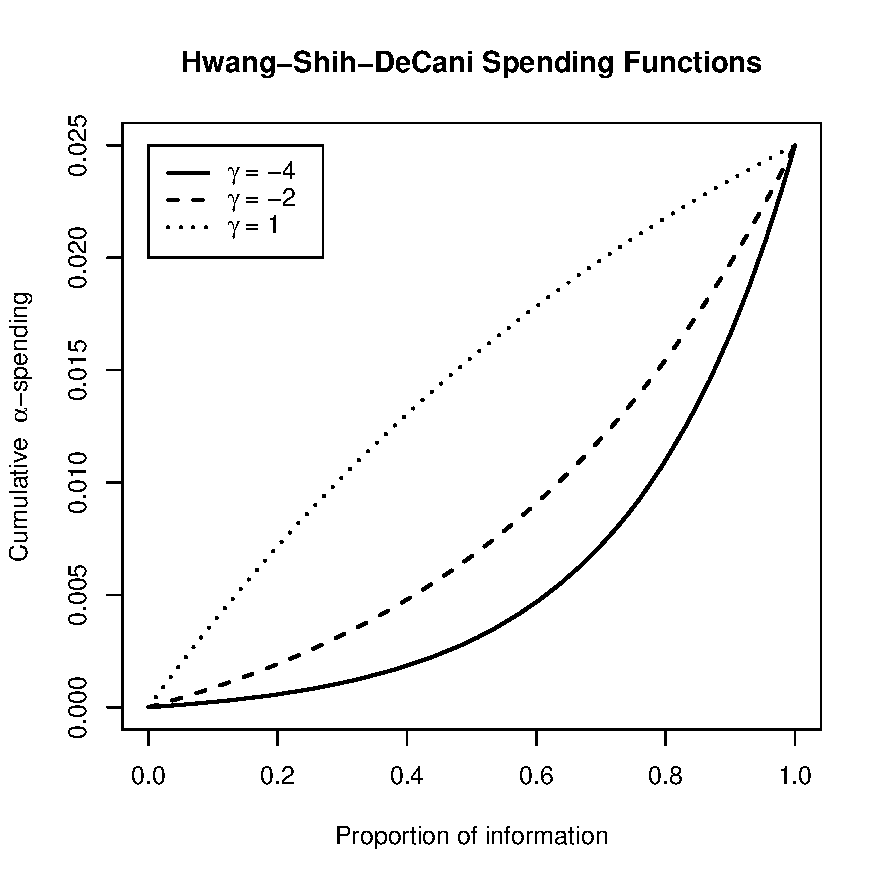
\includegraphics[width=.6\textwidth]{figs/HSDexample.pdf}
\end{center}
\caption{Hwang-Shih-DeCani spending function example\label{fig:hsd}}
\end{figure}%

\end{center}

\subsection{Resetting timing of analyses\label{sec:reset}}

When designed with a spending function, the timing and number of analyses may
be altered during the course of the trial. \ This is very easily handled in
the \texttt{gsDesign()} routine using the input arguments \texttt{n.I} and
\texttt{maxn.IPlan}. We demonstrate this by example. Suppose a trial was
originally designed with the call:

\bigskip

\begin{verbatim}
> x <- gsDesign(k=5, n.fix=800)
> x$upper$bound
> x$n.I
\end{verbatim}

\bigskip

The second and third lines above show the planned upper bounds and sample
sizes at analyses. Suppose that when executed the final interim was skipped,
the first 2 interims were completed on time, the third interim was completed
at 575 patients (instead of 529 as originally planned), the fourth interim was
skipped, and the final analysis was performed after 875 patients (instead of
after 882 as originally planned). The boundaries for the analyses can be
obtained as follows:

\bigskip
\begin{verbatim}
> gsDesign(k=4, n.fix=800, n.I=c(177,353,575,875), maxn.IPlan=x$n.I[x$k])
\end{verbatim}

\bigskip

This design now has slightly higher power (90.4\%) than the originally planned
90\%. This is because the final boundary was lowered relative to the original
plan when the $\alpha$-spending planned for the fourth interim was saved
for the final analysis by skipping the final interim. Note that all of the
arguments for the original design must be supplied when the study is
re-designed---in addition to adding \texttt{n.I}, which may have the same
number, fewer, or more interim analyses compared to the original plan. If the
sample size for the final analysis is changed, \texttt{maxn.IPlan} should be
passed in as the original final sample size in order to appropriately assign
$\alpha$- and $\beta$-spending for the interim analyses.


\section{Advanced spending function details\label{sec:sfDetails}}
\subsection{Spending functions as arguments\label{sec:sfArgs}}
Except for the "OF", "Pocock" and "WT" examples given in Section \ref{sec:boundfam}, a spending function passed to \texttt{gsDesign()} through the arguments \code{sfu} (upper bound) and \code{sfl} (lower bound) must have the following calling sequence:

\bigskip

\texttt{sfname(alpha, t, param)}

\bigskip

where \texttt{sfname} is an arbitrary name for a spending function available
from the package or written by the user. The arguments are as follows:

\begin{itemize}
\item \texttt{alpha}: a real value ($0 < \mathtt{alpha} < 1$).
The total error spending for the boundary to be determined. 
This would be replaced with the following values from a call to \texttt{gsDesign()}:
\texttt{alpha} for the upper bound, and either \texttt{beta} (for
\texttt{test.type = 3} or \texttt{4}) or \texttt{astar} (for 
\texttt{test.type = 5} or \texttt{6}) for the lower bound.

\item \texttt{t}: a vector of arbitrary length $m$ of real values, $0 \leq
t_{1} < t_{2} < \ldots t_{m}\leq1$. 
Specifies the proportion of spending for which values of the spending function are to be computed.

\item \texttt{param}: for all cases here, this is either a real value or a
vector of real values. One or more parameters that (with the parameter
\texttt{alpha}) fully specify the spending function. This is specified in
a call to \texttt{gsDesign()} with \texttt{sfupar} for the upper bound and
\texttt{sflpar} for the lower bound.
\end{itemize}

The value returned is of the class \texttt{spendfn} which was described in 
Section~\ref{sec:spendfn}, The \texttt{spendfn} Class.

The following code and output demomstrate that the default value \texttt{sfHSD} for the upper and lower spending functions \texttt{sfu} and \texttt{sfl} is a function:

\bigskip
\begin{verbatim}
> sfHSD
function (alpha, t, param) 
{
    checkScalar(param, "numeric", c(-40, 40))
    t[t > 1] <- 1
    x <- list(name = "Hwang-Shih-DeCani", param = param, parname = "gamma", 
        sf = sfHSD, spend = if (param == 0) t * alpha else alpha * 
            (1 - exp(-t * param))/(1 - exp(-param)), bound = NULL, 
        prob = NULL)
    class(x) <- "spendfn"
    x
}
<environment: namespace:gsDesign>
\end{verbatim}
\bigskip

Table 1 summarizes many spending functions available in the package. A basic
description of each type of spending function is given. The table begins with
standard spending functions followed by two investigational spending
functions: \texttt{sfExponential()} and \texttt{sfLogistic()}. These spending
functions are discussed further in Section~\ref{sec:invspendfun}, Investigational Spending Functions, but
are included here due to their simple forms. The logistic spending function
represented by \texttt{sfLogistic()} has been used in several trials. It
represents a class of two-parameter spending functions that can provide
flexibility not available from one-parameter families. The
\texttt{sfExponential()} spending function is included here as it provides an
excellent approximation of an O'Brien-Fleming design as follows:

\bigskip

\begin{verbatim}
gsDesign(test.type=2, sfu=sfExponential, sfupar=0.75)
\end{verbatim}
\bigskip

See also subsections below and online documentation of spending functions.

\bigskip

\begin{table}
\caption{Spending function definitions and parameterizations.}
\begin{tabular}
[c]{cccc}\hline
Function & Spending Function & Functional & Parameter\\
(parameter) & Family & Form & (\texttt{sfupar} or \texttt{sflpar})\\\hline
\texttt{sfHSD} & Hwang-Shih- &  & Value in [-40,40).\\
\texttt{\ (gamma)} & DeCani & $\alpha\frac{1-\exp(-\gamma t)}{1-\exp(-\gamma
)}$ & -4=O'Brien-Fleming like;\\
&  &  & 1=Pocock-like\\\hline
\texttt{sfPower} &  &  & Value in $(0,+\infty)$\\
\texttt{(rho)} & Kim-DeMets & $\alpha t^{\rho}$ & 3=O'Brien-Fleming like\\
&  &  & 1=Pocock-like\\\hline
\texttt{sfLDPocock} & Pocock & $\alpha\log(1+(e-1)t)$ & None\\
\texttt{(none)} & approximation &  & \\\hline
\texttt{sfLDOF } & O'Brien-Fleming & $2\left(  1-\Phi\left(  \frac{\Phi
^{-1}(\alpha/2)}{\sqrt{t}}\right)  \right)  $ & None\\
\texttt{(none)} & approximation &  & \\\hline
\texttt{sfLinear} & Piecewise linear & Specified points & Cumulative proportion of\\
\texttt{(t}$_{1}$,\texttt{t}$_{2}$,...,\texttt{t}$_{m}$\texttt{)}
&specification 
& $0<t_{1}\ldots<t_{m}<1$ 
& information and error\\
\texttt{(p}$_{1}$,\texttt{p}$_{2}$,...,\texttt{p}$_{m}$\texttt{)} 
&& $0<p_{1}\ldots<p_{m}<1$
& spending for given timepoints\\\hline
\texttt{sfExponential} &  &  & $(0,10]$\\
\texttt{(nu)} & Exponential & $\alpha^{t^{-\nu}}$ & Recommend $\nu<1$\\
&  &  & $0.75=$O'Brien-Fleming-like\\\hline
\texttt{sfLogistic} & Logistic & $\alpha\frac{e^{a}\left(  \frac{t}
{1-t}\right)  ^{b}}{1+e^{a}\left(  \frac{t}{1-t}\right)  ^{b}}$ & $b>0$\\
\texttt{(a,b)} &  &  & \\\hline
\texttt{"WT"} & Wang-Tsiatis & $C(k,\alpha,\Delta)(i/K)^{\Delta-1/2}$ &
0=O'Brien-Fleming bound\\
\texttt{(Delta)} & bounds &  & 0.5=Pocock bound\\\hline
\texttt{"Pocock"} & Pocock &  & This is a special case\\
\texttt{(none)} & bounds &  & of WT with $\Delta=1/2.$\\\hline
\texttt{"OF"} & O'Brien-Fleming &  & This is a special case\\
\texttt{(none)} & bounds &  & of WT with $\Delta=0.$\\\hline
\end{tabular}
\end{table}

\subsection{Investigational spending functions\label{sec:invspendfun}}

When designing a clinical trial with interim analyses, the rules for stopping
the trial at an interim analysis for a positive or a negative efficacy result
must fit the medical, ethical, regulatory and statistical situation that is
presented. Once a general strategy has been chosen, it is not unreasonable to
discuss precise boundaries at each interim analysis that would be considered
ethical for the purpose of continuing or stopping a trial. Given such
specified boundaries, we discuss here the possibility of numerically fitting
$\alpha$- and $\beta$-spending functions that produce these boundaries.
Commonly-used one-parameter families may not provide an adequate fit to
multiple desired critical values. We present a method of deriving
two-parameter families to provide some additional flexibility along with
examples to demonstrate their usefulness. This method has been found to be
useful in designing multiple trials, including the CAPTURE\ trial
\cite{CAPTURE}, the GUSTO\ V trial \cite{GUSTOV} and three ongoing trials at Merck.

One method of deriving a two-parameter spending function is to use the
incomplete beta distribution which is commonly denoted by $I_{x}(a,b)$ where
$a>0$, $b>0$. We let%
\[
\alpha(t;a,b)=\alpha I_{t}(a,b).
\]
This spending function is implemented in \texttt{sfBetaDist()}; developing
code for this is also demonstrated below in Section~\ref{sec:newspendfn},
Writing Code for a New Spending Function.

Another approach allows fitting spending functions by solving a linear system
of 2 equations in 2 unknowns. A two-parameter family of spending function is
defined using an arbitrary, continuously increasing cumulative distribution
function $F()$ defined on $(-\infty, \infty)$, a real-valued parameter $a$ and
a positive parameter $b$:
\begin{equation}
\alpha(t;a,b)=\alpha F(a+bF^{-1}(t)).\label{2 param sf}%
\end{equation}
Fix two points of the spending function 
$0 < \mathtt{t0} < \mathtt{t1} < 1 $ to have spending function values specified by \texttt{u0} $\times
$ \texttt{alpha} and \texttt{u1} $\times$ \texttt{alpha}, respectively, where 
$0 < \mathtt{u0} < \mathtt{u1} < 1$. Equation (\ref{2 param sf}) now yields two linear equations with two
unknowns, namely for $i=1,2$
\[
F^{-1}(u_{i})=a+bF^{-1}(t_{i}).
\]
The four value specification of \texttt{param} for this family of spending
functions is \texttt{param=c(t0, t1, u0, u1)} where the objective is that
\texttt{sf(t0) = alpha*u0} and \texttt{sf(t1) = alpha*u1}. In this
parameterization, all four values must be between 0 and 1 and 
$\mathtt{t0} < \mathtt{t1}$, $\mathtt{u0} < \mathtt{u1}$.

The logistic distribution has been used with this strategy to
produce spending functions for ongoing trials at Merck Research Laboratories
in addition to the GUSTO V trial \cite{GUSTOV}. The logit function is defined
for $0<u<1$ as ${\rm logit}(u)=\log(u/(1-u))$. Its inverse is defined for
$x\in(-\infty,\infty)$ as ${\rm logit}^{-1}(x)=e^{x}/(1+e^{x})$. Letting $b>0$,
$c=e^{a}>0$, $F(x)={\rm logit}^{-1}(x)$ and applying (\ref{2 param sf}) we obtain
the logistic spending function family:
\begin{align}
\alpha(t;a,b)  & =\alpha\times {\rm logit}^{-1}(\log(c)+b\times
{\rm logit}(u))\label{logistic sf}\\
& =\alpha\frac{c\left(  \frac{t}{1-t}\right)  ^{b}}{1+c\left(  \frac{t}%
{1-t}\right)  ^{b}}%
\end{align}
The logistic spending function is implemented in \texttt{sfLogistic()}.
Functions are also available replacing $F()$ with the cumulative distribution
functions for the standard normal distribution (\texttt{sfNormal()}), two
versions of the extreme value distribution (sfExtremeValue() with
$F(x)=exp(-exp(-x)$) and sfExtremeValue2 with $F(x)=1-exp(-exp(x))$), the
central t-distribution (\texttt{sfTDist()}), and the Cauchy distribution
(\texttt{sfCauchy()}). Of these, \texttt{sfNormal()} is fairly similar to
\texttt{sfLogistic()}. \ On the other hand, \texttt{sfCauchy()} can behave
quite differently. The function \texttt{sfTDist()} provides intermediary
spending functions bounded by \texttt{sfNormal()} and \texttt{sfCauchy()}; it
requires an additional parameter, the degrees of freedom \ See online help for
more complete documentation, particularly for \texttt{sfTDist()}. \ Following
is an example that plots several of these spending functions that fit through
the same two points (\texttt{t1}=0.25, \ \texttt{t2}=0.5, \texttt{u1}=0.1,
\texttt{u2}=0.2) but behave differently for $t>1/2$.

\bigskip

\begin{verbatim}
> plotsf <- function(alpha,t,param)
{
    plot(t, sfCauchy(alpha, t, param)$spend, lwd=2,
         xlab="Proportion of enrollment",
         ylab="Cumulative spending", type="l")
    lines(t, sfLogistic(alpha, t, param)$spend, lty=4, lwd=2)
    lines(t, sfNormal(alpha, t, param)$spend, lty=5, lwd=2)
    lines(t, sfTDist(alpha, t, c(param, 1.5))$spend, lty=2, lwd=2)
    lines(t, sfTDist(alpha, t, c(param,2.5))$spend, lty=3, lwd=2)
    legend(x=c(.0, .3), y=alpha * c(.7,1), lty=1:5, lwd=2,
           legend=c("Cauchy", "t 1.5 df", "t 2.5 df", "Logistic", "Normal"))
}
> t <- 1:199/200
> t <- c(t, .9975, .99875, .9995, .99975)
> param <- c(.25, .5, .1, .2)
> plotsf(.025,t,param)
\end{verbatim}

\begin{center}%
\begin{figure}
\begin{center}
\includegraphics[width=.6\textwidth]{figs/sfLogistic.pdf}
\end{center}
\caption{Example fitting two- and three-parameter spending functions}
\end{figure}%

\end{center}

\subsection{Optimized spending functions}

The following two examples demonstrate some of the flexibility and research
possibilities for the \texttt{gsDesign} package. The particular examples may or may not
be of interest, but the strategy may be applied using a variety of
optimization criteria. First, we consider finding a spending function to match
a Wang-Tsiatis design. This could be useful to adjust a Wang-Tsiatis design if
the timing of interim analyses are not as originally planned. Second, we
replicate a result from Anderson \cite{AndBMJ} which minimized expected value
of the square of sample size over a family of spending functions and a prior distribution.

\begin{example}
Approximating a Wang-Tsiatis design
\end{example}

We have noted several approximations of O'Brien-Fleming and Pocock spending
rules using spending functions in the table above. Following is sample code to
provide a good approximation of Wang-Tsiatis bounds with a given parameter
$\Delta$. \ This includes O'Brien-Fleming ($\Delta$=0) and Pocock ($\Delta
$=0.5) designs. First, we define a function that computes the sum of squared
deviations of the boundaries of a Wang-Tsiatis design compared to a
one-parameter spending function family with a given parameter value of
\texttt{x}. Note that \texttt{Delta} is the parameter for the Wang-Tsiatis
design that we are trying to approximate. Other parameters are as before;
recall that \texttt{test.type} should be limited to 1 or 2 for Wang-Tsiatis
designs. Defaults are used for parameters for \texttt{gsDesign()} not included here.

\bigskip

\begin{verbatim}
WTapprox <- function(x, alpha=0.025, beta=.1, k=3, sf=sfHSD, 
                     Delta=.25, test.type=2)
{
    # Wang-Tsiatis comparison with a one-parameter spending function
    y1 <- gsDesign(k=k, alpha=alpha, beta=beta, test.type=test.type, sfu="WT",
                   sfupar=Delta)$upper$bound
    y2 <- gsDesign(k=k, alpha=alpha, beta=beta, test.type=test.type, sfu=sf,
                   sfupar=x)$upper$bound
    z <- y1-y2
    return(sum(z*z))
}
\end{verbatim}
\bigskip

We consider approximating a two-sided O'Brien-Fleming design with \texttt{alpha}%
=0.025 (one-sided) using the exponential spending function. The function
\texttt{nlminb()} is a standard R function used for minimization. It minimizes
a function passed to it as a function of that function's first 
argument, which may be a vector. The first parameter of \texttt{nlminb()} is 
a starting value for the minimization routine. The second is the function to be
minimized. The parameter \texttt{lower} below provides a lower bound for first
argument to the function being passed to \texttt{nlminb()}. \ Following
parameters are fixed parameters for the function being passed to
\texttt{nlminb()}. The result suggests that for $k=4$, an exponential spending
function with $\nu=0.75$ approximates an O'Brien-Fleming design well.
Examining this same optimization for $k=2$ to 10 suggests that $\nu=0.75$
provides a good approximation of an O'Brien-Fleming design across this range.

\bigskip

\begin{verbatim}
> nu <- nlminb(.67, WTapprox, lower=0, sf=sfExponential, k=4, Delta=0, test.type=2)$par
> nu
[1] 0.7562779
\end{verbatim}
\bigskip

Running comparable code for \texttt{sfHSD()} and \texttt{sfPower()}
illustrates that the exponential spending function can provide a better
approximation of an O'Brien-Fleming design than either the Hwang-Shih-DeCani
or Kim-DeMets spending functions. For Pocock designs, the Hwang-Shih-DeCani
spending function family provides good approximations.

\begin{example}
\bigskip Minimizing the expected value of a power of sample size
\end{example}

In this example, we first define a function that computes a weighted average
across a set of \texttt{theta} values of the expected value of a given power
of the sample size for a design. \ Note that \texttt{sfupar} and
\texttt{sflpar} are specified in the first input argument so that they may later
be optimized using the R routine \texttt{nlminb()}. The code is compact, which
is very nice for writing, but it may be difficult to interpret. A good way to
see how the code works is to define values for all of the parameters and run
each line from the R command prompt, examining the result.

\bigskip

\begin{verbatim}
# Expected value of the power of sample size of a trial 
# as a function of upper and lower spending parameter. 
# Get sfupar from x[1] and sflpar from x[2].
# val is the power of the sample size for which expected
#    values are computed.
# theta is a vector for which expected values are to be computed.
# thetawgt is a vector of the same length used to compute a
#    weighted average of the expected values.
# Other parameters are as for gsDesign.

enasfpar <- function(x, timing=1, theta, thetawgt, k=4, 
                     test.type=4, alpha=0.025, beta=0.1, 
                     astar=0, delta=0, n.fix=1, sfu=sfHSD, 
                     sfl=sfHSD, val=1, tol=0.000001, r=18)
{
    # derive design
    y <- gsDesign(k=k, test.type=test.type, alpha=alpha, beta=beta,
                  astar=astar, delta=delta, n.fix=n.fix, timing=timing,
                  sfu=sfu, sfupar=x[1], sfl=sfl, sflpar=x[2], tol=tol, r=r)
    # compute boundary crossing probabilities for input theta
    y <- gsProbability(theta=theta, d=y)
    # compute sample sizes to the val power
    n <- y$n.I^val
    # compute expected values
    en <- n %*% (y$upper$prob + y$lower$prob)
    # compute weighted average of expected values
    en <- sum(as.vector(en) * as.vector(thetawgt))
    return(en)
}
\end{verbatim}
\bigskip

Now we use this function along with the R routine \texttt{nlminb()} which
finds a minimum across possible values of \texttt{sfupar} and \texttt{sflpar}.
The design derived using the code below and a more extensive discussion can be
found in \cite{AndBMJ}. The code above is more general than in \cite{AndBMJ},
however, as that paper was restricted to \texttt{test.type}=5 (the program
provided there also worked for \texttt{test.type}=6).

\bigskip

\begin{verbatim}
# example from Anderson (2006)
delta <- abs(qnorm(.025) + qnorm(.1))
# use normal distribution to get weights
x <- normalGrid(mu=delta, sigma=delta/2)
x <- nlminb(start=c(.7, -.8), enasfpar, theta=x$z, timing=1, 
       thetawgt=x$wgts, val=2, k=4, test.type=5, tol=0.0000001)
x$message
y <- gsDesign(k=4, test.type=5, sfupar=x$par[1], sflpar=x$par[2])
y
\end{verbatim}

\subsection{Writing code for a new spending function\label{sec:newspendfn}}

Following is sample code using a cumulative distribution function for a
beta-distribution as a spending function. Let B(a,b) denote the complete beta
function. The beta distribution spending function is denoted for any
fixed $a>0$ and $b>0$ by%
\[
\alpha(t)=\frac{\alpha}{B(a,b)}%
%TCIMACRO{\tint \limits_{0}^{t}}%
%BeginExpansion
{\textstyle\int\limits_{0}^{t}}
%EndExpansion
x^{a-1}(1-x)^{b-1}dx.
\]
This spending function provides much of the flexibility of spending functions
in the last subsection, but is not of the same general form. This sample code
is intended to provide guidance in writing code for a new spending function,
if needed.

\bigskip
\begin{verbatim}
# implementation of 2-parameter version of beta distribution spending function
# assumes t and alpha are appropriately specified (does not check!)
sfbdist <- function(alpha, t, param)
{
    # set up return list and its class
    x <- list(name="B-dist example", param=param, parname=c("a","b"), 
         sf=sfbdist, spend=NULL, bound=NULL, prob=NULL, errcode=0, 
         errmsg="No error")
    class(x) <- "spendfn"
    # check for errors in specification of a and b
    # gsReturnError is a simple function available from the 
    # package for saving errors in the returned value}
    if (length(param) != 2) 
    {
        return(gsReturnError(x,errcode=.3,
               errmsg="b-dist example spending function parameter must be of length 2"))
    }
    if (!is.numeric(param)) 
    {
        return(gsReturnError(x,errcode=.1,
               errmsg="Beta distribution spending function parameter must be numeric"))
    }
    if (param[1] <= 0) 
    {
        return(gsReturnError(x,errcode=.12,
               errmsg="1st Beta distribution spending function parameter must be > 0."))
    }
    if (param[2] <= 0) 
    {
        return(gsReturnError(x,errcode=.13,
               errmsg="2nd Beta distribution spending function parameter must be > 0."))
    }
    # set spending using cumulative beta distribution function and return
    x$spend <- alpha * pbeta(t, x$param[1], x$param[2])
    return(x)
}
\end{verbatim}
\bigskip

The flexibility of this spending function is demonstrated by the following
code which produces the plot below. Using a=$\rho$, b=1 produces a Kim-DeMets
spending function $\alpha t^{\rho}$ as shown by the solid line with $\rho$=2.
The dashed line (\texttt{a}=6, \texttt{b}=4) shows a spending function that is
conservative very early, but then aggressive in its spending pattern starting
after about 40\% of data are available. The dotted (\texttt{a}=0.5,
\texttt{b}=0.5) and dot-dashed (\texttt{a}=0.6, \texttt{b}=2) show
increasingly aggressive early spending. These may be useful in setting an
initial high futility bound when the first part of a trial is used as a proof
of concept for a clinical endpoint.

\bigskip

\begin{verbatim}
> # plot some beta distribution spending functions
> plot(0:100/100, sfbdist(1, 0:100/100, c(2,1))$spend, type="l", lwd=2,
+      xlab="Proportion of information",
+      ylab="Cumulative proportion of total spending",
+      main="Beta Distribution Spending Function Example")
> lines(0:100/100, sfbdist(1, 0:100/100, c(6,4))$spend, lty=2, lwd=2)
> lines(0:100/100, sfbdist(1, 0:100/100, c(.5,.5))$spend, lty=3, lwd=2)
> lines(0:100/100, sfbdist(1, 0:100/100, c(.6,2))$spend, lty=4, lwd=2)
> legend(x=c(.65, 1), y=1 * c(0, .25), lty=1:4, lwd=2,
+        legend=c("a=2, b=1", "a=6, b=4", "a=0.5,b=0.5", "a=0.6, b=2"))
\end{verbatim}
\begin{center}%
\begin{figure}
\begin{center}
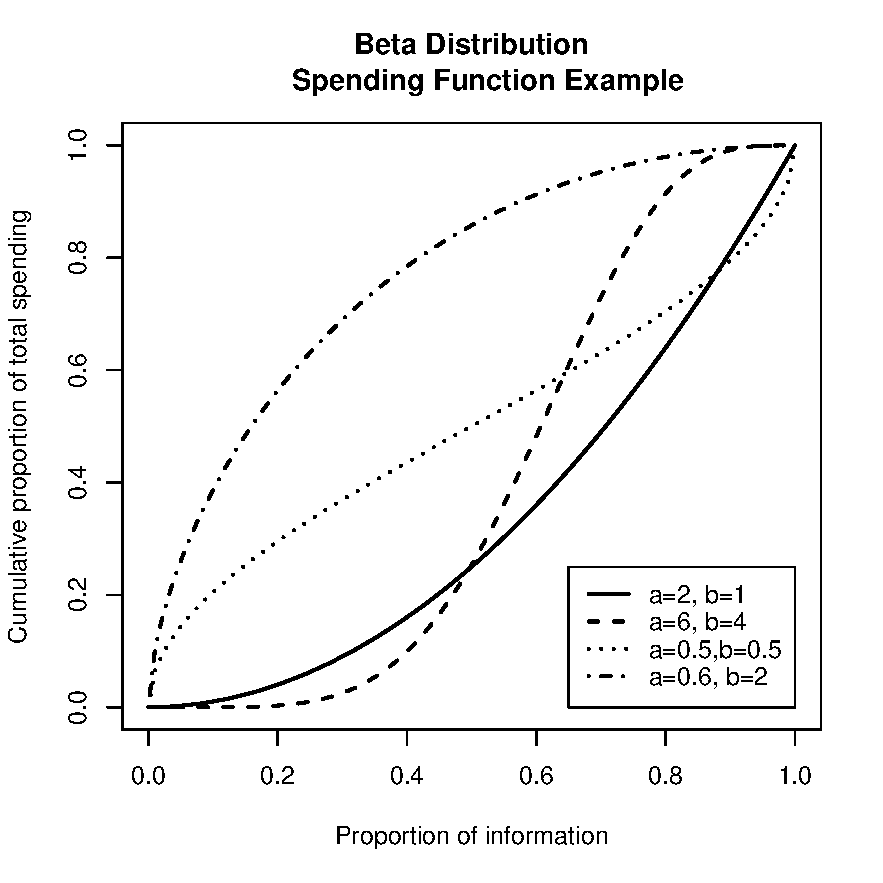
\includegraphics[width=.6\textwidth]{figs/sfbdist.pdf}
\end{center}
\caption{Example plotting user-written beta-distribution spending function}
\end{figure}%
%EndExpansion

\end{center}



\bigskip



\section{Function and Class Reference}
\subsection{gsDesign Package}
\HeaderA{gsDesign-package}{1.0 Group Sequential Design}{gsDesign.Rdash.package}
\keyword{design}{gsDesign-package}
\begin{Description}\relax
gsDesign is a package that derives group sequential designs.
The package allows particular flexibility for designs with alpha- and beta-spending.
Many plots are available for describing design properties.
\end{Description}
\begin{Details}\relax
\Tabular{ll}{
Package: & gsDesign\\
Version: & 1.17.05\\
License: & GPL (version 2 or later)\\
Packaged: & Sun Aug 17 17:41:35 2008; Anderkea\\
Built: & R 2.7.0; i386-pc-mingw32; 2008-08-17 17:41:36; windows\\
}

Index:
\begin{alltt}
gsDesign                2.1: Design Derivation
gsProbability           2.2: Boundary Crossing Probabilities
plot.gsDesign           2.3: Plots for group sequential designs
gsCP                    2.4: Conditional Power Computation
gsBoundCP               2.5: Conditional Power at Interim Boundaries
normalGrid              3.1: Normal Density Grid
MandNtest               3.2: Two-sample binomial sample size
Survival sample size    3.3: Time-to-event sample size calculation
                        (Lachin-Foulkes)
Spending Functions      4.0: Spending functions
sfHSD                   4.1: Hwang-Shih-DeCani Spending Function
sfPower                 4.2: Kim-DeMets (power) Spending Function
sfExponential           4.3: Exponential Spending Function
sfLDPocock              4.4: Lan-DeMets Spending Functions
sfPoints                4.5: Pointwise Spending Function
sfLogistic              4.6: 2-parameter Spending Function Families
sfTDist                 4.7: t-distribution Spending Function
Wang-Tsiatis Bounds     5.0: Wang-Tsiatis Bounds
\end{alltt}
The gsDesign package supports group sequential clinical trial design. 
While there is a strong focus on designs using \eqn{\alpha}{alpha}- and \eqn{\beta}{beta}-spending functions, Wang-Tsiatis designs, 
including O'Brien-Fleming and Pocock designs, are also available.
The ability to design with non-binding futility rules 
controls Type I error in a manner acceptable to regulatory authorities when futility bounds are employed. 

The routines are designed to provide simple access to commonly used designs
using default arguments. 
Standard, published spending functions are supported as well as the ability to write custom spending functions. 
A \code{gsDesign} class is defined and returned by the \code{gsDesign()} function. 
A plot function for this class provides a wide variety of plots: boundaries, power, estimated treatment effect at boundaries, 
conditional power at boundaries, spending function plots, expected sample size plot, and B-values at boundaries.
Using function calls to access the package routines provides a powerful capability to derive designs or output 
formatting that could not be anticipated through a gui interface. 
This enables the user to easily create designs with features they desire, 
such as designs with minimum expected sample size.

Thus, the intent of the gsDesign package is to easily create, fully characterize and even 
optimize routine group sequential trial designs as well as provide a tool to evaluate innovative designs.
\end{Details}
\begin{Author}\relax
Keaven Anderson

Maintainer: Keaven Anderson \code{<keaven\_anderson@merck.com>}
\end{Author}
\begin{References}\relax
Jennison C and Turnbull BW (2000), \emph{Group Sequential Methods with Applications to Clinical Trials}.
Boca Raton: Chapman and Hall.

Proschan, MA, Lan, KKG, Wittes, JT (2006), \emph{Statistical Monitoring of Clinical Trials. A Unified Approach}. 
New York: Springer.
\end{References}
\begin{SeeAlso}\relax
\code{\LinkA{gsDesign}{gsDesign}}, \code{\LinkA{gsProbability}{gsProbability}}
\end{SeeAlso}
\begin{Examples}
\begin{ExampleCode}
# assume a fixed design (no interim) trial with the same endpoint requires 200 subjects
# for 90% power at alpha=.025, one-sided
x <- gsDesign(n.fix=200)
plot(x)
\end{ExampleCode}
\end{Examples}



\subsection{gsDesign main functions}\HeaderA{gsDesign}{2.1: Design Derivation}{gsDesign}
\aliasA{print.gsDesign}{gsDesign}{print.gsDesign}
\keyword{design}{gsDesign}
\begin{Description}\relax
\code{gsDesign()} is used to find boundaries and trial size required for a group sequential design.
\end{Description}
\begin{Usage}
\begin{verbatim}
gsDesign(k=3, test.type=4, alpha=0.025, beta=0.1, astar=0,  
         delta=0, n.fix=1, timing=1, sfu=sfHSD, sfupar=-4,
         sfl=sfHSD, sflpar=-2, tol=0.000001, r=18, n.I = 0,
         maxn.IPlan = 0) 

print.gsDesign(x,...)\end{verbatim}
\end{Usage}
\begin{Arguments}
\begin{ldescription}
\item[\code{k}] Number of analyses planned, including interim and final.
\item[\code{test.type}] \code{1=}one-sided \\
\code{2=}two-sided symmetric \\
\code{3=}two-sided, asymmetric, beta-spending with binding lower bound \\
\code{4=}two-sided, asymmetric, beta-spending with non-binding lower bound \\
\code{5=}two-sided, asymmetric, lower bound spending under the null hypothesis with binding lower bound \\
\code{6=}two-sided, asymmetric, lower bound spending under the null hypothesis with non-binding lower bound. \\ See details, examples and manual.
\item[\code{alpha}] Type I error, always one-sided. Default value is 0.025.
\item[\code{beta}] Type II error, default value is 0.1 (90\% power).
\item[\code{astar}] Normally not specified. If \code{test.type=5} or \code{6}, \code{astar} specifies the total
probability of crossing a lower bound at all analyses combined. 
This will be changed to \eqn{1 - }{}\code{alpha} when default value of 0 is used. 
Since this is the expected usage, normally \code{astar} is not specified by the user.
\item[\code{delta}] Standardized effect size. See details and examples.
\item[\code{n.fix}] Sample size for fixed design with no interim; used to find maximum group sequential sample size.
See details and examples.
\item[\code{timing}] Sets relative timing of interim analyses. Default of 1 produces equally spaced analyses. 
Otherwise, this is a vector of length \code{k} or \code{k-1}.
The values should satisfy \code{0 < timing[1] < timing[2] < ... < timing[k-1] < 
timing[k]=1}.
\item[\code{sfu}] A spending function or a character string indicating a boundary type (that is, \dQuote{WT} for Wang-Tsiatis bounds, \dQuote{OF} for O'Brien-Fleming bounds and \dQuote{Pocock} for Pocock bounds). 
For one-sided and symmetric two-sided testing is used to completely specify spending (\code{test.type=1, 2}), \code{sfu}. 
The default value is \code{sfHSD} which is a Hwang-Shih-DeCani spending function.
See details, \LinkA{Spending function overview}{Spending function overview}, manual and examples.
\item[\code{sfupar}] Real value, default is \eqn{-4}{} which is an O'Brien-Fleming-like conservative bound when used with the default Hwang-Shih-DeCani spending function. This is a real-vector for many spending functions.
The parameter \code{sfupar} specifies any parameters needed for the spending function specified by \code{sfu}; this will be ignored for spending functions (\code{sfLDOF}, \code{sfLDPocock}) 
or bound types (\dQuote{OF}, \dQuote{Pocock}) that do not require parameters.
\item[\code{sfl}] Specifies the spending function for lower boundary crossing probabilities when asymmetric, two-sided testing is performed (\code{test.type = 3}, 
\code{4}, \code{5}, or \code{6}). 
Unlike the upper bound, only spending functions are used to specify the lower bound.
The default value is \code{sfHSD} which is a Hwang-Shih-DeCani spending function.
The parameter \code{sfl} is ignored for one-sided testing (\code{test.type=1}) or symmetric 2-sided testing (\code{test.type=2}). 
See details, spending functions, manual and examples.
\item[\code{sflpar}] Real value, default is \eqn{-2}{}, which, with the default Hwang-Shih-DeCani spending function, 
specifies a less conservative spending rate than the default for the upper bound.
\item[\code{tol}] Tolerance for error (default is 0.000001). Normally this will not be changed by the user.
This does not translate directly to number of digits of accuracy, so use extra decimal places.
\item[\code{r}] Integer value controlling grid for numerical integration as in Jennison and Turnbull (2000); 
default is 18, range is 1 to 80. 
Larger values provide larger number of grid points and greater accuracy.
Normally \code{r} will not be changed by the user.
\item[\code{n.I}] Used for re-setting bounds when timing of analyses changes from initial design; see examples.
\item[\code{maxn.IPlan}] Used for re-setting bounds when timing of analyses changes from initial design; see examples.
\item[\code{x}] In \code{print.gsDesign} this is an object of class gsDesign.
\item[\code{...}] This should allow optional arguments that are standard when calling \code{print}.
\end{ldescription}
\end{Arguments}
\begin{Details}\relax
Many parameters normally take on default values and thus do not require explicit specification.
One- and two-sided designs are supported. Two-sided designs may be symmetric or asymmetric.
Wang-Tsiatis designs, including O'Brien-Fleming and Pocock designs can be generated.
Designs with common spending functions as well as other built-in and user-specified functions for Type I error and 
futility are supported.
Type I error computations for asymmetric designs may assume binding or non-binding lower bounds.
The print function has been extended using \code{print.gsDesign} to print \code{gsDesign} objects; see examples.

The user may ignore the structure of the value returned by \code{gsDesign()} if the standard
printing and plotting suffice; see examples.

\code{delta} and \code{n.fix} are used together to determine what sample size output options the user seeks.
The default, \code{delta=0} and \code{n.fix=1}, results in a \sQuote{generic} design that may be used with any sampling
situation. Sample size ratios are provided and the user multiplies these times the sample size for a fixed design
to obtain the corresponding group sequential analysis times. If \code{delta>0}, \code{n.fix} is ignored, and 
\code{delta} is taken as the standardized effect size - the signal to noise ratio for a single observation;
for example, the mean divided by the standard deviation for a one-sample normal problem. 
In this case, the sample size at each analysis is computed. 
When \code{delta=0} and \code{n.fix>1}, \code{n.fix} is assumed to be the sample size for a fixed design
with no interim analyses. See examples below. 

Following are further comments on the input argument \code{test.type} which is used to control what type of error measurements are used in trial design.
The manual may also be worth some review in order to see actual formulas for boundary crossing probabilities for the various options. 
Options 3 and 5 assume the trial stops if the lower bound is crossed for Type I and Type II error computation (binding lower bound). 
For the purpose of computing Type I error, options 4 and 6 assume the trial continues if the lower bound is crossed (non-binding lower bound); that is a Type I error can be made by crossing an upper bound after crossing a previous lower bound. 
Beta-spending refers to error spending for the lower bound crossing probabilities
under the alternative hypothesis (options 3 and 4).
In this case, the final analysis lower and upper boundaries are assumed to be the same.
The appropriate total beta spending (power) is determined by adjusting the maximum sample size
through an iterative process for all options.
Since options 3 and 4 must compute boundary crossing probabilities under both the null and alternative hypotheses,
deriving these designs can take longer than other options.
Options 5 and 6 compute lower bound spending under the null hypothesis.
\end{Details}
\begin{Value}
An object of the class \code{gsDesign}. This class has the following elements and upon return from 
\code{gsDesign()} contains:
\begin{ldescription}
\item[\code{k}] As input.
\item[\code{test.type}] As input.
\item[\code{alpha}] As input.
\item[\code{beta}] As input.
\item[\code{astar}] As input, except when \code{test.type=5} or \code{6} and \code{astar} is input as 0; in this case
\code{astar} is changed to \code{1-alpha}.
\item[\code{delta}] The standardized effect size for which the design is powered. Will be as input to \code{gsDesign()}
unless it was input as 0; in that case, value will be computed to give desired power for fixed design with input
sample size \code{n.fix}.
\item[\code{n.fix}] Sample size required to obtain desired power when effect size is \code{delta}.
\item[\code{timing}] A vector of length \code{k} containing the portion of the total planned information or sample size at each analysis.
\item[\code{tol}] As input.
\item[\code{r}] As input.
\item[\code{upper}] Upper bound spending function, boundary and boundary crossing probabilities under the NULL and
alternate hypotheses. See \LinkA{Spending function overview}{Spending function overview} and manual for further details.
\item[\code{lower}] Lower bound spending function, boundary and boundary crossing probabilities at each analysis.
Lower spending is under alternative hypothesis (beta spending) for \code{test.type=3} or \code{4}. 
For \code{test.type=2}, \code{5} or \code{6}, lower spending is under the null hypothesis.
For \code{test.type=1}, output value is \code{NULL}. See \LinkA{Spending function overview}{Spending function overview} and manual.
\item[\code{n.I}] Vector of length \code{k}. If values are input, same values are output.
Otherwise, \code{n.I} will contain the sample size required at each analysis 
to achieve desired \code{timing} and \code{beta} for the output value of \code{delta}. 
If \code{delta=0} was input, then this is the sample size required for the specified group sequential design when a fixed design requires a sample size of \code{n.fix}.
If \code{delta=0} and \code{n.fix=1} then this is the relative sample size compared to a fixed design; see details and examples.
\item[\code{maxn.IPlan}] As input.
\end{ldescription}
\end{Value}
\begin{Note}\relax
The manual is not linked to this help file, but is available in library/gsdesign/doc/gsDesignManual.pdf
in the directory where R is installed.
\end{Note}
\begin{Author}\relax
Keaven Anderson \email{keaven\_anderson@merck.}
\end{Author}
\begin{References}\relax
Jennison C and Turnbull BW (2000), \emph{Group Sequential Methods with Applications to Clinical Trials}.
Boca Raton: Chapman and Hall.
\end{References}
\begin{SeeAlso}\relax
\LinkA{gsDesign package overview}{gsDesign package overview}, \LinkA{Plots for group sequential designs}{Plots for group sequential designs}, \code{\LinkA{gsProbability}{gsProbability}}, 
\LinkA{Spending function overview}{Spending function overview}, \LinkA{Wang-Tsiatis Bounds}{Wang.Rdash.Tsiatis Bounds}
\end{SeeAlso}
\begin{Examples}
\begin{ExampleCode}
#  symmetric, 2-sided design with O'Brien-Fleming-like boundaries
#  lower bound is non-binding (ignored in Type I error computation)
#  sample size is computed based on a fixed design requiring n=800
x <- gsDesign(k=5, test.type=2, n.fix=800)

# note that "x" below is equivalent to print(x) and print.gsDesign(x)
x
plot(x)
plot(x, plottype=2)

# Assuming after trial was designed actual analyses occurred after
# 300, 600, and 860 patients, reset bounds 
y <- gsDesign(k=3, test.type=2, n.fix=800, n.I=c(300,600,860),
   maxn.IPlan=x$n.I[x$k])
y

#  asymmetric design with user-specified spending that is non-binding
#  sample size is computed relative to a fixed design with n=1000
sfup <- c(.033333, .063367, .1)
sflp <- c(.25, .5, .75)
timing <- c(.1, .4, .7)
x <- gsDesign(k=4, timing=timing, sfu=sfPoints, sfupar=sfup, sfl=sfPoints,
                    sflpar=sflp,n.fix=1000) 
x
plot(x)
plot(x, plottype=2)

# same design, but with relative sample sizes
gsDesign(k=4, timing=timing, sfu=sfPoints, sfupar=sfup, sfl=sfPoints,
sflpar=sflp)
\end{ExampleCode}
\end{Examples}


\HeaderA{gsProbability}{2.2: Boundary Crossing Probabilities}{gsProbability}
\aliasA{print.gsProbability}{gsProbability}{print.gsProbability}
\keyword{design}{gsProbability}
\begin{Description}\relax
Computes power/Type I error and expected sample size for a group sequential design
across a selected set of parameter values for a given set of analyses and boundaries.
The print function has been extended using \code{print.gsProbability} to print \code{gsProbability} objects; see examples.
\end{Description}
\begin{Usage}
\begin{verbatim}
gsProbability(k=0, theta, n.I, a, b, r=18, d=NULL)
\end{verbatim}
\end{Usage}
\begin{Arguments}
\begin{ldescription}
\item[\code{k}] Number of analyses planned, including interim and final.
\item[\code{theta}] Vector of standardized effect sizes for which boundary crossing probabilities are to be computed.
\item[\code{n.I}] Sample size or relative sample size at analyses; vector of length k. See \code{\LinkA{gsDesign}{gsDesign}} and manual.
\item[\code{a}] Lower bound cutoffs (z-values) for futility or harm at each analysis, vector of length k.
\item[\code{b}] Upper bound cutoffs (z-values) for futility at each analysis; vector of length k.
\item[\code{r}] Control for grid as in Jennison and Turnbull (2000); default is 18, range is 1 to 80.
Normally this will not be changed by the user.
\item[\code{d}] If not \code{NULL}, this should be an object of type \code{gsDesign} returned by a call to \code{gsDesign()}. 
When this is specified, the values of \code{k}, \code{n.I}, \code{a}, \code{b}, and \code{r} will be obtained from \code{d} and
only \code{theta} needs to be specified by the user.
\end{ldescription}
\end{Arguments}
\begin{Details}\relax
Depending on the calling sequence, an object of class \code{gsProbability} or class \code{gsDesign} is returned.
If it is of class \code{gsDesign} then the members of the object will be the same as described in \code{\LinkA{gsDesign}{gsDesign}}.
If \code{d} is input as \code{NULL} (the default), all other arguments (other than \code{r}) must be specified 
and an object of class \code{gsProbability} is returned.
If \code{d} is passed as an object of class \code{gsProbability} or \code{gsDesign} the only other argument required is \code{theta};
the object returned has the same class as the input \code{d}.
On output, the values of \code{theta} input to \code{gsProbability} will be the parameter values for which the
design is characterized.
\end{Details}
\begin{Value}
\begin{ldescription}
\item[\code{k}] As input.
\item[\code{theta}] As input.
\item[\code{n.I}] As input.
\item[\code{lower}] A list containing two elements: \code{bound} is as input in \code{a} and \code{prob} is a matrix of boundary 
crossing probabilities. Element \code{i,j} contains the boundary crossing probability at analysis \code{i} for the \code{j}-th
element of \code{theta} input. All boundary crossing is assumed to be binding for this computation; 
that is, the trial must stop if a boundary is crossed.
\item[\code{upper}] An list of the same form as \code{lower} containing the upper bound and upper boundary crossing probabilities.
\item[\code{en}] A vector of the same length as \code{theta} containing expected sample sizes for the trial design
corresponding to each value in the vector \code{theta}.
\item[\code{r}] As input.
\end{ldescription}
\end{Value}
\begin{Note}\relax
The manual is not linked to this help file, but is available in library/gsdesign/doc/manual.pdf
in the directory where R is installed.
\end{Note}
\begin{Author}\relax
Keaven Anderson \email{keaven\_anderson@merck.com}, Jennifer Sun, John Zhang
\end{Author}
\begin{References}\relax
Jennison C and Turnbull BW (2000), \emph{Group Sequential Methods with Applications to Clinical Trials}.
Boca Raton: Chapman and Hall.
\end{References}
\begin{SeeAlso}\relax
\LinkA{Group Sequential Plots}{Group Sequential Plots}, \code{\LinkA{gsDesign}{gsDesign}}, \LinkA{gsDesign-package}{gsDesign.Rdash.package}
\end{SeeAlso}
\begin{Examples}
\begin{ExampleCode}
# making a gsDesign object first may be easiest...
x <- gsDesign()

# take a look at it
x

# default plot for gsDesign object shows boundaries
plot(x)

# plottype=2 shows boundary crossing probabilities
plot(x, plottype=2)

# now add boundary crossing probabilities and 
# expected sample size for more theta values
y <- gsProbability(d=x, theta=x$delta*seq(0, 2, .25))
class(y)

# note that "y" below is equivalent to print(y) and print.gsProbability(y)
y

# the plot does not change from before since this is a gsDesign object
# note that theta/delta is on x axis
plot(y, plottype=2)

# now let's see what happens with a gsProbability object
z <- gsProbability(k=3, a=x$lower$bound, b=x$upper$bound, n.I=x$n.I, 
    theta=x$delta*seq(0, 2, .25))

# with the above form,  the results is a gsProbability object
class(z)
z

# default plottype is now 2
# this is the same range for theta,  but plot now has theta on x axis
plot(z)
\end{ExampleCode}
\end{Examples}


\HeaderA{plot.gsDesign}{2.3: Plots for group sequential designs}{plot.gsDesign}
\aliasA{plot.gsProbability}{plot.gsDesign}{plot.gsProbability}
\aliasA{Plots for group sequential designs}{plot.gsDesign}{Plots for group sequential designs}
\keyword{design}{plot.gsDesign}
\begin{Description}\relax
The \code{plot()} function has been extended to work with objects returned by \code{gsDesign()} and \code{gsProbability()}. 
For objects of type \code{gsDesign}, seven types of plots are provided: z-values at boundaries (default), power, 
estimated treatment effects at boundaries, 
conditional power at boundaries, spending functions, expected sample size, and B-values at boundaries.
For objects of type \code{gsProbability} plots are available for z-values at boundaries, power (default), estimated treatment effects at boundaries, conditional power, expected sample size and B-values at boundaries.
\end{Description}
\begin{Usage}
\begin{verbatim}
plot.gsProbability(x, plottype=2, ...)
plot.gsDesign(x, plottype=1, ...)
\end{verbatim}
\end{Usage}
\begin{Arguments}
\begin{ldescription}
\item[\code{x}] Object of class \code{gsDesign} for \code{plot.gsDesign()} or \code{gsProbability} for 

\code{plot.gsProbability()}.
\item[\code{plottype}] 1=boundary plot (default for \code{gsDesign}),

2=power plot (default for \code{gsProbability}), 

3=estimated treatment effect at boundaries, 

4=conditional power at boundaries, 

5=spending function plot 
(only available if \code{class(x)=="gsDesign"}), 

6=expected sample size plot, and 

7=B-values at boundaries. 

Character values for \code{plottype} may also be entered: \code{"Z"} for plot
type 1,
\code{"power"} for plot type 2, \code{"thetahat"} for plot type 3,
\code{"CP"} for plot type 4, \code{"sf"} for plot type 5, \code{"ASN"}, 
\code{"N"} or \code{"n"} for plot type 6, and \code{"B"}, \code{"B-val"} or 
\code{"B-value"} for plot type 7.
\item[\code{...}] This allows many optional arguments that are standard when calling \code{plot}.

Other arguments include: 

\code{theta} which is used for \code{plottype=2}, \code{4}, \code{6}; normally defaults will be adequate; see details. 

\code{ses=TRUE} which applies only when \code{plottype=3} and 

\code{class(x)=="gsDesign"}; indicates that estimated standardized effect size
at the boundary is to be plotted rather than the actual estimate.

\code{xval="Default"} which is only effective when \code{plottype=2} or \code{6}. Appropriately scaled (reparameterized) values for x-axis for power and expected sample size graphs; see details.
\end{ldescription}
\end{Arguments}
\begin{Details}\relax
The intent is that many standard \code{plot()} parameters will function as expected; exceptions to this rule exist.
In particular, \code{main, xlab, ylab, lty, col, lwd, type, pch, cex} have been tested and work for most values of \code{plottype}; one
exception is that \code{type="l"} cannot be overridden when \code{plottype=2}. Default values for labels depend on \code{plottype} and 
the class of \code{x}.

Note that there is some special behavior for values plotted and returned 
for power and expected sample size (ASN) plots for a \code{gsDesign} object.
A call to \code{x<-gsDesign()} produces power and expected sample size for only two \code{theta} values: 0 and \code{x\$delta}. 
The call \code{plot(x, plottype="Power")} (or \code{plot(x,plottype="ASN"}) for a \code{gsDesign} object produces power (expected sample size) curves and returns a \code{gsDesign} object with \code{theta} values determined as follows. 
If \code{theta} is non-null on input, the input value(s) are used.
Otherwise, for a \code{gsProbability} object, the \code{theta} values from that object are used.
For a \code{gsDesign} object where \code{theta} is input as \code{NULL} (the default), \code{theta=seq(0,2,.05)*x\$delta}) is used. 
For a \code{gsDesign} object, the x-axis values are rescaled to \code{theta/x\$delta} and the label for the x-axis \eqn{theta / delta}{}.
For a \code{gsProbability} object, the values of \code{theta} are plotted and are labeled as \eqn{theta}{}.
See examples below.

Estimated treatment effects at boundaries are computed dividing the Z-values at the boundaries by the square root of \code{n.I} at that analysis. 

Spending functions are plotted for a continuous set of values from 0 to 1. 
This option should not be used if a boundary is used or a pointwise spending function is used
(\code{sfu} or \code{sfl="WT", "OF", "Pocock"} or \code{sfPoints}). 

Conditional power is computed using the function \code{gsBoundCP()}. 
The default input for this routine is \code{theta="thetahat"} which will compute the conditional power at each bound using the estimated treatment effect at that bound. 
Otherwise, if the input is \code{gsDesign} object conditional power is computed assuming \code{theta=x\$delta}, the original effect size for which the trial was planned.

Average sample number/expected sample size is computed using \code{n.I} at each analysis times the probability of crossing a boundary at that analysis.
If no boundary is crossed at any analysis, this is counted as stopping at the final analysis.

B-values are Z-values multiplied by \code{sqrt(t)=sqrt(x\$n.I/n\$n.I[x\$k])}. 
Thus, the expected value of a B-value at an analysis is the true value of 
\eqn{theta}{} multiplied by the proportion of total planned observations at that time.
See Proschan, Lan and Wittes (2006).
\end{Details}
\begin{Value}
An object of \code{class(x)}; in many cases this is the input value of \code{x}, while in others \code{x\$theta} is replaced 
and corresponding characteristics computed; see details.
\end{Value}
\begin{Note}\relax
The manual is not linked to this help file, but is available in library/gsdesign/doc/gsDesignManual.pdf
in the directory where R is installed.
\end{Note}
\begin{Author}\relax
Keaven Anderson \email{keaven\_anderson@merck.com}
\end{Author}
\begin{References}\relax
Jennison C and Turnbull BW (2000), \emph{Group Sequential Methods with Applications to Clinical Trials}.
Boca Raton: Chapman and Hall.

Proschan, MA, Lan, KKG, Wittes, JT (2006), \emph{Statistical Monitoring of Clinical Trials. A Unified Approach}. 
New York: Springer.
\end{References}
\begin{SeeAlso}\relax
\LinkA{gsDesign package overview}{gsDesign package overview}, \code{\LinkA{gsDesign}{gsDesign}}, \code{\LinkA{gsProbability}{gsProbability}}
\end{SeeAlso}
\begin{Examples}
\begin{ExampleCode}
#  symmetric, 2-sided design with O'Brien-Fleming-like boundaries
#  lower bound is non-binding (ignored in Type I error computation)
#  sample size is computed based on a fixed design requiring n=100
x <- gsDesign(k=5, test.type=2, n.fix=100)
x

# the following translate to calls to plot.gsDesign since x was
# returned by gsDesign; run these commands one at a time
plot(x)
plot(x, plottype=2)
plot(x, plottype=3)
plot(x, plottype=4)
plot(x, plottype=5)
plot(x, plottype=6)
plot(x, plottype=7)

#  choose different parameter values for power plot
#  start with design in x from above
y <- gsProbability(k=5, theta=seq(0, .5, .025), x$n.I,
                   x$lower$bound, x$upper$bound)

# the following translates to a call to plot.gsProbability since
# y has that type
plot(y)
\end{ExampleCode}
\end{Examples}


\HeaderA{gsCP}{2.4: Conditional Power Computation}{gsCP}
\keyword{design}{gsCP}
\begin{Description}\relax
\code{gsCP()} takes a given group sequential design, assumes an interim z-statistic 
at a specified interim analysis and computes boundary crossing probabilities at future planned analyses.
\end{Description}
\begin{Usage}
\begin{verbatim}
gsCP(x, theta=NULL, i=1, zi=0, r=18)
\end{verbatim}
\end{Usage}
\begin{Arguments}
\begin{ldescription}
\item[\code{x}] An object of type \code{gsDesign} or \code{gsProbability}
\item[\code{theta}] \eqn{\theta}{theta} value(s) at which conditional power is to be computed; if \code{NULL}, 
an estimated value of \eqn{\theta}{theta} based on the interim test statistic (\code{zi/sqrt(x\$n.I[i])}) as well as at \code{x\$theta}
is computed.
\item[\code{i}] analysis at which interim z-value is given
\item[\code{zi}] interim z-value at analysis i
\item[\code{r}] Integer value controlling grid for numerical integration as in Jennison and Turnbull (2000); 
default is 18, range is 1 to 80. 
Larger values provide larger number of grid points and greater accuracy.
Normally \code{r} will not be changed by the user.
\end{ldescription}
\end{Arguments}
\begin{Details}\relax
See Statistical Methods section of manual for further clarification. See also Muller and Schaffer (2001) for background theory.
\end{Details}
\begin{Value}
An object of the class \code{gsProbability}.
Based on the input design and the interim test statistic, the output object has bounds for test statistics
computed based on observations after interim \code{i} that are equivalent to the original design crossing boundaries conditional
on the interim test statistic value input. 
Boundary crossing probabilities are computed for the input 
\eqn{\theta}{theta} values.
\end{Value}
\begin{Note}\relax
The manual is not linked to this help file, but is available in library/gsdesign/doc/manual.pdf
in the directory where R is installed.
\end{Note}
\begin{Author}\relax
Keaven Anderson \email{keaven\_anderson@merck.com}, Jennifer Sun, John Zhang
\end{Author}
\begin{References}\relax
Jennison C and Turnbull BW (2000), \emph{Group Sequential Methods with Applications to Clinical Trials}.
Boca Raton: Chapman and Hall.

Muller, Hans-Helge and Schaffer, Helmut (2001), Adaptive group sequential designs for clinical trials:
combining the advantages of adaptive and classical group sequential approaches. \emph{Biometrics};57:886-891.
\end{References}
\begin{SeeAlso}\relax
\code{\LinkA{gsDesign}{gsDesign}}, \code{\LinkA{gsProbability}{gsProbability}}, \code{\LinkA{gsBoundCP}{gsBoundCP}}
\end{SeeAlso}
\begin{Examples}
\begin{ExampleCode}
# set up a group sequential design
x <- gsDesign(k=5)
x

# assuming a z-value of .5 at analysis 2, what are conditional 
# boundary crossing probabilities for future analyses
# assuming theta values from x as well as a value based on the interim
# observed z
CP <- gsCP(x, i=2, zi=.5)
CP

# summing values for crossing future upper bounds gives overall
# conditional power for each theta value
CP$theta
CP$upper$prob 
\end{ExampleCode}
\end{Examples}


\HeaderA{gsBoundCP}{2.5: Conditional Power at Interim Boundaries}{gsBoundCP}
\keyword{design}{gsBoundCP}
\begin{Description}\relax
\code{gsBoundCP()} computes the total probability of crossing future upper bounds
given an interim test statistic at an interim bound.
For each interim boundary
assumes an interim test statistic at the boundary and
computes the probability of crossing any of the later upper boundaries.
\end{Description}
\begin{Usage}
\begin{verbatim}
gsBoundCP(x, theta="thetahat", r=18)
\end{verbatim}
\end{Usage}
\begin{Arguments}
\begin{ldescription}
\item[\code{x}] An object of type \code{gsDesign} or \code{gsProbability}
\item[\code{theta}] if \code{"thetahat"} and \code{class(x)!="gsDesign"}), conditional power computations for
each boundary value are computed using estimated treatment effect assuming a test statistic at that boundary
(\code{zi/sqrt(x\$n.I[i]} at analysis \code{i}, interim test statistic \code{zi} and interim 
sample size/statistical information of \code{x\$n.I[i]}). Otherwise, conditional power is computed
assuming the input scalar value \code{theta}.

\item[\code{r}] Integer value controlling grid for numerical integration as in Jennison and Turnbull (2000); 
default is 18, range is 1 to 80. 
Larger values provide larger number of grid points and greater accuracy.
Normally \code{r} will not be changed by the user.
\end{ldescription}
\end{Arguments}
\begin{Details}\relax
See Statistical Methods section of manual for further clarification. See also Muller and Schaffer (2001) for background theory.
\end{Details}
\begin{Value}
A list containing two vectors, \code{CPlo} and \code{CPhi}.
\begin{ldescription}
\item[\code{CPlo}] A vector of length \code{x\$k-1} with conditional powers of crossing upper bounds
given interim test statistics at each lower bound
\end{ldescription}

\code{CPhi}{A vector of length \code{x\$k-1} with conditional powers of crossing upper bounds
given interim test statistics at each upper bound.}
\end{Value}
\begin{Note}\relax
The manual is not linked to this help file, but is available in library/gsdesign/doc/manual.pdf
in the directory where R is installed.
\end{Note}
\begin{Author}\relax
Keaven Anderson \email{keaven\_anderson@merck.com}, Jennifer Sun, John Zhang
\end{Author}
\begin{References}\relax
Jennison C and Turnbull BW (2000), \emph{Group Sequential Methods with Applications to Clinical Trials}.
Boca Raton: Chapman and Hall.

Muller, Hans-Helge and Schaffer, Helmut (2001), Adaptive group sequential designs for clinical trials:
combining the advantages of adaptive and classical group sequential approaches. \emph{Biometrics};57:886-891.
\end{References}
\begin{SeeAlso}\relax
\code{\LinkA{gsDesign}{gsDesign}}, \code{\LinkA{gsProbability}{gsProbability}}, \code{\LinkA{gsCP}{gsCP}}
\end{SeeAlso}
\begin{Examples}
\begin{ExampleCode}
# set up a group sequential design
x <- gsDesign(k=5)
x

# compute conditional power based on interim treatment effects
gsBoundCP(x)

# compute conditional power based on original x$delta
gsBoundCP(x, theta=x$delta)
\end{ExampleCode}
\end{Examples}


\HeaderA{gsBound}{2.6: Boundary derivation - low level}{gsBound}
\aliasA{gsBound1}{gsBound}{gsBound1}
\keyword{design}{gsBound}
\begin{Description}\relax
\code{gsBound()} and \code{gsBound1()} are lower-level functions used to find boundaries for a group sequential design.
They are not recommended (especially \code{gsBound1()}) for casual users.
These functions do not adjust sample size as \code{gsDesign()} does to ensure appropriate power for a design.

\code{gsBound()} computes upper and lower bounds given boundary crossing probabilities assuming a mean of 0, the usual null hypothesis.
\code{gsBound1()} computes the upper bound given a lower boundary, upper boundary crossing probabilities and an arbitrary mean (\code{theta}).
\end{Description}
\begin{Usage}
\begin{verbatim}
gsBound(I, trueneg, falsepos, tol=0.000001, r=18)
gsBound1(theta, I, a, probhi, tol=0.000001, r=18, printerr=0)
\end{verbatim}
\end{Usage}
\begin{Arguments}
Note that all vector arguments should have the same length which will be denoted here as \code{k}.
\begin{ldescription}
\item[\code{theta}] Scalar containing mean (drift) per unit of statistical information.
\item[\code{I}] Vector containing statistical information planned at each analysis.
\item[\code{a}] Vector containing lower bound that is fixed for use in \code{gsBound1}.
\item[\code{trueneg}] Vector of desired probabilities for crossing upper bound assuming mean of 0.
\item[\code{falsepos}] Vector of desired probabilities for crossing lower bound assuming mean of 0.
\item[\code{probhi}] Vector of desired probabilities for crossing upper bound assuming mean of theta.
\item[\code{tol}] Tolerance for error (scalar; default is 0.000001). Normally this will not be changed by the user.
This does not translate directly to number of digits of accuracy, so use extra decimal places.
\item[\code{r}] Single integer value controlling grid for numerical integration as in Jennison and Turnbull (2000); 
default is 18, range is 1 to 80. 
Larger values provide larger number of grid points and greater accuracy.
Normally \code{r} will not be changed by the user.
\item[\code{printerr}] If this scalar argument set to 1, this will print messages from underlying C program.
Mainly intended to notify user when an output solution does not match input specifications.
This is not intended to stop execution as this often occurs when deriving a design in \code{gsDesign}
that uses beta-spending.
\end{ldescription}
\end{Arguments}
\begin{Details}\relax
The function \code{gsBound1()} requires special attention to detail and knowledge of behavior when a design corresponding to the input parameters does not exist.
\end{Details}
\begin{Value}
Both routines return a list. Common items returned by the two routines are: 
\begin{ldescription}
\item[\code{k}] The length of vectors input; a scalar.
\item[\code{theta}] As input in \code{gsBound1()}; 0 for \code{gsBound()}.
\item[\code{I}] As input.
\item[\code{a}] For \code{gsbound1}, this is as input. For \code{gsbound} this is the derived lower boundary required to yield the input boundary crossing probabilities under the null hypothesis.
\item[\code{b}] The derived upper boundary required to yield the input boundary crossing probabilities under the null hypothesis.
\item[\code{tol}] As input.
\item[\code{r}] As input.
\item[\code{error}] Error code. 0 if no error; greater than 0 otherwise.
\item[\code{rates}] a list containing two items:
\item[\code{falsepos}] vector of upper boundary crossing probabilities as input.
\item[\code{trueneg}] vector of lower boundary crossing probabilities as input.
\item[\code{problo}] vector of lower boundary crossing probabilities; computed using input lower bound and derived upper bound.
\item[\code{probhi}] vector of upper boundary crossing probabilities as input.
\end{ldescription}
\end{Value}
\begin{Note}\relax
The manual is not linked to this help file, but is available in library/gsdesign/doc/gsDesignManual.pdf
in the directory where R is installed.
\end{Note}
\begin{Author}\relax
Keaven Anderson \email{keaven\_anderson@merck.}
\end{Author}
\begin{References}\relax
Jennison C and Turnbull BW (2000), \emph{Group Sequential Methods with Applications to Clinical Trials}.
Boca Raton: Chapman and Hall.
\end{References}
\begin{SeeAlso}\relax
\LinkA{gsDesign package overview}{gsDesign package overview}, \code{\LinkA{gsDesign}{gsDesign}}, \code{\LinkA{gsProbability}{gsProbability}}
\end{SeeAlso}
\begin{Examples}
\begin{ExampleCode}
# set boundaries so that probability is .01 of first crossing
# each upper boundary and .02 of crossing each lower boundary
# under the null hypothesis
x <- gsBound(I=c(1, 2, 3)/3, trueneg=array(.02, 3),
             falsepos=array(.01, 3))
x

#  use gsBound1 to set up boundary for a 1-sided test
x <- gsBound1(theta= 0, I=c(1, 2, 3) / 3, a=array(-20, 3),
              probhi=c(.001, .009, .015))
x$b

# check boundary crossing probabilities with gsProbability 
y <- gsProbability(k=3, theta=0, n.I=x$I, a=x$a, b=x$b)$upper$prob

#  Note that gsBound1 only computes upper bound 
#  To get a lower bound under a parameter value theta:
#      use minus the upper bound as a lower bound
#      replace theta with -theta
#      set probhi as desired lower boundary crossing probabilities 
#  Here we let set lower boundary crossing at 0.05 at each analysis
#  assuming theta=2.2 
y <- gsBound1(theta=-2.2, I=c(1, 2, 3)/3, a= -x$b, 
              probhi=array(.05, 3))
y$b

#  Now use gsProbability to look at design
#  Note that lower boundary crossing probabilities are as
#  specified for theta=2.2, but for theta=0 the upper boundary
#  crossing probabilities are smaller than originally specified
#  above after first interim analysis
gsProbability(k=length(x$b), theta=c(0, 2.2), n.I=x$I, b=x$b, a= -y$b)
\end{ExampleCode}
\end{Examples}



\subsection{Binomial trial functions}\HeaderA{normalGrid}{3.1: Normal Density Grid}{normalGrid}
\keyword{design}{normalGrid}
\begin{Description}\relax
normalGrid() is intended to be used for computation of the expected value of 
a function of a normal random variable.
The function produces grid points and weights to be used for numerical integration.
\end{Description}
\begin{Usage}
\begin{verbatim}
normalGrid(r=18, bounds=c(0,0), mu=0, sigma=1)
\end{verbatim}
\end{Usage}
\begin{Arguments}
\begin{ldescription}
\item[\code{r}] Control for grid points as in Jennison and Turnbull (2000), Chapter 19; default is 18. Range: 1 to 80.
This might be changed by the user (e.g., \code{r=6} which produces 65 gridpoints compare to 185 points when \code{r=18})
when speed is more important than precision.
\item[\code{bounds}] Range of integration. Real-valued vector of length 2. Default value of 0, 0 produces a range 
of + or - 6 standard deviations (6*sigma) from the mean (=mu).
\item[\code{mu}] Mean of the desired normal distribution.
\item[\code{sigma}] Standard deviation of the desired normal distribution.
\end{ldescription}
\end{Arguments}
\begin{Value}
\begin{ldescription}
\item[\code{z}] Grid points for numerical integration.
\item[\code{wgts}] Weights to be used with grid points in \code{z}.
\end{ldescription}
\end{Value}
\begin{Note}\relax
The manual is not linked to this help file, but is available in library/gsdesign/doc/gsDesignManual.pdf
in the directory where R is installed.
\end{Note}
\begin{Author}\relax
Keaven Anderson \email{keaven\_anderson@merck.com}
\end{Author}
\begin{References}\relax
Jennison C and Turnbull BW (2000), \emph{Group Sequential Methods with Applications to Clinical Trials}.
Boca Raton: Chapman and Hall.
\end{References}
\begin{Examples}
\begin{ExampleCode}
#  standard normal distribution
x <- normalGrid(r=3)
plot(x$z, x$wgts)

#  verify that numerical integration replicates sigma
#  get grid points and weights
x <- normalGrid(mu=2, sigma=3)

# compute squared deviation from mean for grid points
dev <- (x$z-2)^2

# multiply squared deviations by integration weights and sum 
sigma2 <- sum(dev * x$wgts)

# square root of sigma2 should be sigma (3)
sqrt(sigma2)

# do it again with larger r to increase accuracy
x <- normalGrid(r=22, mu=2, sigma=3)
sqrt(sum((x$z-2)^2 * x$wgts))

# find expected sample size for default design with
# n.fix=1000
x <- gsDesign(n.fix=1000)
x

y <- normalGrid(r=3, mu=x$theta[2], sigma=x$theta[2] / 1.5)
z <- gsProbability(k=3, theta=y$z, n.I=x$n.I, a=x$lower$bound,
                   b=x$upper$bound)
z <- gsProbability(d=x, theta=y$z)
cat("Expected sample size averaged over normal ")
cat("prior distribution for theta with mu=", 
   x$theta[2], "sigma=", x$theta[2]/1.5, ":",
   round(sum(z$en*y$wgt), 1), "\n")
plot(y$z, z$en, xlab="theta", ylab="E{N}", 
   main="Expected sample size for different theta values")
\end{ExampleCode}
\end{Examples}


\HeaderA{Binomial}{3.2: Testing, Confidence Intervals and Sample Size for Comparing Two Binomial Rates}{Binomial}
\aliasA{ciBinomial}{Binomial}{ciBinomial}
\aliasA{nBinomial}{Binomial}{nBinomial}
\aliasA{simBinomial}{Binomial}{simBinomial}
\aliasA{testBinomial}{Binomial}{testBinomial}
\keyword{design}{Binomial}
\begin{Description}\relax
Support is provided for sample size estimation, testing confidence intervals and simulation for fixed sample size trials 
(that is, not group sequential or adaptive) with two arms and binary outcomes. 
Both superiority and non-inferiority trials are considered.
While all routines default to comparisons of risk-difference, 
options to base computations on risk-ratio and odds-ratio are also included. 

\code{nBinomial()} computes sample size using the method of Farrington and 
Manning (1990) to derive sample size required to power a trial to test the difference between two binomial event rates. 
The routine can be used for a test of superiority or non-inferiority.
For a design that tests for superiority \code{nBinomial()} is consistent with the method of Fleiss, Tytun, and Ury (but without the continuity correction) to test for differences between event rates.
This routine is consistent with the Hmisc package routine \code{bsamsize} for superiority designs.
Vector arguments allow computing sample sizes for multiple scenarios for comparative purposes.

\code{testBinomial()} computes a Z- or Chi-square-statistic that compares two binomial event rates using 
the method of Miettinen and Nurminen (1980). This can be used for superiority or non-inferiority testing.
Vector arguments allow easy incorporation into simulation routines for fixed, group sequential and adaptive designs.

\code{ciBinomial()} computes confidence intervals for 1) the difference between two rates, 2) the risk-ratio for two rates 
or 3) the odds-ratio for two rates. This procedure provides inference that is consistent with \code{testBinomial()} in that 
the confidence intervals are produced by inverting the testing procedures in \code{testBinomial()}.
The Type I error \code{alpha} input to \code{ciBinomial} is always interpreted as 2-sided.

\code{simBinomial()} performs simulations to estimate the power for a Miettinin and Nurminen (1980) test
comparing two binomial rates for superiority or non-inferiority. 
As noted in documentation for \code{bpower.sim()} in the HMisc package, by using \code{testBinomial()} you can see that the formulas without any continuity correction are quite accurate. 
In fact, Type I error for a continuity-corrected test is significantly lower (Gordon and Watson, 1996) than the nominal rate. 
Thus, as a default no continuity corrections are performed.
\end{Description}
\begin{Usage}
\begin{verbatim}
nBinomial(p1, p2, alpha=.025, beta=0.1, delta0=0, ratio=1,
          sided=1, outtype=1, scale="Difference") 
testBinomial(x1, x2, n1, n2, delta0=0, chisq=0, adj=0,
             scale="Difference", tol=.1e-10)
ciBinomial(x1, x2, n1, n2, alpha=.05, adj=0, scale="Difference")
simBinomial(p1, p2, n1, n2, delta0=0, nsim=10000, chisq=0, adj=0,
            scale="Difference")
\end{verbatim}
\end{Usage}
\begin{Arguments}
For \code{simBinomial()} and \code{ciBinomial()} all arguments must have length 1.

For \code{testBinomial()}, \code{x2, x2, n1, n2, delta0, chisq,} and \code{adj} may be vectors.

For \code{nBinomial()}, \code{p1, p2, beta, delta0} and \code{ratio} may be vectors.

For \code{nBinomial()} or \code{testBinomial()}, when one or more arguments is a vector, the routines return a vector of sample sizes and powers, respectively.
Where vector arguments are allowed, there may be a mix of scalar and vector arguments. 
All arguments specified using vectors must have the same length.  

\begin{ldescription}
\item[\code{p1}] event rate in group 1 under the alternative hypothesis
\item[\code{p2}] event rate in group 2 under the alternative hypothesis
\item[\code{alpha}] type I error; see \code{sided} below to distinguish between 1- and 2-sided tests
\item[\code{beta}] type II error
\item[\code{delta0}] A value of 0 (the default) always represents no difference between treatment groups under the null hypothesis.
\code{delta0} is interpreted differently depending on the value of the parameter \code{scale}. 
If \code{scale="Difference"} (the default), \code{delta0} is the difference in event rates under the null hypothesis (p10 - p20).
If \code{scale="RR"}, \code{delta0} is the logarithm of the relative risk of event rates (p10 / p20) under the null hypothesis.
If \code{scale="LNOR"}, \code{delta0} is the difference in natural logarithm of the odds-ratio under the null hypothesis
\code{log(p10 / (1 - p10)) - log(p20 / (1 - p20))}.

\item[\code{ratio}] sample size ratio for group 2 divided by group 1
\item[\code{sided}] 2 for 2-sided test, 1 for 1-sided test
\item[\code{outtype}] \code{nBinomial} only; (default) returns total sample size; 2 returns sample size for each group (\code{n1, n2});
3 and \code{delta0=0} returns a list with total sample size (\code{n}), sample size in each group (\code{n1, n2}),
null and alternate hypothesis variance (\code{sigma0, sigma1}), input event rates (\code{p1, p2}) and null hypothesis event
rates (\code{p10, p20}). 

\item[\code{x1}] Number of \dQuote{successes} in the control group
\item[\code{x2}] Number of \dQuote{successes} in the experimental group
\item[\code{n1}] Number of observations in the control group
\item[\code{n2}] Number of observations in the experimental group
\item[\code{chisq}] An indicator of whether or not a chi-square (as opposed to Z) statistic is to be computed.
If \code{delta=0} (default), the difference in event rates divided by its standard error under the null hypothesis is used. 
Otherwise, a Miettinen and Nurminen chi-square statistic for a 2 x 2 table is used.
\item[\code{adj}] With \code{adj=1}, the standard variance with a continuity correction is used for a Miettinen and Nurminen test statistic 
This includes a factor of \eqn{n / (n - 1)}{} where \eqn{n}{} is the total sample size. If \code{adj} is not 1, 
this factor is not applied. The default is \code{adj=0} since nominal Type I error is generally conservative with \code{adj=1}
(Gordon and Watson, 1996).
\item[\code{scale}] \dQuote{Difference}, \dQuote{RR}, \dQuote{OR}; see the \code{scale} parameter documentation above and Details. 
This is a scalar argument.
\item[\code{nsim}] The number of simulations to be performed in \code{simBinomial()}
\item[\code{tol}] Default should probably be used; this is used to deal with a rounding issue in interim calculations
\end{ldescription}
\end{Arguments}
\begin{Details}\relax
Testing is 2-sided when a Chi-square statistic is used and 1-sided when a Z-statistic is used.
Thus, these 2 options will produce substantially different results, in general.
For non-inferiority, 1-sided testing is appropriate.

You may wish to round sample sizes up using \code{ceiling()}.

Farrington and Manning (1990) begin with event rates \code{p1} and \code{p2} under the alternative hypothesis
and a difference between these rates under the null hypothesis, \code{delta0}.
From these values, actual rates under the null hypothesis are computed, which are labeled \code{p10} and \code{p20} when \code{outtype=3}.
The rates \code{p1} and \code{p2} are used to compute a variance for a Z-test comparing rates under the alternative hypothesis,
while \code{p10} and \code{p20} are used under the null hypothesis.

Sample size with \code{scale="Difference"} produces an error if \code{p1-p2=delta0}. 
Normally, the alternative hypothesis under consideration would be \code{p1-p2-delta0}$>0$.
However, the alternative can have \code{p1-p2-delta0}$<0$.
\end{Details}
\begin{Value}
\code{testBinomial()} and \code{simBinomial()} each return a vector of either Chi-square or Z test statistics. 
These may be compared to an appropriate cutoff point (e.g., \code{qnorm(.975)} for normal or \code{qchisq(.95,1)} for chi-square).

With the default \code{outtype=2}, \code{nBinomial()} returns a list containing two vectors \code{n1} and \code{n2} containing
sample sizes for groups 1 and 2, respectively.
With \code{outtype=1}, a vector of total sample sizes is returned.
With \code{outtype=3}, \code{nBinomial()} returns a list as follows:
\begin{ldescription}
\item[\code{n}] A vector with total samples size required for each event rate comparison specified
\item[\code{n1}] A vector of sample sizes for group 1 for each event rate comparison specified
\item[\code{n2}] A vector of sample sizes for group 2 for each event rate comparison specified
\item[\code{sigma0}] A vector containing the variance of the treatment effect difference under the null hypothesis
\item[\code{sigma1}] A vector containing the variance of the treatment effect difference under the alternative hypothesis
\item[\code{p1}] As input
\item[\code{p2}] As input
\item[\code{pbar}] Returned only for superiority testing (\code{\bsl{}delta0=0}), the weighted average of \code{p1} and \code{p2} using weights
\code{n1} and \code{n2}
\item[\code{p10}] group 1 event rate used for null hypothesis
\item[\code{p20}] group 2 event rate used for null hypothesis
\end{ldescription}
\end{Value}
\begin{Author}\relax
Keaven Anderson \email{keaven\_anderson@merck.com}
\end{Author}
\begin{References}\relax
Farrington, CP and Manning, G (1990), Test statistics and sample size formulae for comparative binomial trials with null hypothesis
of non-zero risk difference or non-unity relative risk. \emph{Statistics in Medicine}; 9: 1447-1454.

Fleiss, JL, Tytun, A and Ury (1980), A simple approximation for calculating sample sizes for comparing independent proportions.
\emph{Biometrics};36:343-346.

Gordon, I and Watson R (1985), The myth of continuity-corrected sample size formulae. \emph{Biometrics}; 52: 71-76.

Miettinin, O and Nurminen, M (1980), Comparative analysis of two rates. \emph{Statistics in Medicine}; 4 : 213-226.
\end{References}
\begin{Examples}
\begin{ExampleCode}
# Compute z-test test statistic comparing 39/500 to 13/500
# use continuity correction in variance
x <- testBinomial(x1=39, x2=13, n1=500, n2=500, adj=1)
x
pnorm(x, lower.tail=FALSE)

# Compute with unadjusted variance
x0 <- testBinomial(x1=39, x2=23, n1=500, n2=500)
x0
pnorm(x0, lower.tail=FALSE)

# Perform 50k simulations to test validity of the above
# asymptotic p-values 
# (you may want to perform more to reduce standard error of estimate)
sum(as.real(x0) <= 
    simBinomial(p1=.078, p2=.078, n1=500, n2=500, nsim=50000)) / 50000
sum(as.real(x0) <= 
    simBinomial(p1=.052, p2=.052, n1=500, n2=500, nsim=50000)) / 50000

# Perform a non-inferiority test to see if p2=400 / 500 is within 5
# p1=410 / 500 use a z-statistic with unadjusted variance
x <- testBinomial(x1=410, x2=400, n1=500, n2=500, delta0= -.05)
x
pnorm(x, lower.tail=FALSE)

# since chi-square tests equivalence (a 2-sided test) rather than
# non-inferiority (a 1-sided test), 
# the result is quite different
pchisq(testBinomial(x1=410, x2=400, n1=500, n2=500, delta0= -.05, 
                    chisq=1, adj=1), 1, lower.tail=FALSE)

# now simulate the z-statistic witthout continuity corrected variance
sum(qnorm(.975) <= 
    simBinomial(p1=.8, p2=.8, n1=500, n2=500, nsim=100000)) / 100000

# compute a sample size to show non-inferiority
# with 5% margin, 90% power
nBinomial(p1=.2, p2=.2, delta0=.05, alpha=.025, sided=1, beta=.1)

# assuming a slight advantage in the experimental group lowers
# sample size requirement
nBinomial(p1=.2, p2=.19, delta0=.05, alpha=.025, sided=1, beta=.1)

# compute a sample size for comparing 15% vs 10% event rates
# with 1 to 2 randomization
nBinomial(p1=.15, p2=.1, beta=.2, ratio=2, alpha=.05)

# now look at total sample size using 1-1 randomization
nBinomial(p1=.15, p2=.1, beta=.2, alpha=.05)

# look at power plot under different control event rate and
# relative risk reductions
p1 <- seq(.075, .2, .000625)
p2 <- p1 * 2 / 3
y1 <- nBinomial(p1, p2, beta=.2, outtype=1, alpha=.025, sided=1)
p2 <- p1 * .75
y2 <- nBinomial(p1, p2, beta=.2, outtype=1, alpha=.025, sided=1)
p2 <- p1 * .6
y3 <- nBinomial(p1, p2, beta=.2, outtype=1, alpha=.025, sided=1)
p2 <- p1 * .5
y4 <- nBinomial(p1, p2, beta=.2, outtype=1, alpha=.025, sided=1)
plot(p1, y1, type="l", ylab="Sample size",
     xlab="Control group event rate", ylim=c(0, 6000), lwd=2)
title(main="Binomial sample size computation for 80 pct power")
lines(p1, y2, lty=2, lwd=2)
lines(p1, y3, lty=3, lwd=2)
lines(p1, y4, lty=4, lwd=2)
legend(x=c(.15, .2),y=c(4500, 6000),lty=c(2, 1, 3, 4), lwd=2,
       legend=c("25 pct reduction", "33 pct reduction",
                "40 pct reduction", "50 pct reduction"))
\end{ExampleCode}
\end{Examples}


\HeaderA{nSurvival}{3.3: Time-to-event sample size calculation (Lachin-Foulkes)}{nSurvival}
\aliasA{Survival sample size}{nSurvival}{Survival sample size}
\keyword{design}{nSurvival}
\begin{Description}\relax
\code{nSurvival()} is used to calculate the sample size for a clinical trial with a time-to-event endpoint. The Lachin and Foulkes (1986) method is used.
\end{Description}
\begin{Usage}
\begin{verbatim}
nSurvival(lambda.0, lambda.1, Ts, Tr, eta = 0, rand.ratio = 1,
      alpha = 0.05, beta = 0.10, sided = 2, approx = FALSE,
      type = c("rr", "rd"), entry = c("unif", "expo"), gamma = NA)
\end{verbatim}
\end{Usage}
\begin{Arguments}
\begin{ldescription}
\item[\code{lambda.0, lambda.1}] event hazard rate for placebo and treatment
group respectively.
\item[\code{eta}] equal dropout hazard rate for both groups.
\item[\code{rand.ratio}] randomization ratio between placebo and treatment
group. Default is balanced design, i.e., randomization ratio is 1.
\item[\code{Ts}] maximum study duration.
\item[\code{Tr}] accrual (recruitment) duration.
\item[\code{alpha}] type I error rate. Default is 0.05 since 2-sided testing is default.
\item[\code{beta}] type II error rate. Default is 0.10 (90\% power).
\item[\code{sided}] one or two-sided test? Default is two-sided test.
\item[\code{approx}] logical. If \code{TRUE}, the approximation sample size
formula for risk difference is used.
\item[\code{type}] type of sample size calculation: risk ratio (\dQuote{rr}) or risk
difference (\dQuote{rd}).
\item[\code{entry}] patient entry type: uniform entry (\code{"unif"}) or exponential
entry (\code{"expo"}).
\item[\code{gamma}] rate parameter for exponential entry. \code{NA} if entry type is
\code{"unif"} (uniform). A non-zero value is supplied if entry type is
\code{"expo"} (exponential).
\end{ldescription}
\end{Arguments}
\begin{Details}\relax
\code{nSurvival} produces the number of subjects and events for a set of
pre-specified trial parameters, such as accrual duration and follow-up
period. The calculation is based on Lachin and Foulkes method and can
be used for risk ratio or risk difference. The function also consider
non-uniform entry as well as uniform entry. 

If the logical approx is \code{TRUE}, the variance under alternative
hypothesis is used to replace the variance under null hypothesis.

For non-uniform entry. a non-zero value of gamma for exponential entry
must be supplied. For positive gamma, the entry distribution is
convex, whereas for negative gamma, the entry distribution is concave.
\end{Details}
\begin{Value}
\code{nSurvival} produces a list with the following component returned:
\begin{ldescription}
\item[\code{Method}] As input.
\item[\code{Entry}] As input.
\item[\code{Sample.size}] Number of subjects.
\item[\code{Num.events}] Number of events.
\item[\code{Hazard.p, Hazard.t}] hazard rate for placebo and treatment group. As input.
\item[\code{Dropout}] as input.
\item[\code{Frac.p, Frac.t}] randomization proportion for placebo and
treatment. As input.
\item[\code{Gamma}] as input.
\item[\code{Alpha}] as input.
\item[\code{Beta}] as input.
\item[\code{Sided}] as input.
\item[\code{Study.dura}] Study duration.
\item[\code{Accrual}] Accrual period.
\end{ldescription}
\end{Value}
\begin{Author}\relax
Shanhong Guan \email{shanhong\_guan@merck.com}
\end{Author}
\begin{References}\relax
Lachin JM and Foulkes MA (1986),
Evaluation of Sample Size and Power for Analyses of Survival
with Allowance for Nonuniform Patient Entry, Losses to Follow-Up,
Noncompliance, and Stratification. \emph{Biometrics}, 42, 507-519.
\end{References}
\begin{Examples}
\begin{ExampleCode}

# consider a trial with 
# 2 year maximum follow-up
# 6 month uniform enrollment
# Treatment/placebo hazards = 0.1/0.2 per 1 person-year
# drop out hazard 0.1 per 1 person-year
# alpha = 0.05 (two-sided)
# power = 0.9 (default beta=.1)

ss <- nSurvival(lambda.0=.2 , lambda.1=.1, eta = .1, Ts = 2, Tr = .5,
                sided=1, alpha=.025)

#  symmetric, 2-sided design with O'Brien-Fleming-like boundaries
#  sample size is computed based on a fixed design requiring n=100
        x<-gsDesign(k = 5, test.type = 2)
        x
# boundary plot
        plot(x)
# power plot
        plot(x, plottype = 2)
# total sample size
   ceiling(x$n.I[x$k] * ss$Sample.size)
# number of events at analyses
   ceiling(ss$Num.events * x$n.I)
\end{ExampleCode}
\end{Examples}



\subsection{Spending Functions}\HeaderA{Spending functions}{4.0: Spending function overview}{Spending functions}
\aliasA{Spending function overview}{Spending functions}{Spending function overview}
\aliasA{spendingFunction}{Spending functions}{spendingFunction}
\keyword{design}{Spending functions}
\begin{Description}\relax
Spending functions are used to set boundaries for group sequential designs.
Using the spending function approach to design offers a natural way to provide interim testing boundaries
when unplanned interim analyses are added or when the timing of an interim analysis changes.
Many standard and investigational spending functions are provided in the gsDesign package.
These offer a great deal of flexibility in setting up stopping boundaries for a design.
\end{Description}
\begin{Usage}
\begin{verbatim}
spendingFunction(alpha, t, param)
\end{verbatim}
\end{Usage}
\begin{Arguments}
\begin{ldescription}
\item[\code{alpha}] Real value \eqn{> 0}{} and no more than 1. Defaults in calls to \code{gsDesign()} are 
\code{alpha=0.025} for one-sided Type I error specification and 
\code{alpha=0.1} for Type II error specification. 
However, this could be set to 1 if, for descriptive purposes,
you wish to see the proportion of spending as a function of the proportion of sample size/information.
\item[\code{t}] A vector of points with increasing values from 0 to 1, inclusive. Values of the proportion of 
sample size/information for which the spending function will be computed.
\item[\code{param}] A single real value or a vector of real values specifying the spending function parameter(s); 
this must be appropriately matched to the spending function specified.
\end{ldescription}
\end{Arguments}
\begin{Details}\relax
Spending functions have three arguments as noted above and return an object of type \code{spendfn}.
Normally a spending function will be passed to \code{gsDesign()} in the parameter \code{sfu} for the upper bound and
\code{sfl} for the lower bound to specify a spending function family for a design.
In this case, the user does not need to know the calling sequence - only how to specify the parameter(s) for the
spending function.
The calling sequence is useful when the user wishes to plot a spending function as demonstrated below
in examples.
In addition to using supplied spending functions, a user can write code for a spending function.
See examples.
\end{Details}
\begin{Value}
An object of type \code{spendfn}.
\begin{ldescription}
\item[\code{name}] A character string with the name of the spending function.
\item[\code{param}] any parameters used for the spending function.
\item[\code{parname}] a character string or strings with the name(s) of the parameter(s) in \code{param}.
\item[\code{sf}] the spending function specified.
\item[\code{spend}] a vector of cumulative spending values corresponding to the input values in \code{t}.
\item[\code{bound}] this is null when returned from the spending function, 
but is set in \code{gsDesign()} if the spending function is called from there. 
Contains z-values for bounds of a design.
\item[\code{prob}] this is null when returned from the spending function, 
but is set in \code{gsDesign()} if the spending function is called from there. 
Contains probabilities of boundary crossing at \code{i}-th analysis for \code{j}-th theta value 
input to \code{gsDesign()} in \code{prob[i,j]}.
\end{ldescription}
\end{Value}
\begin{Note}\relax
The manual is not linked to this help file, but is available in library/gsdesign/doc/gsDesignManual.pdf
in the directory where R is installed.
\end{Note}
\begin{Author}\relax
Keaven Anderson \email{keaven\_anderson@merck.}
\end{Author}
\begin{References}\relax
Jennison C and Turnbull BW (2000), \emph{Group Sequential Methods with Applications to Clinical Trials}.
Boca Raton: Chapman and Hall.
\end{References}
\begin{SeeAlso}\relax
\code{\LinkA{gsDesign}{gsDesign}}, \code{\LinkA{sfHSD}{sfHSD}}, \code{\LinkA{sfPower}{sfPower}}, 
\code{\LinkA{sfLogistic}{sfLogistic}}, \code{\LinkA{sfExponential}{sfExponential}}, \LinkA{Wang-Tsiatis Bounds}{Wang.Rdash.Tsiatis Bounds}, \LinkA{gsDesign package overview}{gsDesign package overview}
\end{SeeAlso}
\begin{Examples}
\begin{ExampleCode}
# Example 1: simple example showing what mose users need to know

# design a 4-analysis trial using a Hwang-Shih-DeCani spending function 
# for both lower and upper bounds 
x <- gsDesign(k=4, sfu=sfHSD, sfupar=-2, sfl=sfHSD, sflpar=1)

# print the design
x

# plot the alpha- and beta-spending functions
plot(x, plottype=5)

# Example 2: advance example: writing a new spending function  
# Most users may ignore this!

# implementation of 2-parameter version of
# beta distribution spending function
# assumes t and alpha are appropriately specified (does not check!) 
sfbdist <- function(alpha,  t,  param)
{  
   # check inputs
   checkVector(param, "numeric", c(0, Inf), c(FALSE, TRUE))
   if (length(param) !=2) stop(
   "b-dist example spending function parameter must be of length 2")

   # set spending using cumulative beta distribution and return
   x <- list(name="B-dist example", param=param, parname=c("a", "b"), 
             sf=sfbdist, spend=alpha * 
           pbeta(t, param[1], param[2]), bound=NULL, prob=NULL)  
           
   class(x) <- "spendfn"
   
   x
}

# now try it out!
# plot some example beta (lower bound) spending functions using 
# the beta distribution spending function 
t <- 0:100/100
plot(t, sfbdist(1, t, c(2, 1))$spend, type="l", 
    xlab="Proportion of information", 
    ylab="Cumulative proportion of total spending", 
    main="Beta distribution Spending Function Example")
lines(t, sfbdist(1, t, c(6, 4))$spend, lty=2)
lines(t, sfbdist(1, t, c(.5, .5))$spend, lty=3)
lines(t, sfbdist(1, t, c(.6, 2))$spend, lty=4)
legend(x=c(.65, 1), y=1 * c(0, .25), lty=1:4, 
    legend=c("a=2, b=1","a=6, b=4","a=0.5, b=0.5","a=0.6, b=2"))
\end{ExampleCode}
\end{Examples}


\HeaderA{sfHSD}{4.1: Hwang-Shih-DeCani Spending Function}{sfHSD}
\keyword{design}{sfHSD}
\begin{Description}\relax
The function \code{sfHSD} implements a Hwang-Shih-DeCani spending function.
This is the default spending function for \code{gsDesign()}.
Normally it will be passed to \code{gsDesign} in the parameter \code{sfu} for the upper bound or
\code{sfl} for the lower bound to specify a spending function family for a design.
In this case, the user does not need to know the calling sequence.
The calling sequence is useful, however, when the user wishes to plot a spending function as demonstrated below
in examples.
\end{Description}
\begin{Usage}
\begin{verbatim}
sfHSD(alpha, t, param)
\end{verbatim}
\end{Usage}
\begin{Arguments}
\begin{ldescription}
\item[\code{alpha}] Real value \eqn{> 0}{} and no more than 1. Normally, 
\code{alpha=0.025} for one-sided Type I error specification
or \code{alpha=0.1} for Type II error specification. However, this could be set to 1 if for descriptive purposes
you wish to see the proportion of spending as a function of the proportion of sample size/information.
\item[\code{t}] A vector of points with increasing values from 0 to 1, inclusive. Values of the proportion of 
sample size/information for which the spending function will be computed.
\item[\code{param}] A single real value specifying the gamma parameter for which Hwang-Shih-DeCani spending
is to be computed
\end{ldescription}
\end{Arguments}
\begin{Details}\relax
A Hwang-Shih-DeCani spending function takes the form
\deqn{
\alpha(1-e^{-\gamma t})/(1-e^{-\gamma})}{} where \eqn{\gamma}{} is the value passed in \code{param}.
A value of \eqn{\gamma=-4}{} is used to approximate an O'Brien-Fleming design (see \LinkA{sfExponential}{sfExponential} for a better fit), 
while a value of \eqn{gamma=1}{} approximates a Pocock design well.
\end{Details}
\begin{Value}
An object of type \code{spendfn}. See \LinkA{Spending Functions}{Spending Functions} for further details.
\end{Value}
\begin{Note}\relax
The manual is not linked to this help file, but is available in library/gsdesign/doc/manual.pdf
in the directory where R is installed.
\end{Note}
\begin{Author}\relax
Keaven Anderson \email{keaven\_anderson@merck.com}
\end{Author}
\begin{References}\relax
Jennison C and Turnbull BW (2000), \emph{Group Sequential Methods with Applications to Clinical Trials}.
Boca Raton: Chapman and Hall.
\end{References}
\begin{SeeAlso}\relax
\LinkA{Spending Functions}{Spending Functions}, \code{\LinkA{gsDesign}{gsDesign}}, \LinkA{gsDesign-package}{gsDesign.Rdash.package}
\end{SeeAlso}
\begin{Examples}
\begin{ExampleCode}
# design a 4-analysis trial using a Hwang-Shih-DeCani spending function 
# for both lower and upper bounds 
x <- gsDesign(k=4, sfu=sfHSD, sfupar=-2, sfl=sfHSD, sflpar=1)

# print the design
x

# since sfHSD is the default for both sfu and sfl,  this could have been written as
x <- gsDesign(k=4, sfupar=-2, sflpar=1)

# print again
x

# plot the spending function using many points to obtain a smooth curve
# show default values of gamma to see how the spending function changes
# also show gamma=1 which is supposed to approximate a Pocock design
plot(0:100/100,  sfHSD(0.025, 0:100/100, -4)$spend, xlab="Proportion of final sample size", 
   ylab="Cumulative Type I error spending", 
   main="Hwang-Shih-DeCani Spending Function Example", type="l")
lines(0:100/100, sfHSD(0.025, 0:100/100, -2)$spend, lty=2)
lines(0:100/100, sfHSD(0.025, 0:100/100, 1)$spend, lty=3)
legend(x=c(.0, .375), y=.025*c(.8, 1), lty=1:3, 
    legend=c("gamma= -4", "gamma= -2", "gamma= 1"))
\end{ExampleCode}
\end{Examples}


\HeaderA{sfPower}{4.2: Kim-DeMets (power) Spending Function}{sfPower}
\keyword{design}{sfPower}
\begin{Description}\relax
The function \code{sfPower()} implements a Kim-DeMets (power) spending function.
This is a flexible, one-parameter spending function recommended by Jennison and Turnbull (2000).
Normally it will be passed to \code{gsDesign()} in the parameter \code{sfu} for the upper bound or
\code{sfl} for the lower bound to specify a spending function family for a design.
In this case, the user does not need to know the calling sequence.
The calling sequence is useful, however, when the user wishes to plot a spending function as demonstrated below
in examples.
\end{Description}
\begin{Usage}
\begin{verbatim}
sfPower(alpha, t, param)
\end{verbatim}
\end{Usage}
\begin{Arguments}
\begin{ldescription}
\item[\code{alpha}] Real value \eqn{> 0}{} and no more than 1. Normally, 
\code{alpha=0.025} for one-sided Type I error specification
or \code{alpha=0.1} for Type II error specification. However, this could be set to 1 if for descriptive purposes
you wish to see the proportion of spending as a function of the proportion of sample size/information.
\item[\code{t}] A vector of points with increasing values from 0 to 1, inclusive. Values of the proportion of 
sample size/information for which the spending function will be computed.
\item[\code{param}] A single, positive value specifying the \eqn{\rho}{rho} parameter for which Kim-DeMets spending
is to be computed
\end{ldescription}
\end{Arguments}
\begin{Details}\relax
A Kim-DeMets spending function takes the form
\deqn{\alpha t^\rho}{alpha t^rho} where \eqn{\rho}{rho} is the value passed in \code{param}.
See examples below for a range of values of \eqn{\rho}{rho} that may be of interest (\code{param=0.75} to \code{3} are documented there).
\end{Details}
\begin{Value}
An object of type \code{spendfn}. See \LinkA{Spending Functions}{Spending Functions} for further details.
\end{Value}
\begin{Note}\relax
The manual is not linked to this help file, but is available in library/gsdesign/doc/manual.pdf
in the directory where R is installed.
\end{Note}
\begin{Author}\relax
Keaven Anderson \email{keaven\_anderson@merck.com}, Jennifer Sun, John Zhang
\end{Author}
\begin{References}\relax
Jennison C and Turnbull BW (2000), \emph{Group Sequential Methods with Applications to Clinical Trials}.
Boca Raton: Chapman and Hall.
\end{References}
\begin{SeeAlso}\relax
\LinkA{Spending Functions}{Spending Functions}, \code{\LinkA{gsDesign}{gsDesign}}, \LinkA{gsDesign-package}{gsDesign.Rdash.package}
\end{SeeAlso}
\begin{Examples}
\begin{ExampleCode}
# design a 4-analysis trial using a Kim-DeMets spending function for both lower and upper bounds 
x <- gsDesign(k=4, sfu=sfPower, sfupar=3, sfl=sfPower, sflpar=1.5)

# print the design
x

# plot the spending function using many points to obtain a smooth curve
# show rho=3 for approximation to O'Brien-Fleming and rho=.75 for approximation to Pocock design.
# Also show rho=2 for an intermediate spending.
# Compare these to Hwang-Shih-DeCani spending with gamma=-4,  -2,  1
plot(0:100/100,  sfPower(0.025, 0:100/100, 3)$spend, xlab="Proportion of sample size", 
    ylab="Cumulative Type I error spending", 
    main="Kim-DeMets (rho) versus Hwang-Shih-DeCani (gamma) Spending", 
    type="l", cex.main=.9)
lines(0:100/100, sfPower(0.025, 0:100/100, 2)$spend, lty=2)
lines(0:100/100, sfPower(0.025, 0:100/100, 0.75)$spend, lty=3)
lines(0:100/100, sfHSD(0.025, 0:100/100, 1)$spend, lty=3, col=2)
lines(0:100/100, sfHSD(0.025, 0:100/100, -2)$spend, lty=2, col=2)
lines(0:100/100, sfHSD(0.025, 0:100/100, -4)$spend, lty=1, col=2)
legend(x=c(.0, .375), y=.025*c(.65, 1), lty=1:3, legend=c("rho= 3", "rho= 2", "rho= 0.75"))
legend(x=c(.0, .357), y=.025*c(.65, .85), lty=1:3, bty="n", col=2, 
    legend=c("gamma= -4", "gamma= -2", "gamma=1"))
\end{ExampleCode}
\end{Examples}


\HeaderA{sfExponential}{4.3: Exponential Spending Function}{sfExponential}
\keyword{design}{sfExponential}
\begin{Description}\relax
The function \code{sfExponential} implements the exponential spending function (Anderson and Clark, 2009).
Normally \code{sfExponential} will be passed to \code{gsDesign} in the parameter \code{sfu} for the upper bound or
\code{sfl} for the lower bound to specify a spending function family for a design.
In this case, the user does not need to know the calling sequence.
The calling sequence is useful, however, when the user wishes to plot a spending function as demonstrated below
in examples.
\end{Description}
\begin{Usage}
\begin{verbatim}
sfExponential(alpha, t, param)
\end{verbatim}
\end{Usage}
\begin{Arguments}
\begin{ldescription}
\item[\code{alpha}] Real value \eqn{> 0}{} and no more than 1. Normally, 
\code{alpha=0.025} for one-sided Type I error specification
or \code{alpha=0.1} for Type II error specification. However, this could be set to 1 if for descriptive purposes
you wish to see the proportion of spending as a function of the proportion of sample size/information.
\item[\code{t}] A vector of points with increasing values from 0 to 1, inclusive. Values of the proportion of 
sample size/information for which the spending function will be computed.
\item[\code{param}] A single positive value specifying the nu parameter for which the exponential spending is to be computed; allowable range is (0, 1.5].
\end{ldescription}
\end{Arguments}
\begin{Details}\relax
An  exponential spending function is defined for any positive \code{nu} and \eqn{0\le t\le 1}{} as
\deqn{f(t;\alpha,\nu)=\alpha(t)=\alpha^{t^{-\nu}}.}{f(t;alpha,nu)=alpha^(t^(-nu)).}
A value of \code{nu=0.8} approximates an O'Brien-Fleming spending function well.

The general class of spending functions this family is derived from requires a continuously increasing 
cumulative distribution function defined for \eqn{x>0}{} and is defined as
\deqn{f(t;\alpha, \nu)=1-F\left(F^{-1}(1-\alpha)/ t^\nu\right).}{f(t; alpha, nu)=1-F(F^(-1)(1-alpha)/ t^nu).}
The exponential spending function can be derived by letting \eqn{F(x)=1-\exp(-x)}{}, the exponential cumulative distribution function.
This function was derived as a generalization of the Lan-DeMets (1983) spending function used to approximate an
O'Brien-Fleming spending function (\code{sfLDOF()}),
\deqn{f(t; \alpha)=2-2\Phi \left( \Phi^{-1}(1-\alpha/2)/ t^{1/2} \right).}{f(t; alpha)=2-2*Phi(Phi^(-1)(1-alpha/2)/t^(1/2)).}
\end{Details}
\begin{Value}
An object of type \code{spendfn}.
\end{Value}
\begin{Note}\relax
The manual shows how to use \code{sfExponential()} to closely approximate an O'Brien-Fleming design.
An example is given below.
The manual is not linked to this help file, but is available in library/gsdesign/doc/gsDesignManual.pdf
in the directory where R is installed.
\end{Note}
\begin{Author}\relax
Keaven Anderson \email{keaven\_anderson@merck.com}
\end{Author}
\begin{References}\relax
Jennison C and Turnbull BW (2000), \emph{Group Sequential Methods with Applications to Clinical Trials}.
Boca Raton: Chapman and Hall.

Lan, KKG and DeMets, DL (1983), Discrete sequential boundaries for clinical trials. \emph{Biometrika}; 70:659-663.
\end{References}
\begin{SeeAlso}\relax
\LinkA{Spending function overview}{Spending function overview}, \code{\LinkA{gsDesign}{gsDesign}}, \LinkA{gsDesign package overview}{gsDesign package overview}
\end{SeeAlso}
\begin{Examples}
\begin{ExampleCode}
# use 'best' exponential approximation for k=6 to O'Brien-Fleming design
# (see manual for details)
gsDesign(k=6, sfu=sfExponential, sfupar=0.7849295,
         test.type=2)$upper$bound

# show actual O'Brien-Fleming bound
gsDesign(k=6, sfu="OF", test.type=2)$upper$bound

# show Lan-DeMets approximation
# (not as close as sfExponential approximation)
gsDesign(k=6, sfu=sfLDOF, test.type=2)$upper$bound

# plot exponential spending function across a range of values of interest
t <- 0:100/100
plot(t, sfExponential(0.025, t, 0.8)$spend,
   xlab="Proportion of final sample size", 
   ylab="Cumulative Type I error spending", 
   main="Exponential Spending Function Example", type="l")
lines(t, sfExponential(0.025, t, 0.5)$spend, lty=2)
lines(t, sfExponential(0.025, t, 0.3)$spend, lty=3)
lines(t, sfExponential(0.025, t, 0.2)$spend, lty=4)
lines(t, sfExponential(0.025, t, 0.15)$spend, lty=5)
legend(x=c(.0, .3), y=.025*c(.7, 1), lty=1:5, 
    legend=c("nu = 0.8", "nu = 0.5", "nu = 0.3", "nu = 0.2",
             "nu = 0.15"))
text(x=.59, y=.95*.025, labels="<--approximates O'Brien-Fleming")
\end{ExampleCode}
\end{Examples}


\HeaderA{sfLDOF}{4.4: Lan-DeMets Spending function overview}{sfLDOF}
\aliasA{sfLDPocock}{sfLDOF}{sfLDPocock}
\keyword{design}{sfLDOF}
\begin{Description}\relax
Lan and DeMets (1983) first published the method of using spending functions to set boundaries for group sequential trials.
In this publication they proposed two specific spending functions:
one to approximate an O'Brien-Fleming design and the other to approximate a Pocock design.
Both of these spending functions are available here, mainly for historical purposes.
Neither requires a parameter.
\end{Description}
\begin{Usage}
\begin{verbatim}
sfLDOF(alpha, t, param)
sfLDPocock(alpha, t, param)
\end{verbatim}
\end{Usage}
\begin{Arguments}
\begin{ldescription}
\item[\code{alpha}] Real value \eqn{> 0}{} and no more than 1. Normally, 
\code{alpha=0.025} for one-sided Type I error specification
or \code{alpha=0.1} for Type II error specification. However, this could be set to 1 if for descriptive purposes
you wish to see the proportion of spending as a function of the proportion of sample size/information.
\item[\code{t}] A vector of points with increasing values from 0 to 1, inclusive. Values of the proportion of 
sample size/information for which the spending function will be computed.
\item[\code{param}] This parameter is not used and need not be specified. It is here so that the calling sequence conforms 
the to the standard for spending functions used with \code{gsDesign()}.
\end{ldescription}
\end{Arguments}
\begin{Details}\relax
The Lan-DeMets (1983) spending function to approximate an
O'Brien-Fleming bound is implemented in the function (\code{sfLDOF()}):
\deqn{f(t; \alpha)=2-2\Phi\left(\Phi^{-1}(1-\alpha/2)/ t^{1/2}\right).}{f(t; alpha)=2-2*Phi(Phi^(-1)(1-alpha/2)/t^(1/2)\right).}
The Lan-DeMets (1983) spending function to approximate a Pocock design is implemented in the function \code{sfLDPocock()}:
\deqn{f(t;\alpha)=ln(1+(e-1)t).}{f(t;alpha)=ln(1+(e-1)t).}
As shown in examples below, other spending functions can be used to get as good or better approximations to Pocock and
O'Brien-Fleming bounds. In particular, O'Brien-Fleming bounds can be closely approximated using \code{\LinkA{sfExponential}{sfExponential}}.
\end{Details}
\begin{Value}
An object of type \code{spendfn}. See spending functions for further details.
\end{Value}
\begin{Note}\relax
The manual is not linked to this help file, but is available in library/gsdesign/doc/gsDesignManual.pdf
in the directory where R is installed.
\end{Note}
\begin{Author}\relax
Keaven Anderson \email{keaven\_anderson@merck.}
\end{Author}
\begin{References}\relax
Jennison C and Turnbull BW (2000), \emph{Group Sequential Methods with Applications to Clinical Trials}.
Boca Raton: Chapman and Hall.

Lan, KKG and DeMets, DL (1983), Discrete sequential boundaries for clinical trials. \emph{Biometrika};70: 659-663.
\end{References}
\begin{SeeAlso}\relax
\LinkA{Spending function overview}{Spending function overview}, \code{\LinkA{gsDesign}{gsDesign}}, \LinkA{gsDesign package overview}{gsDesign package overview}
\end{SeeAlso}
\begin{Examples}
\begin{ExampleCode}
# 2-sided,  symmetric 6-analysis trial Pocock
# spending function approximation 
gsDesign(k=6, sfu=sfLDPocock, test.type=2)$upper$bound

# show actual Pocock design
gsDesign(k=6, sfu="Pocock", test.type=2)$upper$bound

# approximate Pocock again using a standard
# Hwang-Shih-DeCani approximation
gsDesign(k=6, sfu=sfHSD, sfupar=1, test.type=2)$upper$bound

# use 'best' Hwang-Shih-DeCani approximation for Pocock,  k=6;
# see manual for details
gsDesign(k=6, sfu=sfHSD, sfupar=1.3354376, test.type=2)$upper$bound

# 2-sided, symmetric 6-analysis trial
# O'Brien-Fleming spending function approximation 
gsDesign(k=6, sfu=sfLDOF, test.type=2)$upper$bound

# show actual O'Brien-Fleming bound
gsDesign(k=6, sfu="OF", test.type=2)$upper$bound

# approximate again using a standard Hwang-Shih-DeCani 
# approximation to O'Brien-Fleming
x<-gsDesign(k=6, test.type=2)
x$upper$bound
x$upper$param

# use 'best' exponential approximation for k=6; see manual for details
gsDesign(k=6, sfu=sfExponential, sfupar=0.7849295,
         test.type=2)$upper$bound
\end{ExampleCode}
\end{Examples}


\HeaderA{sfPoints}{4.5: Pointwise Spending Function}{sfPoints}
\keyword{design}{sfPoints}
\begin{Description}\relax
The function \code{sfPoints} implements a spending function with values specified for an arbitrary set of specified points.
It is now recommended to use sfLinear rather than sfPoints.
Normally \code{sfPoints} will be passed to \code{gsDesign} in the parameter \code{sfu} for the upper bound or
\code{sfl} for the lower bound to specify a spending function family for a design.
In this case, the user does not need to know the calling sequence, just the points they wish to specify.
If using \code{sfPoints()} in a design, it is recommended to specify how to interpolate between the specified points (e.g,, linear interpolation); also consider fitting smooth spending functions; see 
\LinkA{Spending function overview}{Spending function overview}.
\end{Description}
\begin{Usage}
\begin{verbatim}
sfPoints(alpha, t, param)
\end{verbatim}
\end{Usage}
\begin{Arguments}
\begin{ldescription}
\item[\code{alpha}] Real value \eqn{> 0}{} and no more than 1. Normally, \code{alpha=0.025} for one-sided Type I error specification
or \code{alpha=0.1} for Type II error specification. However, this could be set to 1 if for descriptive purposes
you wish to see the proportion of spending as a function of the proportion of sample size/information.
\item[\code{t}] A vector of points with increasing values from 0 to 1, inclusive. The last point should be 1.
Values of the proportion of sample size/information for which the spending function will be computed.
\item[\code{param}] A vector of the same length as \code{t} specifying the cumulative proportion of spending
to corresponding to each point in \code{t}.
\end{ldescription}
\end{Arguments}
\begin{Value}
An object of type \code{spendfn}. See spending functions for further details.
\end{Value}
\begin{Note}\relax
The manual is not linked to this help file, but is available in library/gsdesign/doc/gsDesignManual.pdf
in the directory where R is installed.
\end{Note}
\begin{Author}\relax
Keaven Anderson \email{keaven\_anderson@merck.}
\end{Author}
\begin{References}\relax
Jennison C and Turnbull BW (2000), \emph{Group Sequential Methods with Applications to Clinical Trials}.
Boca Raton: Chapman and Hall.
\end{References}
\begin{SeeAlso}\relax
\LinkA{Spending function overview}{Spending function overview}, \code{\LinkA{gsDesign}{gsDesign}}, \LinkA{gsDesign package overview}{gsDesign package overview}, \LinkA{sfLogistic}{sfLogistic}
\end{SeeAlso}
\begin{Examples}
\begin{ExampleCode}
# example to specify spending on a pointwise basis
x <- gsDesign(k=6, sfu=sfPoints, sfupar=c(.01, .05, .1, .25, .5, 1),
              test.type=2)
x

# get proportion of upper spending under null hypothesis
# at each analysis
y <- x$upper$prob[, 1] / .025

# change to cumulative proportion of spending
for(i in 2:length(y)) 
    y[i] <- y[i - 1] + y[i]

# this should correspond to input sfupar
round(y, 6)

# plot these cumulative spending points
plot(1:6/6, y, main="Pointwise spending function example", 
    xlab="Proportion of final sample size", 
    ylab="Cumulative proportion of spending", 
    type="p")

# approximate this with a t-distribution spending function
# by fitting 3 points
tx <- 0:100/100
lines(tx, sfTDist(1, tx, c(c(1, 3, 5)/6, .01, .1, .5))$spend)
text(x=.6, y=.9, labels="Pointwise Spending Approximated by")
text(x=.6, y=.83, "t-Distribution Spending with 3-point interpolation")
\end{ExampleCode}
\end{Examples}


\HeaderA{sfLogistic}{4.6: Two-parameter Spending Function Families}{sfLogistic}
\aliasA{sfBetaDist}{sfLogistic}{sfBetaDist}
\aliasA{sfCauchy}{sfLogistic}{sfCauchy}
\aliasA{sfExtremeValue}{sfLogistic}{sfExtremeValue}
\aliasA{sfExtremeValue2}{sfLogistic}{sfExtremeValue2}
\aliasA{sfNormal}{sfLogistic}{sfNormal}
\keyword{design}{sfLogistic}
\begin{Description}\relax
The functions \code{sfLogistic()}, \code{sfNormal()}, \code{sfExtremeValue()}, \code{sfExtremeValue2()}, \code{sfCauchy()}, 
and \code{sfBetaDist()} are all 2-parameter spending function families.
These provide increased flexibility in some situations where the flexibility of a one-parameter spending function 
family is not sufficient.
These functions all allow fitting of two points on a cumulative spending function curve; in this case, four parameters
are specified indicating an x and a y coordinate for each of 2 points.
Normally each of these functions will be passed to \code{gsDesign()} in the parameter 
\code{sfu} for the upper bound or
\code{sfl} for the lower bound to specify a spending function family for a design.
In this case, the user does not need to know the calling sequence.
The calling sequence is useful, however, when the user wishes to plot a spending function as demonstrated in the examples; note, however, that an automatic \eqn{\alpha}{alpha}- and \eqn{\beta}{beta}-spending function plot is also available.
\end{Description}
\begin{Usage}
\begin{verbatim}
sfLogistic(alpha, t, param)
sfNormal(alpha, t, param)
sfExtremeValue(alpha, t, param)
sfExtremeValue2(alpha, t, param)
sfCauchy(alpha, t, param)
sfBetaDist(alpha, t, param)
\end{verbatim}
\end{Usage}
\begin{Arguments}
\begin{ldescription}
\item[\code{alpha}] Real value \eqn{> 0}{} and no more than 1. Normally, 
\code{alpha=0.025} for one-sided Type I error specification
or \code{alpha=0.1} for Type II error specification. However, this could be set to 1 if for descriptive purposes
you wish to see the proportion of spending as a function of the proportion of sample size or information.
\item[\code{t}] A vector of points with increasing values from 0 to 1, inclusive. Values of the proportion of 
sample size or information for which the spending function will be computed.
\item[\code{param}] In the two-parameter specification, \code{sfBetaDist()} requires 2 positive values, while
\code{sfLogistic()}, \code{sfNormal()}, \code{sfExtremeValue()},

\code{sfExtremeValue2()} and \code{sfCauchy()} require the first parameter 
to be any real value and the second to be a positive value. 
The four parameter specification is \code{c(t1,t2,u1,u2)}
where the objective is that \code{sf(t1)=alpha*u1} and \code{sf(t2)=alpha*u2}.
In this parameterization, all four values must be between 0 and 1 and \code{t1 < t2}, \code{u1 < u2}.
\end{ldescription}
\end{Arguments}
\begin{Details}\relax
\code{sfBetaDist(alpha,t,param)} is simply \code{alpha} times the incomplete beta cumulative distribution 
function with parameters
\eqn{a}{} and \eqn{b}{} passed in \code{param} evaluated at values passed in \code{t}. 

The other spending functions take the form
\deqn{f(t;\alpha,a,b)=\alpha F(a+bF^{-1}(t))}{f(t;alpha,a,b)=alpha F(a+bF^{-1}(t))}
where \eqn{F()}{} is a cumulative distribution function with values \eqn{> 0}{} on the real line (logistic for \code{sfLogistic()}, 
normal for \code{sfNormal()}, extreme value for \code{sfExtremeValue()} and Cauchy for \code{sfCauchy()}) and
\eqn{F^{-1}()}{} is its inverse.

For the logistic spending function this simplifies to
\deqn{f(t;\alpha,a,b)\alpha (1-(1+e^a(t/(1-t))^b)^{-1}).}{}

For the extreme value distribution with \deqn{F(x)=\exp(-\exp(-x))}{} this simplifies to 
\deqn{f(t;\alpha,a,b)=\alpha \exp(-e^a (-\ln t)^b).}{} 
Since the extreme value distribution is not symmetric, there is also a version
where the standard distribution is flipped about 0. This is reflected in \code{sfExtremeValue2()} where
\deqn{F(x)=1-\exp(-\exp(x)).}{}
\end{Details}
\begin{Value}
An object of type \code{spendfn}. See \code{\LinkA{Spending function overview}{Spending function overview}} for further details.
\end{Value}
\begin{Note}\relax
The manual is not linked to this help file, but is available in library/gsdesign/doc/gsDesignManual.pdf
in the directory where R is installed.
\end{Note}
\begin{Author}\relax
Keaven Anderson \email{keaven\_anderson@merck.}
\end{Author}
\begin{References}\relax
Jennison C and Turnbull BW (2000), \emph{Group Sequential Methods with Applications to Clinical Trials}.
Boca Raton: Chapman and Hall.
\end{References}
\begin{SeeAlso}\relax
\LinkA{Spending function overview}{Spending function overview}, \code{\LinkA{gsDesign}{gsDesign}}, \LinkA{gsDesign package overview}{gsDesign package overview}
\end{SeeAlso}
\begin{Examples}
\begin{ExampleCode}
# design a 4-analysis trial using a Kim-DeMets spending function 
# for both lower and upper bounds 
x<-gsDesign(k=4, sfu=sfPower, sfupar=3, sfl=sfPower, sflpar=1.5)

# print the design
x

# plot the alpha- and beta-spending functions
plot(x, plottype=5)

# start by showing how to fit two points with sfLogistic
# plot the spending function using many points to obtain a smooth curve
# note that curve fits the points x=.1,  y=.01 and x=.4,  y=.1 
# specified in the 3rd parameter of sfLogistic
t <- 0:100/100
plot(t,  sfLogistic(1, t, c(.1, .4, .01, .1))$spend, 
    xlab="Proportion of final sample size", 
    ylab="Cumulative Type I error spending", 
    main="Logistic Spending Function Examples", 
    type="l", cex.main=.9)
lines(t, sfLogistic(1, t, c(.01, .1, .1, .4))$spend, lty=2)

# now just give a=0 and b=1 as 3rd parameters for sfLogistic 
lines(t, sfLogistic(1, t, c(0, 1))$spend, lty=3)

# try a couple with unconventional shapes again using
# the xy form in the 3rd parameter
lines(t, sfLogistic(1, t, c(.4, .6, .1, .7))$spend, lty=4)
lines(t, sfLogistic(1, t, c(.1, .7, .4, .6))$spend, lty=5)
legend(x=c(.0, .475), y=c(.76, 1.03), lty=1:5, 
legend=c("Fit (.1, 01) and (.4, .1)", "Fit (.01, .1) and (.1, .4)", 
    "a=0,  b=1", "Fit (.4, .1) and (.6, .7)",
     "Fit (.1, .4) and (.7, .6)"))

# set up a function to plot comparsons of all
# 2-parameter spending functions
plotsf <- function(alpha, t, param)
{   
    plot(t, sfCauchy(alpha, t, param)$spend,
    xlab="Proportion of enrollment", 
    ylab="Cumulative spending", type="l", lty=2)
    lines(t, sfExtremeValue(alpha, t, param)$spend, lty=5)
    lines(t, sfLogistic(alpha, t, param)$spend, lty=1)
    lines(t, sfNormal(alpha, t, param)$spend, lty=3)
    lines(t, sfExtremeValue2(alpha, t, param)$spend, lty=6, col=2)
    lines(t, sfBetaDist(alpha, t, param)$spend, lty=7, col=3)
    legend(x=c(.05, .475), y=.025*c(.55, .9),
             lty=c(1, 2, 3, 5, 6, 7), 
             col=c(1, 1, 1, 1, 2, 3), 
        legend=c("Logistic", "Cauchy", "Normal", "Extreme value", 
        "Extreme value 2", "Beta distribution"))
}
# do comparison for a design with conservative early spending
# note that Cauchy spending function is quite different
# from the others
param <- c(.25, .5, .05, .1)
plotsf(.025, t, param)
\end{ExampleCode}
\end{Examples}


\HeaderA{sfTDist}{4.7: t-distribution Spending Function}{sfTDist}
\keyword{design}{sfTDist}
\begin{Description}\relax
The function \code{sfTDist()} provides perhaps the maximum flexibility among spending functions
provided in the \code{gsDesign} package.
This function allows fitting of three points on a cumulative spending function curve; in this case, six parameters
are specified indicating an x and a y coordinate for each of 3 points.
Normally this function will be passed to \code{gsDesign()} in the parameter 
\code{sfu} for the upper bound or
\code{sfl} for the lower bound to specify a spending function family for a design.
In this case, the user does not need to know the calling sequence.
The calling sequence is useful, however, when the user wishes to plot a spending function as demonstrated below
in examples.
\end{Description}
\begin{Usage}
\begin{verbatim}
sfTDist(alpha, t, param)
\end{verbatim}
\end{Usage}
\begin{Arguments}
\begin{ldescription}
\item[\code{alpha}] Real value \eqn{> 0}{} and no more than 1. Normally, 
\code{alpha=0.025} for one-sided Type I error specification
or \code{alpha=0.1} for Type II error specification. However, this could be set to 1 if for descriptive purposes
you wish to see the proportion of spending as a function of the proportion of sample size/information.
\item[\code{t}] A vector of points with increasing values from 0 to 1, inclusive. Values of the proportion of 
sample size/information for which the spending function will be computed.
\item[\code{param}] In the three-parameter specification, the first paramater (a) may be any real value, the second (b) any positive value,
and the third parameter (df=degrees of freedom) any real value 1 or greater. When \code{gsDesign()} is called with a t-distribution
spending function, this is the parameterization printed.
The five parameter specification is \code{c(t1,t2,u1,u2,df)}
where the objective is that the resulting cumulative proportion of spending at \code{t} represented by \code{sf(t)} satisfies
\code{sf(t1)=alpha*u1}, \code{sf(t2)=alpha*u2}. The t-distribution used has \code{df} degrees of freedom.
In this parameterization, all the first four values must be between 0 and 1 and \code{t1 < t2}, \code{u1 < u2}.
The final parameter is any real value of 1 or more. This parameterization can fit any two points satisfying these requirements.
The six parameter specification attempts to fit 3 points, but does not have flexibility to fit any three points.
In this case, the specification for \code{param} is c(t1,t2,t3,u1,u2,u3) where the objective is that \code{sf(t1)=alpha*u1},
\code{sf(t2)=alpha*u2}, and \code{sf(t3)=alpha*u3}.
See examples to see what happens when points are specified that cannot be fit.
\end{ldescription}
\end{Arguments}
\begin{Details}\relax
The t-distribution spending function takes the form
\deqn{f(t;\alpha)=\alpha F(a+bF^{-1}(t))}{}
where \eqn{F()}{} is a cumulative t-distribution function with \code{df} degrees of freedom
and \eqn{F^{-1}()}{} is its inverse.
\end{Details}
\begin{Value}
An object of type \code{spendfn}. See spending functions for further details.
\end{Value}
\begin{Note}\relax
The manual is not linked to this help file, but is available in library/gsdesign/doc/gsDesignManual.pdf
in the directory where R is installed.
\end{Note}
\begin{Author}\relax
Keaven Anderson \email{keaven\_anderson@merck.com}
\end{Author}
\begin{References}\relax
Jennison C and Turnbull BW (2000), \emph{Group Sequential Methods with Applications to Clinical Trials}.
Boca Raton: Chapman and Hall.
\end{References}
\begin{SeeAlso}\relax
\LinkA{Spending function overview}{Spending function overview}, \code{\LinkA{gsDesign}{gsDesign}}, \LinkA{gsDesign package overview}{gsDesign package overview}
\end{SeeAlso}
\begin{Examples}
\begin{ExampleCode}
# 3-parameter specification: a,  b,  df
sfTDist(1, 1:5/6, c(-1, 1.5, 4))$spend

# 5-parameter specification fits 2 points,  in this case
# the 1st 2 interims are at 25% and 50% of observations with
# cumulative error spending of 10% and 20%, respectively
# final parameter is df
sfTDist(1, 1:3/4, c(.25, .5, .1, .2, 4))$spend

# 6-parameter specification fits 3 points
# Interims are at 25%. 50% and 75% of observations
# with cumulative spending of 10%, 20% and 50%, respectively
# Note: not all 3 point combinations can be fit
sfTDist(1, 1:3/4, c(.25, .5, .75, .1, .2, .5))$spend

# Example of error message when the 3-points specified 
# in the 6-parameter version cannot be fit
try(sfTDist(1, 1:3/4, c(.25, .5, .75, .1, .2, .3))$errmsg)

# sfCauchy (sfTDist with 1 df) and sfNormal (sfTDist with infinite df)
# show the limits of what sfTdist can fit 
# for the third point are u3 from 0.344 to 0.6 when t3=0.75
sfNormal(1, 1:3/4, c(.25, .5, .1, .2))$spend[3]
sfCauchy(1, 1:3/4, c(.25, .5, .1, .2))$spend[3]

# plot a few t-distribution spending functions fitting
# t=0.25, .5 and u=0.1, 0.2
# to demonstrate the range of flexibility
t <- 0:100/100
plot(t, sfTDist(0.025, t, c(.25, .5, .1, .2, 1))$spend, 
    xlab="Proportion of final sample size", 
    ylab="Cumulative Type I error spending", 
    main="t-Distribution Spending Function Examples", type="l")
lines(t, sfTDist(0.025, t, c(.25, .5, .1, .2, 1.5))$spend, lty=2)
lines(t, sfTDist(0.025, t, c(.25, .5, .1, .2, 3))$spend, lty=3)
lines(t, sfTDist(0.025, t, c(.25, .5, .1, .2, 10))$spend, lty=4)
lines(t, sfTDist(0.025, t, c(.25, .5, .1, .2, 100))$spend, lty=5)
legend(x=c(.0, .3), y=.025*c(.7, 1), lty=1:5, 
    legend=c("df = 1", "df = 1.5", "df = 3", "df = 10", "df = 100"))
\end{ExampleCode}
\end{Examples}



\subsection{Other Files}\HeaderA{Wang-Tsiatis Bounds}{5.0: Wang-Tsiatis Bounds}{Wang.Rdash.Tsiatis Bounds}
\aliasA{O'Brien-Fleming Bounds}{Wang-Tsiatis Bounds}{O'Brien.Rdash.Fleming Bounds}
\aliasA{Pocock Bounds}{Wang-Tsiatis Bounds}{Pocock Bounds}
\keyword{design}{Wang-Tsiatis Bounds}
\begin{Description}\relax
\code{gsDesign} offers the option of using Wang-Tsiatis bounds as an alternative to 
the spending function approach to group sequential design.
Wang-Tsiatis bounds include both Pocock and O'Brien-Fleming designs.
Wang-Tsiatis bounds are currently only available for 1-sided and symmetric 2-sided designs.
Wang-Tsiatis bounds are typically used with equally spaced timing between analyses, but
the option is available to use them with unequal spacing.
\end{Description}
\begin{Details}\relax
Wang-Tsiatis bounds are defined as follows.
Assume \eqn{k}{} analyses and let \eqn{Z_i}{} represent the upper bound and \eqn{t_i}{} the proportion of the
total planned sample size for the \eqn{i}{}-th analysis, 
\eqn{i=1,2,\ldots,k}{}.
Let \eqn{\Delta}{Delta} be a real-value. 
Typically \eqn{\Delta}{Delta} will range from 0 (O'Brien-Fleming design) to 0.5 (Pocock design).
The upper boundary is defined by 
\deqn{ct_i^{\Delta-0.5}}{}
for \eqn{i= 1,2,\ldots,k}{} where \eqn{c}{} depends on the other parameters.
The parameter \eqn{\Delta}{Delta} is supplied to \code{gsDesign()} in the parameter \code{sfupar}.
For O'Brien-Fleming and Pocock designs there is also a calling sequence that does not require a parameter.
See examples.
\end{Details}
\begin{Note}\relax
The manual is not linked to this help file, but is available in library/gsdesign/doc/gsDesignManual.pdf
in the directory where R is installed.
\end{Note}
\begin{Author}\relax
Keaven Anderson \email{keaven\_anderson@merck.}
\end{Author}
\begin{References}\relax
Jennison C and Turnbull BW (2000), \emph{Group Sequential Methods with Applications to Clinical Trials}.
Boca Raton: Chapman and Hall.
\end{References}
\begin{SeeAlso}\relax
\code{\LinkA{Spending function overview}{Spending function overview}, \LinkA{Spending function overview}{Spending function overview}}, \code{\LinkA{gsProbability}{gsProbability}}
\end{SeeAlso}
\begin{Examples}
\begin{ExampleCode}
# Pocock design
gsDesign(test.type=2, sfu="Pocock")

# alternate call to get Pocock design specified using 
# Wang-Tsiatis option and Delta=0.5
gsDesign(test.type=2, sfu="WT", sfupar=0.5)

# this is how this might work with a spending function approach
# Hwang-Shih-DeCani spending function with gamma=1 is often used 
# to approximate Pocock design
gsDesign(test.type=2, sfu=sfHSD, sfupar=1)

# unequal spacing works,  but may not be desirable 
gsDesign(test.type=2, sfu="Pocock", timing=c(.1, .2))

# spending function approximation to Pocock with unequal spacing 
# is quite different from this
gsDesign(test.type=2, sfu=sfHSD, sfupar=1, timing=c(.1, .2))

# One-sided O'Brien-Fleming design
gsDesign(test.type=1, sfu="OF")

# alternate call to get O'Brien-Fleming design specified using 
# Wang-Tsiatis option and Delta=0
gsDesign(test.type=1, sfu="WT", sfupar=0)
\end{ExampleCode}
\end{Examples}


\HeaderA{checkScalar}{6.0 Utility functions to verify variable properties}{checkScalar}
\aliasA{checkLengths}{checkScalar}{checkLengths}
\aliasA{checkRange}{checkScalar}{checkRange}
\aliasA{checkVector}{checkScalar}{checkVector}
\aliasA{isInteger}{checkScalar}{isInteger}
\keyword{programming}{checkScalar}
\begin{Description}\relax
Utility functions to verify an objects's properties including whether it is a scalar or vector,
the class, the length, and (if numeric) whether the range of values is on a specified interval. Additionally,
the \code{checkLengths} function can be used to ensure that all the supplied inputs have equal lengths.
\end{Description}
\begin{Usage}
\begin{verbatim}
isInteger(x)
checkScalar(x, isType = "numeric", ...)
checkVector(x, isType = "numeric", ..., length=NULL) 
checkRange(x, interval = 0:1, inclusion = c(TRUE, TRUE), 
   varname = deparse(substitute(x)), tol=0)
checkLengths(..., allowSingle=FALSE)
\end{verbatim}
\end{Usage}
\begin{Arguments}
\begin{ldescription}
\item[\code{x}] any object.
\item[\code{isType}] character string defining the class that the input object is expected to be.
\item[\code{length}] integer specifying the expected length of the object in the case it is a vector. If \code{length=NULL}, the default,
then no length check is performed.
\item[\code{interval}] two-element numeric vector defining the interval over which the input object is expected to be contained. 
Use the \code{inclusion} argument to define the boundary behavior.
\item[\code{inclusion}] two-element logical vector defining the boundary behavior of the specified interval. A \code{TRUE} value
denotes inclusion of the corresponding boundary. For example, if \code{interval=c(3,6)} and \code{inclusion=c(FALSE,TRUE)},
then all the values of the input object are verified to be on the interval (3,6].
\item[\code{varname}] character string defining the name of the input variable as sent into the function by the caller. 
This is used primarily as a mechanism to specify the name of the variable being tested when \code{checkRange} is being called
within a function.
\item[\code{tol}] numeric scalar defining the tolerance to use in testing the intervals of the 

\code{\LinkA{checkRange}{checkRange}} function.
\item[\code{...}] For the \code{\LinkA{checkScalar}{checkScalar}} and \code{\LinkA{checkVector}{checkVector}} functions, this input represents additional 
arguments sent directly to the \code{\LinkA{checkRange}{checkRange}} function. For the 

\code{\LinkA{checkLengths}{checkLengths}} function, this input
represents the arguments to check for equal lengths.
\item[\code{allowSingle}] logical flag. If \code{TRUE}, arguments that are vectors comprised of a single element are not included in 
the comparative length test in the \code{\LinkA{checkLengths}{checkLengths}} function. Partial matching on the name of this argument is not
performed so you must specify 'allowSingle' in its entirety in the call.
\end{ldescription}
\end{Arguments}
\begin{Details}\relax
\code{isInteger} is similar to \code{\LinkA{is.integer}{is.integer}} except that \code{isInteger(1)} returns \code{TRUE} whereas \code{is.integer(1)} returns \code{FALSE}.

\code{checkScalar} is used to verify that the input object is a scalar as well as the other properties specified above. 

\code{checkVector} is used to verify that the input object is an atomic vector as well as the other properties as defined above.

\code{checkRange} is used to check whether the numeric input object's values reside on the specified interval. 
If any of the values are outside the specified interval, a \code{FALSE} is returned.

\code{checkLength} is used to check whether all of the supplied inputs have equal lengths.
\end{Details}
\begin{Examples}
\begin{ExampleCode}
# check whether input is an integer
isInteger(1)
isInteger(1:5)
try(isInteger("abc")) # expect error

# check whether input is an integer scalar
checkScalar(3, "integer")

# check whether input is an integer scalar that resides 
# on the interval on [3, 6]. Then test for interval (3, 6].
checkScalar(3, "integer", c(3,6))
try(checkScalar(3, "integer", c(3,6), c(FALSE, TRUE))) # expect error

# check whether the input is an atomic vector of class numeric,
# of length 3, and whose value all reside on the interval [1, 10)
x <- c(3, pi, exp(1))
checkVector(x, "numeric", c(1, 10), c(TRUE, FALSE), length=3)

# do the same but change the expected length; expect error
try(checkVector(x, "numeric", c(1, 10), c(TRUE, FALSE), length=2))

# create faux function to check input variable
foo <- function(moo) checkVector(moo, "character")
foo(letters)
try(foo(1:5)) # expect error with function and argument name in message

# check for equal lengths of various inputs
checkLengths(1:2, 2:3, 3:4)
try(checkLengths(1,2,3,4:5)) # expect error

# check for equal length inputs but ignore single element vectors
checkLengths(1,2,3,4:5,7:8, allowSingle=TRUE)

\end{ExampleCode}
\end{Examples}




\bibliographystyle{plain}
\bibliography{acompat,design}


\section{Contacts}

\bigskip

Keaven M. Anderson: keaven\_anderson@merck.com

\bigskip
\end{document}
